\documentclass[10pt, letterpaper]{book}%tipo

\usepackage{template}
\usepackage{lipsum}

\usepackage{
  amsmath, amsthm, 
  amssymb,amsfonts,
  cancel,
  stmaryrd,esint, 
  xfrac, upgreek, 
  braket
}

%==========Comandos Personales y macros===========
\usepackage{cancel}
\def\RR{\mathbb{R}}
\def\NN{\mathbb{N}}
\def\ZZ{\mathbb{Z}}
\def\II{\mathbb{I}}
\def\QQ{\mathbb{Q}}
\def\CC{\mathbb{C}}
\DeclareSymbolFont{matha}{OML}{txmi}{m}{it}% txfonts
\DeclareMathSymbol{\varv}{\mathord}{matha}{118}%var v
\DeclareMathSymbol{\varl}{\mathord}{matha}{108}%var l
\def\lag{\mathcal{L}}
\def\Dcov{\mathcal{D}}
%-----Derivadas-------
\def\dy{\,\,d\!y\,}
\def\dx{\,\,d\!x\,}
\def\dz{\,\,d\!z\,}
\def\dv{\,\,d\!\varv\,}
\def\dt{\,\,d\!t\,}
\def\ask{\overset{?}=}
\renewcommand{\check}{
  \overset{
    \checkmark\!\!\!\!\!\!\!\checkmark}{\!\!\!=}
}
\usepackage{rotating}
\newcommand{\der}[3] [2]{\frac{d\! #2}{d\! #3}}
\newcommand{\ders}[3] [2]{\frac{d^2\! #2}{d\! #3^2}}
\newcommand{\dert}[3] [2]{\frac{d^3\! #2}{d\! #3^3}}
\newcommand{\derf}[3] [2]{\frac{d^4\! #2}{d\! #3^4}}
\newcommand{\dern}[3] [2]{\frac{d^n\! #2}{d\! #3^n}}
\newcommand{\dpr}[3] [2]{\frac{\partial\!\, #2}{\partial\!\, #3}}
\newcommand{\dprs}[3] [2]{\frac{\partial^2\! #2}{\partial\! #3^2}}
\newcommand{\dprt}[3] [2]{\frac{\partial^3\! #2}{\partial\! #3^3}}
\newcommand{\dprf}[3] [2]{\frac{\partial^4\! #2}{\partial\! #3^4}}
\newcommand{\dprn}[3] [2]{\frac{\partial^n\! #2}{\partial\! #3^n}}
\newcommand{\dfr}[3] [2]{\frac{\delta\! #2}{\delta\! #3}}
\newcommand{\dfrs}[3] [2]{\frac{\delta^2\! #2}{\delta\! #3^2}}
\newcommand{\dfrt}[3] [2]{\frac{\delta^3\! #2}{\delta\! #3^3}}
\newcommand{\dfrf}[3] [2]{\frac{\delta^4\! #2}{\delta\! #3^4}}
\newcommand{\dfrn}[3] [2]{\frac{\delta^n\! #2}{\delta\! #3^n}}
%----otros comandos
\def\Max{\text{Max}}
\def\diag{\text{diag}}
\def\sign{\text{sign}}
\def\entonces{\;\;\;\,\Longrightarrow\;\;\;\,}
\newcommand{\Abs}[1]{\left\vert#1\vphantom{y}\right\vert}%
\newcommand{\abs}[1]{\left\vert#1\vphantom{y}\right\vert}%
\newcommand{\Eva}[1]{\left.#1\vphantom{\frac yy}\right\vert}%
\newcommand{\cor}[1]{\left[ #1\vphantom{y}\right]}
\newcommand{\Fac}[1]{\left( #1\vphantom{y}\right)}
\newcommand{\fac}[1]{\left( #1\vphantom{y}\right)}
\def\mode{\displaystyle}
\newcommand{\vph}{\mode\vphantom{\dfrac{y^y}{y^y}}}
\newcommand{\cint}{\displaystyle C\kern-1em\int}
\usepackage{multicol}
\usepackage{bigstrut}
\usepackage{graphicx}
\usepackage{epstopdf}
\usepackage{subcaption}
\usepackage[detect-all]{siunitx}
\usepackage{etex, tikz, tikz-3dplot, xcolor}
\usetikzlibrary{
  decorations.pathreplacing,
  decorations.pathmorphing,
  decorations.markings,
  arrows, fadings,
  positioning,
  shapes, shadows,
  shapes.geometric,
  calc
}


\title{Feasibility studies on the production of new particles with preferential couplings to third generation fermions at the LHC}
\author{Cristian Fernando Rodríguez Cruz}
\date{\today}

\begin{document}
	
\frontmatter

\maketitle
\tableofcontents

\mainmatter
\chapter*{Introduction}\addcontentsline{toc}{chapter}{\numberline{}\spacedlowsmallcaps{Introduction}}
%\lipsum
$ $ 

The pursuit of a fundamental description of nature's building blocks and their interactions is a central endeavor of modern physics. This quest has led to the development of the Standard Model (SM) of particle physics, a quantum field theory that encapsulates our current understanding of the subatomic world. With breathtaking precision, the SM describes the electromagnetic, weak, and strong nuclear forces and classifies all known elementary particles. Its triumphs are undeniable, crowned by the landmark discovery of the Higgs boson at the Large Hadron Collider (LHC) in 2012, which confirmed the mechanism for generating mass and represented the final piece of the SM puzzle.

Yet, for all its success, the Standard Model is universally acknowledged to be an incomplete theory. It offers no candidate for dark matter, cannot account for the asymmetry between matter and antimatter in the universe, does not incorporate gravity, and leaves the mass of the Higgs boson itself unnaturally unstable under quantum corrections—a problem known as the hierarchy problem. These profound theoretical shortcomings provide a clear motivation for physics beyond the Standard Model (BSM). However, the most compelling guide for this search has always come from experimental data itself.

The primary mission of the LHC is not only to consolidate the SM but to probe its boundaries and discover new physics. While no direct evidence of new particles has been found so far, a series of subtle but persistent discrepancies—termed ``anomalies''—have emerged from experiments worldwide, suggesting a potential crack in the SM's foundation.

A particularly intriguing set of these anomalies points towards a violation of Lepton Flavor Universality (LFU). The SM predicts that the electroweak force couples with identical strength to the three charged leptons (electrons, muons, and taus), a fundamental principle known as LFU. The most significant and long-standing hints of LFU violation come from measurements of semileptonic $B$-meson decays. The ratios $R(D^{(*)}) = \mathcal{B}(B \to D^{(*)} \tau \nu_\tau) / \mathcal{B}(B \to D^{(*)} \ell \nu_\ell)$, where $\ell$ is a muon or electron, have been measured by the BaBar, Belle, and LHCb collaborations to consistently exceed the SM predictions by a combined significance of approximately $3\sigma$-$4\sigma$. This deviation suggests that $B$ mesons are more likely to decay to a final state containing a tau lepton than the SM allows, providing a compelling hint of new physics that couples preferentially to the third generation. Furthermore, the longstanding discrepancy in the muon's anomalous magnetic moment ($g-2$), recently confirmed with increased precision by the Fermilab experiment, adds another layer of intrigue, as it also hints at new physics potentially coupled preferentially to the second generation.

While each anomaly individually requires careful scrutiny, their collective persistence has generated significant excitement, as they seem to point towards new physics that breaks lepton flavor universality, potentially involving enhanced couplings to heavier fermions.


The pattern of these LFU-violating anomalies has inspired a vast landscape of theoretical models extending the SM. A common thread among the most promising explanations is the introduction of new heavy particles that mediate interactions with non-universal couplings to the different generations of fermions. This generational hierarchy is crucial to evade tight constraints from precision measurements on electrons (first generation) while affecting processes involving muons and taus.

Prominent candidates for such new states include:
\begin{itemize}
    \item \textbf{Leptoquarks (LQs):} Bosons that can decay to both a quark and a lepton, offering a natural tree-level explanation for the $B$-decay anomalies, particularly for $R(D^{(*)})$.
    \item \textbf{$Z'$ Bosons:} New neutral vector bosons that could mediate flavor-changing neutral currents.
    \item \textbf{New Scalars:} Beyond the Higgs, such as the $\phi'$ scalar.
\end{itemize}

In this thesis, we contextualize and present two of our phenomenological studies that propose different strategies to probe new physics models, such as the $4321$~\cite{Florez2023} and $U(1)_{T^3_R}$~\cite{Qureshi:2024naw} models, which extend the SM particle content to explain the observed LFU violation. These models introduce new particles with preferential couplings to second and third-generation fermions, making them prime candidates for explaining the experimental anomalies.

The experimental challenge lies in probing these models at the LHC. The proposed new particles are often heavy, leading to low production rates, and their decay signatures are complex and overwhelmed by enormous Standard Model backgrounds. Given the immense number of theoretical possibilities and the finite resources available to experimental collaborations, it is impossible to pursue every potential signature with equal vigor. This is where \textbf{phenomenological feasibility studies} become critical. They provide a vital bridge between theory and experiment by performing a detailed \textit{a priori} assessment of the discovery potential for a given signal model. By using Monte Carlo simulations to emulate the detector response and analysis chain, these studies can identify the most promising signatures, optimize event selection criteria, and estimate the sensitivity achievable with the available data. This process is essential for prioritizing the experimental program, justifying the dedication of significant computing and human resources to a particular search, and ultimately guiding the LHC experiments towards the most well-motivated and detectable signals of new physics.

This thesis contributes to this effort by presenting two dedicated phenomenological studies that propose and develop novel strategies to probe the $4321$ and $U(1)_{T^3_R}$ models at the LHC. The work is situated at the intersection of theoretical model-building and experimental high-energy physics, with the explicit goal of assessing the feasibility of these searches.

The core methodology of this research involves:
\begin{enumerate}
    \item Defining \textbf{benchmark scenarios} within each model, selecting specific mass points and coupling structures that explain the LFU anomalies while remaining experimentally viable.
    \item Using \textbf{Monte Carlo simulation} to accurately generate the hypothetical signal processes alongside the dominant SM background processes, emulating the run conditions of the LHC and the performance of the CMS detector.
    \item Performing a detailed analysis of the available experimental phase-space, employing advanced \textbf{Machine Learning (ML) techniques} to construct discriminators that optimally separate the rare signal events from the background.
    \item Deriving the \textbf{expected sensitivity} for each model, establishing the exclusion limits or discovery potential that the LHC experiments could achieve with the current dataset. This final step is the ultimate quantitative measure of the search's feasibility.
\end{enumerate}

The structure of this thesis is as follows. We begin by establishing the theoretical foundation with a review of the Standard Model in Chapter 2. Chapter 3 then details the experimental context, describing the LHC and the CMS detector, and introduces the general analysis techniques employed. The original phenomenological work of this thesis is presented in the subsequent chapters: Chapter 4 details a search for new physics in the process $pp \to t\bar{t}\mu^+\mu^-$, while Chapter 5 presents a search for vector leptoquarks in the process $pp \to \tau^+\tau^- + b\text{-jets}$. Finally, Chapter 6 concludes by summarizing our findings and discussing their implications for the field, along with an outlook on future prospects.
\chapter{Standard Model of Particle Physics}

The standard model (SM) of particle physics is a quantum field theory (QFT) in which fundamental particles are excitations of interacting relativistic fields in the quantum vacuum \cite{greiner2000relativistic}. In this context, matter in nature is formed by particles that have a fermionic character, and their interactions are described by the gauge principle where integer spin particles are defined as vector bosons, from the adjoint representation of a symmetry group (\textit{gauge group}), are the messengers of the interaction \cite{pokorski2000gauge}.

%TO DO -> summary of the chapter

\section{Fields and Symmetries}
Relativistic quantum fields are the degrees of freedom in QFT. Formally, they are \textit{operator valued functions of the spacetime that transform under a representation of the Lorentz group within an invariant subspace} \cite{Tong1995,CRodriguezUPTC}. The different representations of the Lorentz group are mainly characterized by their spin and their fields obey a different equation of motion (see table \ref{tab-repLorentz2}). 

In classical field theory, a variational principle is established which generates the equations that govern the dynamics of the different fields in a theory, \textit{the equations of motion}. Hamilton's principle, or principle of minimal action, indicates that all possible physical configurations for a set of fields $\varphi^I$, with $I=1,2,3,\cdots,n$, are those where the integral of the action $S$ is a minimal \cite{Goldstein,jose1998classical}:
\begin{equation}\label{eq-action}
	S=\int \mathcal{L}(\varphi^I,\partial_\mu\varphi^I) d^4x,
\end{equation}
here, $d^4x=dx^0dx^1 dx^2dx^3$ and $x\equiv(ct,x^1,x^2,x^3)\equiv(x^0,x^1,x^2,x^3)\in\mathcal{M}^4$ are the space-time coordinates in the minkowskian spacetime $\mathcal M^4$, and the function $\lag(\varphi^I,\partial_\mu\varphi^I)$ is called \textit{the Lagrangian density} of a theory \cite{greiner2000relativistic,Goldstein}. The problem in classical field dynamics is to find the functions $\varphi^I(x)$ in a space-time $\mathcal{M}^4$, fixing their boundary conditions. The solution to this classical problem is given by the Euler-Lagrange equations:
\begin{equation}\label{eq_EulerLag}
	\dpr{\mathcal{L}}{\varphi^I}-\dpr{}{x^\mu}\dpr{\lag}{\fac{\partial_\mu \varphi^I}}=0,
\end{equation}
and they are used to obtain the equations of motion of the set of fields $\varphi^I$ \cite{jose1998classical}. 

In quantum field theory, the situation is more complicated: if we adopt the approach of quantization by path integrals \cite{martinez2002,Weinberg}, the idea of an equation of motion vanishes and we go on to searching correlations between free particle states. However, the notion of action is still the cornerstone in the description of these observables.
Explicitly, the correlation functions are calculated through the LSZ formula from the path integral \cite{greiner1996qft,peskin}:
\begin{equation}
	\begin{aligned}
		Z[J]&=\braket{\text { out, } 0| 0, \text { in }}
		\\&=\mathcal{N}\int \mathcal{D}(\varphi, \bar{\varphi})  e^{i S[\varphi]} e^{i \int J_I\varphi^I  d^{4} x}
		\\&=\mathcal{N}\int \mathcal{D}(\varphi, \bar{\varphi})  e^{i \int d^{4} x \mathcal{L}} e^{i \int J_I\varphi^I  d^{4} x},
	\end{aligned}
\end{equation}
taken over the space of fields $\varphi$ with an appropriate measure $\mathcal{D}(\varphi, \bar{\varphi})$ and normalized by $\mathcal{N}$. The quantity $Z$ is known as the partition function for the theory and gives the transition amplitude from the initial vacuum $\ket{0,\text{ in}}$ to the final vacuum $\ket{0,\text{ out}}$ in the presence of a source $J(x)$ which is producing particles \cite{birrell75900}. Therefore the dynamics, at both the classical and quantum levels, in a theory are entirely determined by the Lagrangian density. Table \ref{tab-repLorentz2} records the Lagrangian density for different types of free fields, i.e. non-interacting fields.

\begin{center}
	\begin{tabular}{|l|c|c|l|l|}\hline\bigstrut
		Name							& Field				& Spin & Dimensions & Free-Lagrangian	\\\hline\hline\bigstrut
		Klein-Gordón				&	$\phi$					& 0			&[mass]					&	$\lag=\fac{\partial^\mu\bar \phi\partial_\mu \phi-m^2 \bar \phi\phi}$						\\\hline\bigstrut
		Dirac								& $\chi$			& $1/2$	&[mass]$^{3/2}$	&$\lag=\bar\chi\fac{i\pmb\gamma^\mu \partial_\mu -m\pmb 1}\chi$\\\hline\bigstrut
		Maxwell	& $A^\mu$ 		& $1$		&[mass]					&$\lag=-\frac{1}{4} F^{\mu v} F_{\mu v} $\\\hline
	\end{tabular}
	\captionof{table}{Some relevant representations of the Lorentz group in  $4$-dimensional space-time. In this notation $\eta_{\mu\nu}=\diag(1,-1-,-1-,1)$, $\pmb \gamma^\mu$ are the Dirac matrices, $F_{\mu \nu}^{A}=\partial_{\mu} A_{\nu}^{A}-\partial_{\nu} A_{\mu}^{A}+g f_{B C}{ }^{A} A_{\mu}^{B} A_{\nu}^{C}$ is the stregth field and the array of real numbers $f_{A B}^{C}$ are structure constants of the gauge group algebra \cite{freedman2012supergravity}, equations are written in natural units with $c=\hbar=1$.}\label{tab-repLorentz2}
\end{center}

In this paradigm, our task is to propose a Lagrangian density for a set of fields that correctly models the propagation and interactions of fundamental particles. With the formal development of QFT, a set of "rules" have been introduced, allowing the systematic construction of these Lagrangian densities.  For example, if the theory is relativistic, the equations of motion must be equal in all inertial frames, which implies that the action has to be invariant under Poincaré transformations \cite{pall}, \textit{i.e.} the Lagrangian density must be a Lorentz scalar and transform under translations at most as a total derivative \cite{jose1998classical}. Besides, $\mathcal{L}$ must be Hermitian in a way that allows the construction of physical observables \cite{pall,peskin}; in turn, $\mathcal{L}$ has units of energy density (dimensions of [mass]$^4$ in natural units). If the theory is required to be renormalizable (that is, we will be able to make perturbative calculations), fields can have maximum spin 1 and the associated coeficients of expansion must have, in natural units, dimensions of [mass]$^n$ where $n\geq0$ \cite{peskin,Weinberg}. These restrictions drastically reduce the number of terms that are allowed in a Lagrangian density. In particular, the terms of interaction between allowed fields are the Yukawa vertex, the scalar potential, and gauge couplings to vectorial bosons. 

At this point, we seem to have total freedom to mix these terms as possible interactions. However, the concept of symmetry has proven to be our most powerful ally for the construction of terms of interaction between fields. 
The procedure turns out to be simple, once a set of spin 0 and spin 1/2 fields has been established as part of the theory, these are organized to transform under a representation of a unitary gauge group $G$ such that the Lagrangian density must be a global-scalar of $G$. Then, once the global Lagrangian density is known, it is sought to ``promote'' symmetry to a local symmetry by a slight modification of associated kinematic terms \cite{pokorski2000gauge,freedman2012supergravity, Gallego2016,VanProeyen1999,Martin2012}.
This ``promotion'' is described in more detail below.

Given a Lagrangian density $\lag(\varphi_i,\partial_\mu \varphi_i)$, a gived field $\varphi$ is said to be \textit{globally simmetric} under unitary transformations, $\varphi_i\mapsto \mathcal{U}_G(\varphi_i)$, if the action is invariant under the variations of the fileds $\phi^{I}$ which are given, at infinitesimal level, by:
\begin{equation}
	\delta_G(\theta) \varphi^I\approx i\theta^A(T_A)_{J}^I\varphi^J,
\end{equation}
where $\theta^{A}$ are the parameters of the transformation $\mathcal{U}$ and $T_{A}$ are the representations of the generators of a unitary continuos group $G$. This considers an expansion of $U$ at first order in $\theta^{A}$. This group, $G$, support unitary representations of the shape:
\begin{equation}
	\mathcal{U}_G\dot=U(\theta)=\exp\fac{i\theta^A T_A}.
\end{equation}
The operators $T_A$ satisfy a commutation relation according to the Lie algebra:
\begin{equation}
	\cor{ T_A,T_B }= if_{ab}^{\;\;C}T_C,
\end{equation}
where $f_{AB}^{\;\;C}$ are the structure constants of $G$.

If invariance under local symmetry is desired, it is required to replace all the space-time derivatives $\partial_\mu$ that appear in $\lag$ by a new type known as \textit{covariant derivatives} $\mathcal{D}_\mu$, which implicitly bring the coupling of the given fields with new fields $B_\mu$, known as \textit{gauge fields}:
\begin{equation}
	\partial_\mu\rightarrow \mathcal{D}_\mu=\partial_\mu-
	\delta_G(B_\mu)\quad
	\Longrightarrow
	\quad\lag(\varphi_i,\partial_\mu\varphi_i)\rightarrow 
	\lag(\varphi_i,\mathcal{D}_\mu
	\varphi_i;B_\mu).  
\end{equation}
Term $\delta_G(B_\mu)$ is called \textit{connection} and it introduces a \textit{gauge} field $B_\mu^A$ for each generator $T_A$ of $G$ (note that 
$\delta_T(B_\mu)\equiv iB_\mu^AT_A$).
The covariant derivative is defined such that its transformation is of the form
\begin{equation}
	\Dcov'_\mu=U\Dcov_\mu U^\dagger,
	\entonces \mathcal{D}_\mu (\varphi) \rightarrow U \mathcal{D}_\mu (\varphi).
\end{equation} 
For this, it is enough that ${B}_\mu^C$ transforms as
\begin{equation}
	\delta_G(\theta){B}_\mu^C=\theta^Af_{AB}^{\;\;\;\;C} B^B_\mu
	+\partial_\mu \theta^C.\label{eq2}
\end{equation}

Since additional fields have been introduced, and, in order to implement local symmetry, it is necessary to construct a kinetic Lagrangian for such fields. Following the ideas of Yang and Mills based on the antisymmetric curvature tensor which is defined as
\begin{equation}
	F_{\mu\nu}^CT_C
		=F_{\mu\nu}
		=-\cor{\Dcov_\mu,\Dcov_\nu}
		=\fac{
			\partial_\mu B^C_\nu-\partial_\nu B^C_\mu+f_{AB}^{\;\;\;\;C}B^A_\mu B^B_\nu
		}T_C,
\end{equation}
and with it the kinetic Lagrangian for gauge fields is generalized as:
$$
\lag=-\frac{\delta_{AB}}{4 g^2} F^A_{\nu\mu}F^{\nu\mu B},
$$
where $g$ is known as gauge coupling constant which indicates the strength of the interaction. Usually, the gauge fields are rescaled so that the coefficient of the kinetic term is $1 / 4$ and $g$ appears in the covariant derivative.

As a way of illustration let us consider a renormalizable theory with a real scalar $\phi$ and a  Dirac spinor $\psi$ so that both are non-interacting, and suppose that this theory is globally invariant under phase transformations, i.e. the fields $\varphi\in\{\phi,\psi\}$ transforms as $\varphi\mapsto e^{i\theta \hat Q}\varphi $ such that $\hat Q \psi = q \psi$ and $\hat Q \phi=0\phi=0$. The Lagrangian turns out to be: 
\begin{equation}
	\mathcal L_{\text{free}}=\frac{1}{2} \partial^{\mu} \phi \partial_{\mu} \phi-\frac{1}{2}\mu^2\phi^2+\bar{\psi}(i \gamma_\mu  \partial^\mu-m) \psi
\end{equation}
If we want to add globally symmetric interaction terms, the scalar potential must be an expansion in the fields of order four at maximum, so that it remains renormalizable. The linear term of the potential does not contribute to the action, and the quadratic term of the potential is contained by the mass term. Whereas, a fermionic potential is not allowed since the only term renormalizable is precisely the term of mass. A cross term is allowed $\sim \phi\bar\psi\psi$, which is called \textit{Yukawa coupling}, then the globally invariant Lagrangian is
\begin{equation}
	\begin{aligned}
		\mathcal L_{\text{global}}&=\frac{1}{2} \partial^{\mu} \phi \partial_{\mu} \phi-V(\phi)+\bar{\psi}(i \gamma_\mu  \partial^\mu-m) \psi + k_1 \phi\bar\psi\psi,
		\\
		V(\phi)&=\frac{\mu^2}{2!}\phi^2 +\frac{\alpha}{3!}\phi^3+\frac{\lambda}{4!}\phi^4.
	\end{aligned}
\end{equation}
Promoting to local, 
\begin{multline}
	\mathcal L_{\text{local}}=\frac{1}{2} \mathcal D^{\mu} \phi \mathcal D_{\mu} \phi-V(\phi)\\
	+\bar{\psi}(i \gamma_\mu  \mathcal D^{\mu}-m) \psi 
	+ k_1 \phi\bar\psi\psi-\frac1{4g^2} F_{\mu\nu}F^{\mu\nu},
\end{multline}
where, 
\begin{equation}
	\mathcal D_\mu\varphi=\fac{\partial_{\mu}-ig A_\mu\hat Q }\varphi
	\Longrightarrow
	\begin{cases}
		\mathcal D_\mu\phi=\partial_\mu \phi,\\
		\mathcal D_\mu\psi=\partial_\mu \psi-ig q A_\mu \psi.
	\end{cases}
\end{equation}
With these ingredients, we are ready to approach the standard model Lagrangian. 

%TO DO -> ADD Feynman Diagrams for this interaction.

\section{Standard Model}

{$ $ \scriptsize \hfill Fragment extracted and adapted from \cite{robinson2011symmetry}}

To contextualize the SM let me place us in 1965. Tomonaga, Feynmann, and Schwinger have just won the Nobel prize for their independent contributions on the development of the Quantum Electrodynamics theory \cite{1972physics}. They calculated the magnetic moment of the electron and other observables using quantum field theory and renormalization to separate out the infinities of the theory from a finite contribution \cite{PhysRev.75.486} showing that renormalized gauge theories agree with experiment up to very high precision (to more than 13 significant digits)\cite{1674-1137-40-10-100001}.

Unfortunately in 1965, the models explaining radioactive decay and the strong interaction were not renormalizable. The leading theory was called \textit{the chiral $V-A$ universal model of weak decays} featuring four-fermion interactions in the combination of vector minus axial currents. The $V-A$ model could not be mathematically broken down into a finite and an infinite component. Although gauge theory and renormalization explained the interaction of electrons with photons, gauge theory was not able to address the strong and weak forces. These forces were known to be short-range forces. To make a force have a short range in QFT, the mediating boson needed a mass. The Yukawa theory of scalar fields included such term as an early model for the strong force with short range. The force law then fell off as $\exp (-r m) / r^{2}$ with both the classic inverse square law multiplied by an exponential dampening with distance parameterized by the mass $m$. To give a gauge boson $A_{\mu}$ a short range, the Lagrangian would need a mass term such as $m_{A}^{2} A_{\mu} A^{\mu}$. This term violates gauge symmetry because when $A\mapsto A_{\mu}+\epsilon_\mu$ we see that $A_{\mu} A^{\mu} \neq A_{\mu}^{\prime} A^{\prime \mu}$. Naively, one would think that gauge symmetry blocks all gauge bosons from having mass; and therefore, all gauge theories (Abelian and the non-Abelian ones) would obey force laws that scale as $1 / r^{2}$. This would mean that all gauge theories would represent long-range forces similar to gravity and electromagnetism (each of which is mediated with a massless boson)\footnote{In 1954 when Yang was first giving a presentation on non-Abelian gauge theories, Pauli interrupted the talk. Pauli wanted to know what the mass of the non-Abelian gauge boson was. Pauli was so insistent that Yang eventually sat down. Pauli realized that a mass term violated gauge symmetry; the mass terms were needed for short-range forces; non-Abelian gauge theories seemed like they should have long-range forces; and therefore, they probably do not explain strong or weak forces. In short, people no less then Pauli felt gauge symmetry's properties made them unlikely candidates for the a short-range force needed to explain the strong and weak forces \cite{robinson2011symmetry}}. There are two known solutions to this quandary: 
\begin{enumerate}
	\item \label{list_sol_Mass_1}The Higgs mechanism which gives renormalizable gauge bosons mass without violating gauge symmetry.
	\item \label{list_sol_Mass_2}A spontaneously created mass gap phenomena associated with non-Abelian gauge theories, which is not fully understood yet, and seems to be related to the confinement of individual quarks.
\end{enumerate}
The SM chooses \eqref{list_sol_Mass_1} the Higgs mechanism for weak force, and \eqref{list_sol_Mass_2} for QCD.

\subsection{Particle Content and Gauge Group}

First, let us talk about the chiral nature of particles: Massive half-spin particles are described at the fundamental level by a Dirac spinorial field, see table \ref{tab-repLorentz2}. However, Dirac spinors do not transform under an irreducible representation of the Lorentz group. Spinors can be decomposed into two components that do transform under irreducible representations of the Lorentz group: two \textit{Weyl spinors}. The left and right chiral projectors, $P_L$ and $P_R$, take a Dirac spinor and projects it onto each of these invariant subspaces. For a massless Dirac spinor the left and right components are dynamically decoupled, \textit{i.e.} which are independent fields obeying independent lagrangian densities; for example, the left component of a massless spinor has the lagrangian $\lag=-i\bar\psi\slashed{\partial}P_L\psi$ (For more details see Appendix A at \cite{CRodriguezUPTC}). 

The discovery of parity asymmetry in radioactive decays \cite{PhysRev.105.1413} indicates that the chiral description of weak interactions couples differently to the left and right chiral components of half-spin particles. Indeed, the chirality of the fermionic spectrum is possibly one of the deepest properties of the Standard Model. Describing particles in terms of Dirac spinors, it means that left- and right-chirality components actually have different EW quantum numbers. This is compatible with a gauge symmetry only if half-spin particles are considered to be massless, at least without a Dirac mass $m \overline{f_{R}} f_{L}+\text { h.c.}$ Neverhless, half integer spin fundamental particles, such as the electron, have a well-measured mass. Therefore, the reconciliation of chiral asymmetry and mass lies in the Higgs mechanism, where the masses of the particles result from an effective Yukawa coupling with a scalar, the Higgs boson.

With this in mind, the SM has a content of matter fields from three generations (or families) of quarks $q$ and leptons $\ell$, described as Weyl 2-component spinors, with the structure
\begin{equation}
	q_{L}=\left(
		\begin{array}{c}
			u_{L}^{i} \\
			d_{L}^{i}
		\end{array}
	\right), 
	u_{R}^{i}, d_{R}^{i}, 
	\quad \ell_L=\left(
		\begin{array}{c}
			\nu_{L}^{i} \\
			e_{L}^{i}
		\end{array}
	\right), e_{R}^{i} ; \quad i=1,2,3 .
\end{equation}
All these particles transform under a group $U$(1) with different associated (hyper)charges.
The doublets formed by the left components of the fields transform under the representation of two components of a $SU$(2) group. The right components do not transform under SU(2), therefore they are singlets.
In addition, each quark in $q_{L}$ transform as color triplets under $SU$(3), while $u_{R}, d_{R}$ transforms as conjugate triplets. Leptons, on the other hand, turn out to be colored singlets.
Gauge quantum numbers of the Standard Model fermions are shown in table \ref{tab_qm}.

\begin{center}
	$$
	\begin{array}{|l||c|c|c||c|}
		\hline \text {\textbf{Field} } & S U(3)_C & S U(2)_{L} & U(1)_{Y} & U(1)_{EM} \bigstrut\\
		\hline q_{L}^{i}=\left(u^{i}, d^{i}\right)_{L} & \mathbf{3} & \mathbf{2} & +1 / 3 & (2/3,-1/3) \bigstrut\\
		u_{R}^{i} & \overline{\mathbf{3}} & \mathbf{1} & +4 / 3 & +2/3 \bigstrut\\
		d_{R}^{i} & \overline{\mathbf{3}} & \mathbf{1} & -2 / 3 & -1/3 \bigstrut\\
		\ell^{i}_L=\left(\nu^{i}, e^{i}\right)_{L} & \mathbf{1} & \mathbf{2} & -1  & (0,-1)\bigstrut\\
		e_{R}^{i} & \mathbf{1} & \mathbf{1} & -2 & -1 \bigstrut\\
		H=\left(H^{+}, H^{0}\right) & \mathbf{1} & \mathbf{2} & +1 & (+1,0) \bigstrut\\
		\hline \hline
	\end{array}
	$$
	\captionof{table}{Gauge quantum numbers of Standard Model quarks, leptons
		and the Higgs scalar.}\label{tab_qm}
\end{center}

Then, we consider the Standard Model as a quantum field theory based on a gauge group
\begin{equation}
	G_{\mathrm{SM}}=S U(3)_C \times S U(2)_{L} \times U(1)_{Y},
\end{equation}
with $S U(3)_C$ describing strong interactions via Quantum Chromodynamics (QCD), and $S U(2)_{L} \times U(1)_{Y}$ describing electroweak (EW) interactions. Gauge vector bosons that result from taking this group locally are eight gluons ($G^a$) from each $t^a$ color-generator of $SU(3)_C$, and a linear combination of the three ($W^\pm, Z$) weak bosons and the ($\gamma$) electromagnetic photon from the tree $T^i$ isospin-generators of $SU(2)_L$ and $Y$ hyper-charge-generator of $U(1)_Y$.

Electroweak symmetry is spontaneously broken into electromagnetic symmetry $U(1)_{EM}$ via the Higgs mechanism and the Higgs boson $H$. The hypercharges $Y$ of the Standard Model fermions in table \ref{tab_qm} are related to their usual electric charges by the Gell-Mann Nijishima relation $Q_{\mathrm{EM}}=\frac12Y+T_{3}$ \cite{10.1143/PTP.10.581}, where $T_{3}\dot=\operatorname{diag}\left(\frac{1}{2},-\frac{1}{2}\right)$ is an $S U(2)_{L}$ generator.  Thus, they reproduce electric charge quantization, e.g. the equality in magnitude of the proton and electron charges. Although these hypercharge assignments look rather ad hoc, their values are dictated by quantum consistency of the theory\footnote{It is indeed easy to check that these are (module an irrelevant overall normalization) the only (family independent) assignments canceling all potential triangle gauge anomalies.}. 

\subsection{Gauge Bosons}

The Lie algebra of the gauge group $SU(3)\times SU(2)\times U(1)$ is
\begin{equation}
\begin{aligned}
	{\left[t^{a}, t^{b}\right] } &=i f^{a b c} t_{c}, \\
	{\left[T^{i}, T^{j}\right] } &=i \epsilon^{i j k} T_{k}, \\
	{\left[T^{i}, \, Y\;\right] } &=\left[t^{a}, T^{j}\right]=\left[t^{a}, Y\right]=0,
\end{aligned}
\end{equation}
where $f^{a b c}$ and $\epsilon^{i j k}$ are the structure constants of $SU(3)$ and $SU(2)$. And therefore, the gauge fields $G_\mu$, $W_\mu$, and $B_\mu$ must transform in the adjoint representation 
\begin{equation}
	\begin{aligned}
		\delta B_{\mu} &=\partial_{\mu} \theta \\
		\delta W_{\mu}^{i} &=\partial_{\mu} \theta^{i}-g \epsilon^{i j k} \theta^{j} W_{\mu}^{k} \\
		\delta G_{\mu}^{a} &=\partial_{\mu} \epsilon^{a}-g_{s} f^{a b c} \epsilon^{b} G_{\mu}^{c}
	\end{aligned}
\end{equation}
then the curvature strength tensors are
\begin{equation}
\begin{aligned}
	G_{\mu \nu}^{a} &=\partial_{\mu} G_{\nu}^{a}-\partial_{\nu} G_{\mu}^{a}+g_{s} f^{a b c} G_{\mu}^{b} G_{\nu}^{c} \\
	W_{\mu \nu}^{i} &=\partial_{\mu} W_{\nu}^{i}-\partial_{\nu} W_{\mu}^{i}+g \epsilon^{i j k} W_{\mu}^{j} W_{\nu}^{k} \\
	B_{\mu \nu} &=\partial_{\mu} B_{\nu}-\partial_{\nu} B_{\mu}
\end{aligned}
\end{equation}
and the ``kinetic'' term for gauge fields in the lagrangian is
\begin{equation}
\mathcal{L}_{\text{Gauge}}=-\frac{1}{4} G_{\mu \nu}^{a} G_{a}^{\mu \nu}-\frac{1}{4} W_{\mu \nu}^{i} W_{i}^{\mu \nu}-\frac{1}{4} B_{\mu \nu} B^{\mu \nu}.
\end{equation}
while these kinetic terms induce vertices between gauge bosons and in turn do not take into account the masses for such vector bosons, the Higgs mechanism produces the masses for them and gives us the linear combination to the physical bosons $W^\pm$, $Z$, $\gamma$:
\begin{equation}
\begin{cases}
	\begin{aligned}
		W_{\mu}^{+} &=\frac{1}{\sqrt{2}}\left(W_{\mu}^{1}-i W_{\mu}^{2}\right) \\
		W_{\mu}^{-} &=\frac{1}{\sqrt{2}}\left(W_{\mu}^{1}+i W_{\mu}^{2}\right) \\
		Z_{\mu} &=c_{w} W_{\mu}^{3}-s_{w} B_{\mu} \\
		A_{\mu} &=s_{w} W_{\mu}^{3}+c_{w} B_{\mu}
	\end{aligned}
\end{cases}
\text{where}
\;
\begin{cases}
	s_{w}=\sin \theta_{w}=\dfrac{g}{\sqrt{g^{2}+g{\prime2}}},\\
	c_{w}=\cos \theta_{w}=\dfrac{g^\prime}{\sqrt{g^{2}+g{\prime2}}}.
\end{cases}
\end{equation}
where to avoid confusion with Dirac matrices, we denote as $A_\mu$ to the electromagnetic potential.
%TO DO -> Feynmann diagrams 
\subsection{Matter Fields}
We refer to the fermionic fields of the SM as the matter fields. We distinguish fermions in they two categories: Leptons, fermions that do not have strong interaction, and quarks that interact both strongly and electroweakly. In table \ref{tab-generations}, we can see that there are six leptons, three charged and three neutral: each charged lepton has an associated neutrino forming between them doublets of $SU(2)_L$ and similarly for quarks. 

According to the SM, there are three generations of fermions. Each generation contains a doublet leptons and a doublet of quarks. Among generations, particles differ by their flavour quantum number and mass, but their strong and electrical interactions are identical. Moreover, the flavour quantum number is a quantity conserved by all interactions except for the weak interaction.  Each generation is more massive than the previous one. The second and third generations are unstable and they disintegrate into the first generation. This is why ordinary matter is composed of the first generation. All three generations are produced in nuclear reactors, colliders and cosmic rays. 

%TO DO -> Adjust to the margin
\begin{center}
	\begin{tabular}{|c||c||l|l|l|}
		\hline \multicolumn{2}{|c||}{ \textbf{Fermion categories} } & \multicolumn{3}{c|}{\textbf{ Elementary particle generation} } \bigstrut\\
		\hline \hline Type & Subtype & First & Second & Third \bigstrut\\
		\hline\hline \multirow{2}{*}{ Quarks ($q$) }  & up-type & ($u$) up & ($c$) charm & ($t$) top  \bigstrut \\
		\cline { 2 - 5 }  & down-type & ($d$) down & ($s$) strange & ($b$) bottom  \bigstrut\\
		\hline\hline \multirow{2}{*}{ Leptons ($\ell$) } & charged & ($e$) electron & ($\mu$) muon & ($\tau$) tauon \bigstrut\\
		\cline { 2 - 5 } & neutral & ($\nu_e$) $e$-neutrino & ($\nu_\mu$) $\mu$-neutrino & ($\nu_\tau$) $\tau$-neutrino \bigstrut\\
		\hline
	\end{tabular}
	\captionof{table}{Three generations of fermions according to the Standard Model of particle physics. Each generation containing two types of leptons and two types of quarks.}\label{tab-generations}
\end{center}

Under all the constrains on local gauge invariance and renormalizability of the theory, the fermionic lagrangian for  SM is given by
\begin{equation}
	\mathcal{L}_{\mathrm{Fer}}
	=i \bar{\ell}_{L}^j \slashed{\mathcal D} \ell_{L}^j
	+i \bar{e}_{R}^j \slashed{\mathcal D} e_{R}^j
	+i{\bar{q}}_{L}^j  \slashed{\mathcal D}  q_{L}^j
	+i{\bar{u}}_{R}^j  \slashed{\mathcal D}  u_{R}^j
	+i{\bar{d}}_{R}^j  \slashed{\mathcal D}  d_{R}^j
\end{equation}
where $\slashed{\mathcal D}\equiv \gamma ^\mu \mathcal D_\mu$ with covariant derivative
\begin{equation}
	\mathcal D_\mu = \partial_\mu -ig_st_ aG^a_\mu -ig T_i W_\mu^i -ig'\frac Y2 B_\mu,
\end{equation}
and gauge fields $G^a$, $W^i$, and $B$ acting on each kind of fermion via
\begin{equation}
\begin{aligned}
	\mathcal D_{ \mu} \ell_L^i &=\fac{\partial_{\mu}-i g T_j W_{\mu}^{j}+i \frac{g^{\prime}}2 B_{\mu}} \ell_L^i \\
	\mathcal D_{ \mu} e_R^i &=\fac{\partial_{\mu} -  i g^{\prime}  B_{\mu}\vph}e_R^i \\
	\mathcal D_{ \mu} q_L^i &=\fac{\partial_{\mu}-i g_{s} t_{a} G_{\mu}^{a}-i g T_j W_{\mu}^{j}-i \frac{g^{\prime}}{6} B_{\mu}} q_L^i \\
	\mathcal D_{ \mu} u_R^i &=\fac{\partial_{\mu} -i g_{s} t_{a} G_{\mu}^{a} - i \frac{2g^{\prime}}3  B_{\mu}}u_R^i \\
	\mathcal D_{ \mu} d_R^i &=\fac{\partial_{\mu} -i g_{s} t_{a} G_{\mu}^{a} + i \frac{g^{\prime}}3  B_{\mu}}d_R^i \\
\end{aligned}
\end{equation}
which couples the fermions to the gauge bosons. 
% TO DO -> Feynman Diagrams
\subsection{Eletroweak Symmetry Breaking}

In the SM, the electroweak symmetry $S U(2)_{L} \times U(1)_{Y}$ is spontaneously broken down to the electromagnetic $U(1)_{\text {EM }}$ symmetry by a complex scalar Higgs field transforming as a $S U(2)_{L}$ doublet $H=\left(H^{+}, H^{0}\right)$ and with hypercharge $+1$. Its dynamics is parametrized in terms of a potential, devised to trigger a non-vanishing Higgs vacuum expectation value (vev) $v$
\begin{equation}
	V=-\mu^{2}|H|^{2}+\lambda|H|^{4} \Rightarrow v^{2} \equiv\langle|H|\rangle^{2}=\mu^{2} / 2 \lambda.
\end{equation}
The vev defines the electrically neutral direction and is set to $\left\langle H^{0}\right\rangle \simeq 170 \mathrm{GeV}$ in order to generate the vector boson masses. Simultaneously it produces masses for quarks and leptons through the Yukawa couplings
\begin{equation}
	\mathcal{L}_{\text {Yuk }}=y_{u}^{i j} \bar{q}_{L}^{i} u_{R}^{j} H^{*}+y_{d}^{i j} \bar{q}_{L}^{i} d_{R}^{j} H+y_{\ell}^{i j} \bar{\ell}_L^{i} e_{R}^{j} H+\text { h.c. }
\end{equation}
where $y_{u, d,l}$ are $3 \times 3$ complex coupling matrices.
These interactions are actually the most general consistent with gauge invariance and renormalizability, and accidentally are invariant under the global symmetries related to the baryon number $B$ and the three family lepton numbers $L_{i}$\footnote{Regarding the Standard Model as an effective theory, non-renormalizable operators violating these symmetries may, however, be present.}. When $H$ acquires a vacuum expectation value, $\braket{H}=(0, v / \sqrt{2})$, $\mathcal{L}_{\text {Yuk }}$ yields mass terms for the quarks and leptons. For quarks, the physical states are obtained by diagonalizing $y_{u, d}$ by four unitary matrices, $V_{L, R}^{u, d}$, as $M_{\text {diag }}^{f}=V_{L}^{f} Y^{f} V_{R}^{f \dagger}(v / \sqrt{2})$, $f=u, d$. As a result, the charged-current $W^{\pm}$interactions couple to the physical $u_{L j}$ and $d_{L k}$ quarks with couplings given by

%TO DO -> Adjust to the margin
\begin{equation}
	\begin{aligned}
		\mathcal{L}_{\mathrm{Fer}} &\supset
		\frac{-g}{\sqrt{2}}
		\left(\overline{u_{L}}, \overline{c_{L}}, \overline{t_{L}}\right) 
		\gamma^{\mu} W_{\mu}^{+} V_{\mathrm{CKM}}\left(
			\begin{array}{l}
				d_{L} \\
				s_{L} \\
				b_{L}
			\end{array}
		\right)+\text { h.c., } 
		\\V_{\mathrm{CKM}} &\equiv V_{L}^{u} V_{L}^{d \dagger}
		=\left(\begin{array}{ccc}
			V_{u d} & V_{u s} & V_{u b} \\
			V_{c d} & V_{c s} & V_{c b} \\
			V_{t d} & V_{t s} & V_{t b}
		\end{array}\right) .
	\end{aligned}
\end{equation}

However, in both flavour-changing charged and neural currents, the weak interaction at play deals with lepton flavours in a universal manner, This property is known as \textit{Lepton Flavour Universality}; whereas quarks are treated on a different footing due to the CKM matrix. This universality of lepton couplings is assumed when determining the CKM parameters, in particular to combine results from semileptonic and leptonic decays that involve $e, \mu$, and/or $\tau$ leptons. 

The Lagrangian of the scalar sector is simply
\begin{equation}
	\mathcal{L}_{H}= \mathcal D_{\mu} H^{\dagger} \mathcal D^{\mu} H-V\left(H^{\dagger}, H\right)
\end{equation}
where $\mathcal D_{\mu} H=\left(\partial_{\mu}+i g T_a W_{\mu}^{a}+i g^{\prime} \frac Y2 B_{\mu}\right) H$, then
\begin{equation}
	\begin{aligned}
		\mathcal{L}_{\langle H\rangle}
		&=-\frac{1}{8}\left(\begin{array}{ll}
			0 & v
		\end{array}\right)\left(\begin{array}{ll}
			g W_{\mu}^{3}-g' B_{\mu} & g\left(W_{\mu}^{1}-i W_{\mu}^{2}\right)\vph \\
			g\left(W_{\mu}^{1}+i W_{\mu}^{2}\right)&-g W_{\mu}^{3}-g' B_{\mu}\vph
		\end{array}\right)^{2}\left(\begin{array}{l}
			0 \\
			v
		\end{array}\right)
		\\&
		\\&=
		-\frac{1}{8} v^{2} V_{\mu}^{T}\left(\begin{array}{cccc}
			g^{2} & 0 & 0 & 0 \\
			0 & g^{2} & 0 & 0 \\
			0 & 0 & g^{2} & -g' g \\
			0 & 0 & -g' g & g'^{2}
		\end{array}\right) V^{\mu}
	\end{aligned}
\end{equation} 
where $V_{\mu}^{T}=\left(W_{\mu}^{1}, W_{\mu}^{2}, W_{\mu}^{3}, B_{\mu}\right)$. Diagonalizing this mass matrix, we have that the mass eigenvalues are $0,-\frac{1}{8} v^{2} g^{2},-\frac{1}{8} v^{2} g^{2}$, and $-\frac{1}{8} v^{2}\left(g^{2}+g'^{2}\right)$. The massless boson is the photon, the most massive is the Z boson, and the two intermediate vectors correspond to the bosons $W^+$ and $W^-$, that transform under a representation of the unbroken generator $Q_{EM}$. 

Having said that, so far, it is enough to understand how the standard model of particle physics as a relativistic field theory describes the interactions of fundamental matter articles via the fundamental forces, mediated by the force carying particles, the vector bosons. The Higgs boson, also a fundamental Standard Model particle, plays a central role  in the mechanism that determines the masses of the photon and weak bosons, as well as the rest of the standard model particles.

Since then, the standard model has faced several experimental tests and has had unprecedented success in explaining the measurements made so far; it has also been a powerful predictive theory, the Standard model has proven  successfully are describing many features of nature that we measure in our experiments. The most famous example is the agreement of the Standard Model prediction and the experimental measurement of the electron magnetic dipole moment to with twelve  significant figures of accuracy \cite{PhysRevLett.97.030801}.  The 2012 discovery of the Higgs boson was the culmination of almost fifty years of searching for the particle first predicted to exist in 1965 and first incorporated into the Standard Model in 1967 with Glashow, Weinberg, and Salam's unification of the electromagnetic and weak forces \cite{PhysRevLett.19.1264, gl1961579}. With the 2012 Higgs discovery, the full predicted particle spectrum of the Standard Model was finally observed.

%TO DO -> Feynman Diagramans
%TO DO -> Extend about the higgs mechanism

\section{Deficiencies of Standard Model and Evidence of New Physics}

%TO DO -> REFRESH FOR ACTUAL STATE

{\Large \textbf{WARNING: The info in this section is updated to may 2022}, at today (\today) several things are changed.}

While these and other successes of the Standard Model are an achievement for the field of particle physics, it is well known that this cannot be the ultimate theory of fundamental particles and interactions. Even though the Standard Model is currently the best description there is of the subatomic world, it does not explain the complete picture; there are also important questions that it does not answer and it is also surrounded by different irregularities. Some of them are completely incompatible with the current standard model, and strongly suggest that the standard model requires a consistent extension to solve experimental and theoretical problems that we will label as the cosmological problems, phenomenological problems, and theoretical problems. Below we will list very briefly the main representatives of these categories.



\subsection{Theoretical problems}

\begin{description}
	\item[Hierarchy problem] Is the problem concerning the large discrepancy between aspects of the weak force and gravity. Both of these forces involve constants of nature, the Fermi constant for the weak force and the Newtonian constant of gravitation for gravity. If the Standard Model is used to calculate the quantum corrections to Fermi's constant, it appears that Fermi's constant is surprisingly large and is expected to be closer to Newton's constant unless there is a delicate cancellation between the bare value of Fermi's constant and the quantum corrections to it. 
	
	In the Standard Model context, the Higgs boson is much lighter than the energy scale on which the standard model is considered valid (ideally the Plank mass), and the quantum corrections to the Higgs mass are on the order of this energy scale; it would inevitably make the Higgs and fermions masses huge, comparable to the scale at which new physics appears, unless there is an incredible fine-tuning cancellation between the quadratic radiative corrections and the bare mass. This level of fine-tuning is deemed unnatural.
	\item[Strong CP problem] QCD Lagrangian supports a term associated with the strength tensor dual for gluons that break CP symmetry in the strong interaction sector. Experimentally, however, no such violation has been found, implying that the coefficient of this term is fine tunned to zero. 
	\item[Quantum triviality] Suggests that it may not be possible to create a consistent quantum field theory involving elementary scalar Higgs particles because for high momentum particles the renormalization presents inconsistencies unless the renormalization of the charges becomes null, and therefore not interacting, \textit{i.e.} trivial. Nevertheless, because the Higgs boson plays a central role in the Standard Model of particle physics, the question of triviality in Higgs models is of great importance. 
	\item[Number of parameters and Unexplained relations] In total, the standard model has too many free parameters (19 in total) that are obtained experimentally, and there are indications that several of them may be correlated, however the origin of these correlations is beyond the standard model.
	
	For example, Yoshio Koide's empirical formula \cite{0505220}
	$$
	\frac{m_{e}+m_{\mu}+m_{\tau}}{\left(\sqrt{m_{e}}+\sqrt{m_{\mu}}+\sqrt{m_{\tau}}\right)^{2}}=0.666661(7) \approx \frac{2}{3}
	$$
	seems to indicate that there is a way to predict the masses of leptons.
	
\end{description}
\subsection{Cosmological problems}
\begin{description}
	\item[Gravity] Although the Standard Model describes the three important fundamental forces at the subatomic scale, it does not include gravity. However, at larger scales, gravity becomes present and is described by Einstein's theory of general relativity, in which gravity rather than a force is a property that measures the deformation of spacetime then, the most of the conventional machinery of perturbative QFT is profoundly incompatible with the general relativistic framework \cite{book:217893}, and a theory of quantum gravity with which we are enabled to perform calculations has yet to be discovered.
	
	
	
	
	\item[Dark matter] Within the framework of Einstein's general relativity, the cosmological standard model ($\Lambda$CDM) is, like the standard model of particle physics, one of the most successful theories of the 20th century. $\Lambda$CDM it is based on a very specific density of matter that can be explained with ordinary matter from the standard model of particles, baryonic matter; according to $\Lambda$CDM, in addition to baryonic matter, there is a kind of matter five times more abundant than baryonic matter, which does not interact electrically (therefore it is dark) and non-relativistic (therefore it is cold), known as cold dark matter (CDM).  Yet, the Standard Model does not supply any fundamental particles that are good dark matter candidates.
	\item[Dark energy] Moreover, according to Lambda CDM only 31\% of the energy that makes up the universe is matter, the remaining 69\% of the universe's energy should consist of the so-called dark energy, a constant energy density for the vacuum ($\Lambda$). If we try to explain dark energy in terms of vacuum energy only from the standard model lead to a mismatch of 120 orders of magnitude \cite{Adler1995}, sometimes called \textit{The Worst Theoretical Prediction in the History of Physics} \cite{book:15261}; a bit sensationalist title to indicate the fact that we do not fully understand the composition of the particle spectrum of the universe.
	
	\item[Matter-antimatter asymmetry] In the observable universe there is more matter than antimatter. In 1967, Andrei Sakharov proposed a set of three necessary conditions that a baryon-generating interaction must satisfy to produce matter and antimatter at different rates \cite{1967JETPL...5...24S}. While the standard model can satisfy these three conditions \cite{PhysRevLett.37.8,ph/0609145},  it satisfies them at three different energy scales and therefore presents difficulties in the capability to explain the  matter-antimatter asymmetry \cite{robinson2011symmetry}. 
	
\end{description}
\subsection{Phenomenological problems}\label{pheno_bsm}
\begin{description}
	\item[Neutrino masses] In the standard model, the right chiral component of neutrinos is not part of the composition of fermionic fields because if they were present they would not interact and consequently neutrinos have no mass. However, the precision measurement \cite{Abe_2008} of the mixing matrix for neutrino oscillations has shown that neutrinos change flavour in free flight and in turn that the three neutrino flavours cannot have identical mass, meaning that all three cannot have zero mass. There is no single way to extend the standard model to include masses to neutrinos and even more to explain their value so close to zero and results in the open problem confirmed at the phenomenological level present in the standard model.
	\item[Anomalous B-mesons decay] A B-meson is a bound state made up of an quark-antiquark pair where one of them comes from a $b$-quark. Various experimental results \cite{PhysRevLett.109.101802, PhysRevLett.115.111803,Altmannshofer_2015, Hurth_2016,arxiv.2103.11769} have suggested a surplus over Standard Model predictions in its decays to D-mesons along with a $\tau$, $\nu_\tau$ doublet. While none of them have reached the statistical threshold of 5 $\sigma$ to declare a break from the standard model, the Capdevilaa's meta-analysis of all available data reported a $5.0\sigma$ deviation from SM \cite{Capdevila_2018}. 
	\item[Anomalous magnetic dipole moment of muon]  Unlike the extraoirdinary agreement between theory and experiment with the magnetic dipole moment of the electron \cite{PhysRevLett.97.030801}; in the case of the muon, the measurement of Fermilab's Muon g-2 experiment has presented an apparent discrepancy  with an accuracy of 4.2 $\sigma$ \cite{arxiv.1311.2198, Abi_2021} which strengthen evidence of new physics in the muon sector and apparently in the violation of lepton universality of the standard model. 
	\item[Anomalous mass of the W boson] Results from the CDF Collaboration, reported in April 2022, indicate that the mass of a W boson exceeds the mass predicted by the Standard Model with a significance of 7 $\sigma$ \cite{abk1781}. However, this very highly accurate result, unlike the anomaly in B-meson Decay, is in tension with the results of Atlas, LHCb, LEP and D0 II \cite{Aaboud_2018,jhep012022036,Schael_2006,Abazov_2012,}. Certainly, a review of all the information we possess so far must be done to determine if this anomaly is a window into new physics beyond the standard model.
	\item[CCA and $q\bar q \mapsto e^+ e^-$] It has been observed that certain nuclear beta decays happen less frequently than expected \cite{PhysRevC.102.045501}. This tension, called the Cabibbo Angle anomaly (CAA), displays a significance around $3 \sigma$ \cite{1674-1137-40-10-100001}, and can again be interpreted as a sign that electrons and muons behave more differently than predicted by the SM \cite{PhysRevLett.125.111801}. Furthermore, the CMS experiment at CERN observed more very high-energetic electrons in proton-proton collisions $\left(q \bar{q} \rightarrow e^{+} e^{-}\right)$ compared to muons than expected \cite{Sirunyan2021}.
\end{description}

\chapter{LHC Conditions and Phenomenological Framework}

Since its formulation, the Standard Model (SM) has proven remarkably successful in describing the fundamental particles and interactions, and its parameters have been measured with increasing precision over several decades; however, as we have commented in the last chapter, various theoretical and experimental observations suggest that the SM is incomplete and certain details of the standard model seem to demand a better explanation, motivating the exploration of new physics (NP) beyond the standard model (BSM) and in turn methods in the search for this new physics. This pursuit requires both the development of theoretical models and the design of experimental strategies to test them. Particle physics phenomenology plays a crucial role in this endeavor by bridging theoretical predictions with experimental observations, feasibility and searches, particularly in high-energy experiments such as those conducted at the Large Hadron Collider (LHC), as well as in high-precision low-energy measurements.

The LHC is a proton-proton ($pp$) collider that has been operating since 2009, achieving center-of-mass collision energies ranging from $7~\mathrm{TeV}$ to $13.6~\mathrm{TeV}$. During its Run~I~(2010-2013), the LHC reached $7~\mathrm{TeV}$ in 2010-2011 and $8~\mathrm{TeV}$ in 2012, leading to landmark discoveries such as the Higgs boson in 2012. Run~II~(2015-2018) operated at $13~\mathrm{TeV}$ and achieved an instantaneous luminosity of $1.5 \times 10^{34}~\mathrm{cm}^{-2}~\mathrm{s}^{-1}$, yielding approximately 1000 top-quark pairs and 50 Higgs bosons per minute. Run~III~(2022-2025) is currently underway with collisions at a record energy of $13.6~\mathrm{TeV}$ and even higher luminosities. Following this, the High-Luminosity LHC (HL-LHC) is expected to begin operations around 2029. This major upgrade aims to increase the integrated luminosity by more than an order of magnitude, targeting up to $3\,\mathrm{ab}^{-1}$ of data per experiment. The HL-LHC will significantly enhance the sensitivity to rare processes, improve the precision of Standard Model measurements, and boost the discovery potential for BSM phenomena.

These collisions take place at four main interaction points, each equipped with a sophisticated particle detector designed to record and analyze the outcomes. Two of the largest and most comprehensive experiments at the LHC are the Compact Muon Solenoid (CMS) and ATLAS detectors. Both are multipurpose detectors with broad physics programs, designed to explore a wide range of phenomena. They perform precision measurements within the electroweak sector of the SM, investigate the dynamics of quarks and gluons (including through heavy-ion collisions), and carry out extensive searches for BSM signatures using $pp$ collision data. While CMS and ATLAS differ in their detector designs and reconstruction strategies, their physics goals are largely overlapping, and their results are complementary. Throughout this work, phenomenological studies and comparisons are primarily developed in the context of CMS, although several results from ATLAS are also referenced, given the close alignment in sensitivity and scope.

\section{Coordinate System and Collision Parameters}
To fully describe the CMS experiment, some of its parameters should be outlined. Measurements performed at CMS adopt the coordinate system whose origin lies at the collision point, with the $y$-axis pointing vertically upward, the $x$-axis pointing radially inward towards the centre of the LHC and the $z$-axis along the beam direction. The azimuthal angle $\phi$ is measured in the $x y$-plane from the $x$-axis and the polar angle, $\theta$, is measured from the $z$-axis, as shown in the Fig.~\ref{fig_coordinates}. 
\begin{center}
	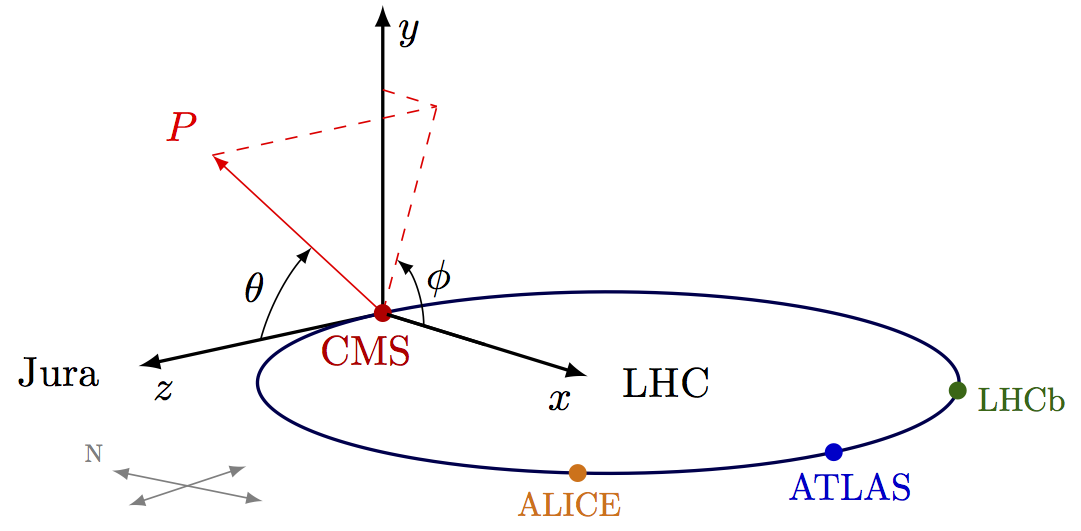
\includegraphics[width=0.8\textwidth]{Images/coordinatechart.png}
	\captionof{figure}{Coordinate system employed by the CMS experiment (retrieved from~\parencite{cmsplots}).}\label{fig_coordinates}
\end{center}

The event rate $R$ for a physical process (e.g., $pp \to X$) is governed by the accelerator's luminosity $\mathcal{L}$ and the process cross section $\sigma$. Luminosity quantifies the performance of a collider to produce interactions, establishing the proportionality,
\begin{equation}
	\frac{d R}{d t} = \mathcal{L} \sigma,
\end{equation}
where $\sigma$ (typically measured in barns, $1\,\text{b} = 10^{-24}\,\text{cm}^2$) encodes the interaction probability. For LHC proton bunches colliding head-on with Gaussian transverse profiles, the instantaneous luminosity is~\parencite{Herr:941318,book:1123430}:
\begin{equation}
	\mathcal{L} = \frac{f N_{b}}{4\pi} \frac{N_{1} N_{2}}{\sigma_{x} \sigma_{y}}\label{eq_lumi}
\end{equation}
Here, $N_{1,2}$ are proton counts per bunch, $f$ is the bunch collision frequency, $N_{b}$ is the number of bunches, and $\sigma_{x,y}$ are transverse beam widths. 

Integrating $\mathcal{L}$ over time yields the total integrated luminosity $L$, linking directly to the observed event count $N$:
\begin{equation}
	L = \int \mathcal{L}\, dt \quad \Rightarrow \quad N = L \sigma.
\end{equation}
%At Run~II luminosities ($\mathcal{L} \approx 1.5 \times 10^{34}\,\text{cm}^{-2}\text{s}^{-1}$), a $1\,\text{pb}$ cross section produces $\sim\!15$ events per second. This framework underpins all LHC physics analyses, from Higgs measurements ($\sigma_{pp\to H} \sim 50\,\text{pb}$ at $13\,\text{TeV}$) to BSM searches for rare processes ($\sigma_{\text{BSM}} \ll 1\,\text{fb}$).
  
The Gaussian beam approximation in~\eqref{eq_lumi} ignores hourglass effects (beam divergence near interaction points) and dynamic $\sigma_{x,y}$ variations during fills. CMS mitigates these via real-time luminosity monitoring using pixel clusters~\parencite{Sirunyan2021}, with systematic uncertainties below $2\%$. High $\mathcal{L}$ also introduces pileup—multiple $pp$ interactions per bunch crossing—which complicates $\eta$/$\phi$ measurements but is corrected using vertex isolation algorithms.


The most important parameters of an accelerator are the following:
\begin{description}

	\item[Centre-of-mass energy]  $(\sqrt{s})$ The energy of the colliding particles in the centre-of-mass (CM) frame. Since the total momentum of the particles in the CM frame is zero, the CM energy is simply the square-root of the total 4-momentum:
	$$
	\begin{gathered}
		\sqrt{s}=\sqrt{P^{\mu} P_{\mu}}, \\
		P^{\mu}=\sum_{i} p_{i}^{\mu}.
	\end{gathered}
	$$
	The energy in the CM frame must be greater than the total mass of the particles being produced. Thus, the CM energy determines which particles can be studied in the accelerator.
\end{description}
\begin{center}
  		% CMS detector - left perspective
		\tdplotsetmaincoords{75}{50} % to reset previous setting
		\begin{tikzpicture}[scale=2.6,tdplot_main_coords,rotate around x=90]
			
			% VARIABLES
			\def\rvec{\L/2/cos(\thetavec)}
			\def\thetavec{18}
			\def\phivec{60}
			\def\L{3.3}    % detector length
			\def\R{0.75}   % detector cylinder radius
			\def\l{4.3}    % beam pipe length
			\def\r{0.04}   % beam pipe radius
			\def\rt{0.042} % beam pipe radius + line thickness
			\def\xmax{1}   % maximum x axis
			\def\ymax{1}   % maximum y axis
			\def\zmin{-\l/2-0.2} % minimum z axis
			\def\zmax{\l/2+0.3}  % maximum z axis
			\def\w{0.3}
			\coordinate (O) at (0,0,0);
			\coordinate (Z) at (0,0,\L/2);
			\tdplotsetcoord{O'}{0.022}{\thetavec}{\phivec} % slightly shifted origin
			\tdplotsetcoord{O''}{0.018}{90}{\phivec} % slightly shifted origin
			\tdplotsetcoord{P}{\rvec}{\thetavec}{\phivec}
			
			% CYLINDER behind
			\def\ang{19} % rotate lines to simulate cylinder
			\fill[top color=red!50!black!4,bottom color=red!60!black!2,rotate around z=\ang]
			(0,\R,\L/2) --++ (0,0,-\L) arc(90:270:\R) --++ (0,0,\L) arc(270:90:\R) -- cycle;
			\fill[detector surface] % transverse plane at z=L/2
			(0,0,\L/2) --++ (0,\R,0) arc(90:270:\R) -- cycle;
			\fill[detector surface] % transverse plane at z=-L/2
			(0,0,-\L/2) --++ (0,\R,0) arc(90:270:\R) -- cycle;
			\tdplotdrawarc[detector]{(0,0,\L/2)}{\R}{0}{360}{}{}
			\tdplotdrawarc[detector,thin]{(0,0,-\L/2)}{\R}{0}{360}{}{}
			%\draw[detector,canvas is yx plane at z=-\L/2] (0,0,0) circle(\R);
			\draw[detector,thin, dashed] % transverse plane at z=0
			(90-\ang:\R) arc (90-\ang:270:\R);
			\draw[detector] (0,0,-\L/2)++(90:\R) --++ (0,0,\L); % top horizontal
			\draw[detector] (0,0,-\L/2)++(-90:\R) --++ (0,0,\L); % bottom horizontal
			
			% BEAM PIPE
			\tdplotdrawarc[beam pipe]{(0,0,\l/2)}{\r}{0}{360}{}{}
			%\tdplotdrawarc[beam pipe]{(0,0,-\l/2)}{\r}{\ang-90}{90}{}{}
			%\draw[beam pipe] % cylindric beam pipe
			%  (0,\r,-\l/2) --++ (0,0,\l) arc(90:-90:\r)
			%  --++ (0,0,-\l) arc(-90:90:\r);
			\draw[beam pipe] % beam pipe, thinner in middle
			(0,\r,-\l/2) -- (0,\r,-0.2*\l) -- (90:0.5*\r)
			-- (0,\r,0.2*\l) -- (0,\r,0.5*\l) arc(90:-90:\r)
			-- (0,-\r,0.2*\l) -- (-90:0.5*\r) --
			(0,-\r,-0.2*\l) -- (0,-\r,-\l/2) arc(-90:90:\r);
			\draw[beam pipe] (0,0,\l/2) circle(\r);
			
			% AXES
			%\draw[thick,->] (0,0,0) -- (0,0,1) node[below right]{$z$}; % short
			\draw[axis,-] (0,0,\zmin) -- (0,0,0); % long
			\fill[CMScol] (O) circle(0.5pt) node[right=1,below=1] {IP};
			\draw[axis] (0,0,0.020) -- (0,0,\zmax) node[right=3,above=0.1]{$z$}; % long
			\draw[axis] (0,0.019,0) -- (0,\ymax,0) node[below left]{$y$};
			\draw[axis] (0.022,0,0) -- (\xmax,0,0) node[below=1,right=-2]{$x$};
			
			% LABELS
			\node[mydarkred,above] at (0,\ymax,0) {$\eta=0$};
			\node[mydarkred,above=0.6, left] at (0,\R,0.3*\L) {$\eta>0$};
			\node[mydarkred,above=0.7, right] at (0,\R,-0.2*\L) {$\eta<0$};
			\node[mydarkred,below=1,left] at (0,0,\zmax) {$\eta=\infty$};
			\node[mydarkred,above=1,right] at (0,0,\zmin) {$\eta=-\infty$};
			
			% VECTORS
			%\fill[radius=0.4,red] (P) circle;
			\draw[dashed,myred] (P)  -- (Pxy);
			\draw[dashed,myred] (Py) -- (Pxy);
			\draw[dashed,myred] (P) -- (Pz);
			
			
			\draw[->,miverde,line cap=round,draw opacity=0.9] (O') -- (P) node[anchor=-30] {\contour{white}{$\va*{p}$}};
			\draw[->,miverde,line cap=round] (O') -- (P) node[anchor=-30] {$\va*{p}$};
			
			\draw[->,azulF,line cap=round,draw opacity=0.9] (O') -- (Pxy) node[right, anchor=-100] {\contour{white}{$\va*{p}_T$}};
			% \draw[->,azulF,line cap=round] (O') -- (Pxy) node[right , anchor=-100] {$\va*{p}_T$};
			
			
			% CYLINDER front
			\draw[beam pipe,fill=none] (0,\r,-\l/2) arc(90:-90:\r);
			\fill[detector surface] % transverse plane at z=L/2
			(0,\rt,\L/2) --++ (0,\R-\rt,0) arc(90:-90:\R) --++ (0,\R-\rt,0) arc(-90:90:\rt);
			\fill[detector surface] % transverse plane at z=-L/2
			(0,\rt,-\L/2) --++ (0,\R-\rt,0) arc(90:-90:\R) --++ (0,\R-\rt,0) arc(-90:90:\rt);
			\tdplotdrawarc[detector]{(0,0,\L/2)}{\R}{-90}{90}{}{} % transverse plane at z=L/2
			\tdplotdrawarc[detector]{(0,0,-\L/2)}{\R}{-90}{90}{}{} % transverse plane at z=-L/2
			\draw[beam pipe,fill=none] (0,\r,\l/2) arc(90:-90:\r);
			\draw[detector,very thin, dashed] % transverse plane at z=0
			(90-\ang:\R) arc (90-\ang:-90:\R);
			
			% ANGLES
			\tdplotdrawarc[thick,red!57!black!3] % contour
			{(O)}{0.2}{4}{0.7*\phivec}{}{}

			% white to contour
			\tdplotdrawarc[draw=azulF, line width=0.6pt, draw opacity=0.9]{(O)}{0.2}{0}{\phivec}{above=2,right=0.75,anchor=-30,text=black}{\contour{white}{$\phi$}}
			\tdplotdrawarc[->, azulF]{(O)}{0.2}{0}{\phivec}{above=2,right=0.75,anchor=-30}{$\phi$}


			\tdplotdrawarc[->,rotate around z=\phivec-90,rotate around y=-90]
			{(O)}{0.88}{0}{\thetavec}{anchor=mid east}{$\theta$}
			\tdplotdrawarc[thick,red!58!black!4,rotate around z=\phivec-90,rotate around y=-90] % contour
			{(O)}{0.3}{88}{0.5*(90+\thetavec)}{}{}
			\tdplotdrawarc[-{>[flex'=1]},rotate around z=\phivec-90,rotate around y=-90,line cap=round]
			{(O)}{0.3}{90}{\thetavec}{above=4.5,right=0.5,anchor=mid east}{$\eta$}
			\draw[mydarkred] (0,0,\L/2) --++ (\R,0,0);
			\tdplotdrawarc[thick,red!60!black!6] % contour
			{(Z)}{0.2}{4}{0.7*\phivec}{}{}
			\tdplotdrawarc[draw=none,opacity=0.8]{(Z)}{0.2}{0}{\phivec}{above=2,right=0.7,anchor=-30}{\contour{red!60!black!6}{$\phi$}}
			\tdplotdrawarc[->]{(Z)}{0.2}{0}{\phivec}{above=2,right=0.7,anchor=-30}{$\phi$}
			
			% COMPASS - CMS-ATLAS axis has a ~12° declination (http://googlecompass.com)
			\begin{scope}[shift={(1.1*\R,-\R,0.2*\L)},rotate around y=12]
				\draw[<->,black!50] (-\w,0,0) -- (\w,0,0);
				\draw[<->,black!50] (0,0,-\w) -- (0,0,\w);
				\node[left,black!50,scale=0.6] at (-\w,0,0) {N};
				\node[below=3,left=-2,green!20!black!50,scale=0.6] at (0,0,\w) {Jura};
				%\node[below=1,right,black!50,scale=0.6,align=center] at (\w,0,0) {center of\\the LHC};
				%\node[below=1,right,blue!30!black!50,scale=0.6] at (\w,0,0) {ATLAS};
			\end{scope}
			\draw[->,thick,orange!30!black] (1.4*\w,-\R,-0.1*\L) --++ (2*\w,0,0)
			node[right,scale=0.8,align=center] {center of\\[-1pt]the LHC};
			
		\end{tikzpicture}
  \captionof{figure}{Detailed reparametrization of the coordinate system employed by the CMS experiment (retrieved from~\parencite{cmsplots})}\label{fig_cms_coor}
\end{center}
The following variables are related to the particles being produced rather than the accelerator.
\begin{description}
	\item[Decay width] ( $\Gamma)$ The decay rate is the probability that a given particle will decay per unit time. Since a particle can have multiple decay modes, the total decay rate is the sum of the decay rates for each mode~\parencite{book:1123430}. The relative frequency of a decay mode is the branching ratio, given by
	$$
	\mathrm{BR}(j)=\frac{\Gamma(j)}{\Gamma} .
	$$
	\item[Cross-section] $(\sigma)$ The cross-section is a measure of the probability that an interaction will occur from a collision. It is a quantum-mechanical analogue of the "effective size" of the particles involved in an interaction.

	\item[Pseudo-rapidity] $(\eta)$ Instead of using the polar angle, CMS measurements involve the pseudo-rapidity, defined by
	$$
	\eta=-\ln \left(\tan \frac{\theta}{2}\right)
	$$
	The main advantage of using the pseudo-rapidity is that distributions over it tend to be closer to a uniform distribution than those over the polar angle, see Fig.~\ref{fig_cms_coor}. Furthermore, the difference in pseudo-rapidity is invariant under Lorentz boosts along the beam direction~\parencite{book:1123430}.
	\item[Transverse Momentum] ($p_T$) Refers to the component of momentum which is perpendicular to the beam line. It is usually preferred over full momentum because momentum along the beamline may just be left over from the beam particles, while the transverse momentum is always associated with whatever physics happened at the vertex, see Fig.~\ref{fig_cms_coor}.
	\item[Missing transverse energy and momentum] $\left(E_{T}^{\text {miss }} \& p_{T}^{\text {miss }}\right)$ Missing energy and momentum refers to the energy and momentum that is not detected but is expected to be there as a consequence of energy conservation and momentum conservation. This momentum is often carried by particles that do not interact electromagnetically or strongly and are therefore difficult to detect~\parencite{book:1123430}. Missing energy and momentum provides an indirect measurement of undetectable particles in hadron colliders such as neutrinos. Missing momentum reconstructions focus on the transverse direction, where total momentum is expected to be zero.
\end{description}


\section{Detectors and Subsystems}

A typical collider experiment comprises several main detector subsystems that are used jointly to detect and measure the properties of particles produced in the collision. A \textit{schematic representation} of such a generic multipurpose detector is shown in Fig.~\ref{fig_detector}. The detector is typically composed of several concentric layers, each designed to measure different properties of the particles produced in the collisions. 

\begin{center}
	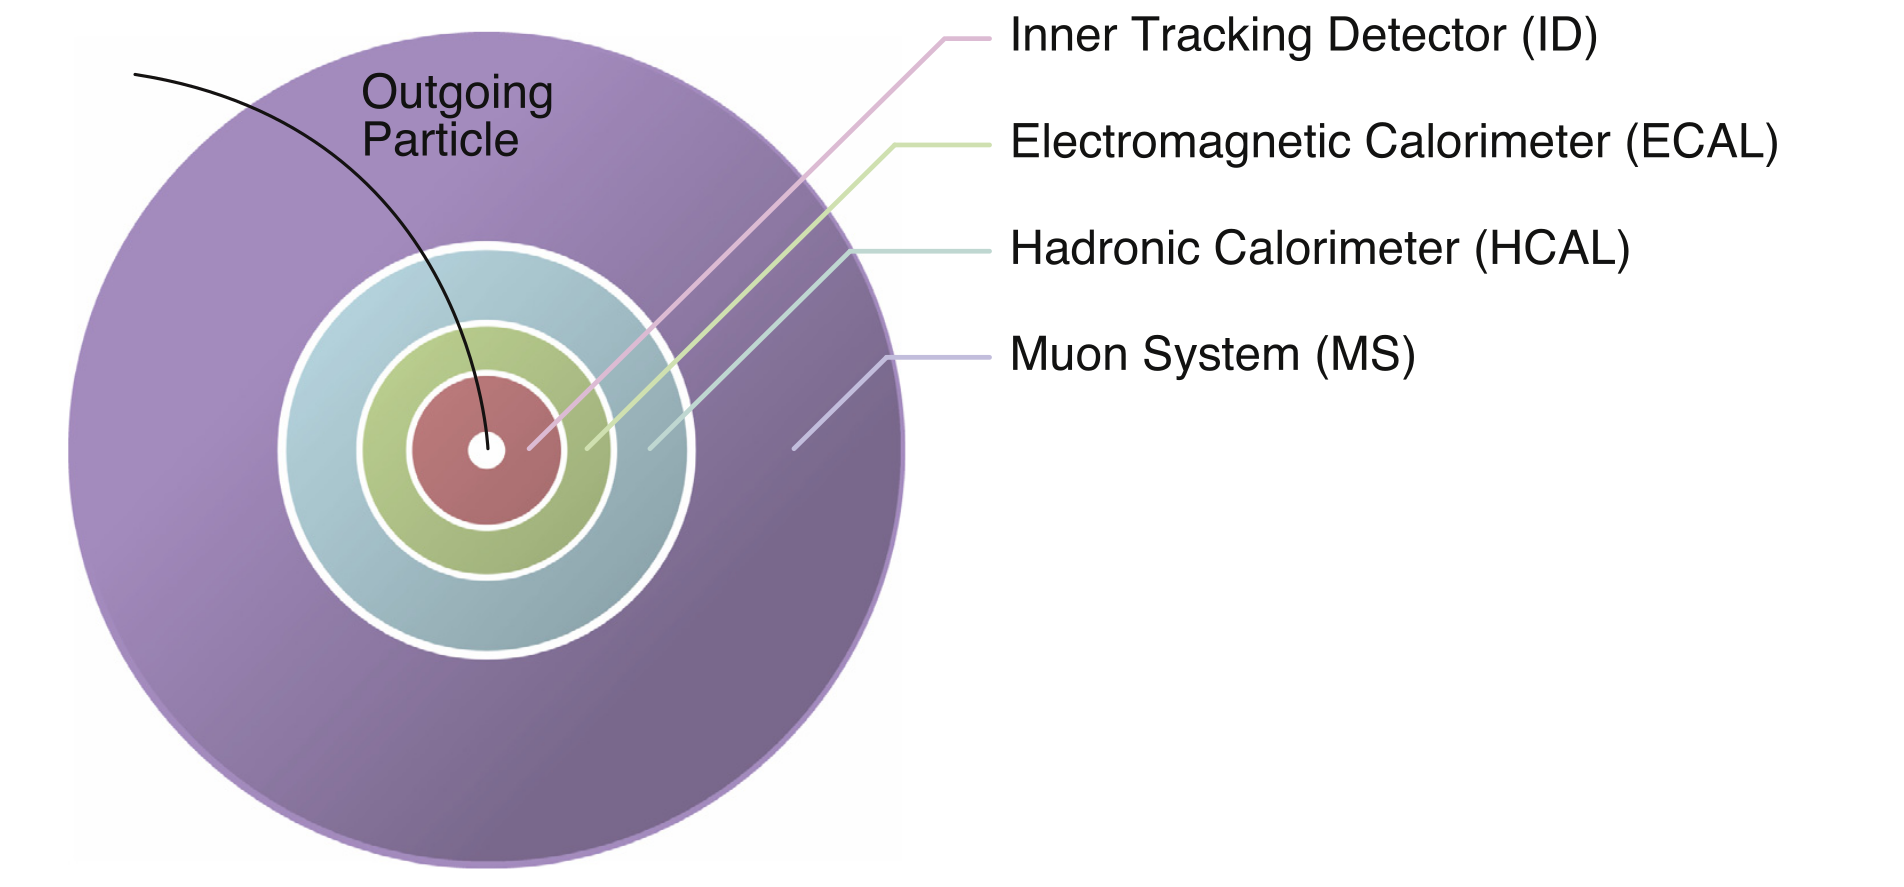
\includegraphics[width=0.98\textwidth]{Images/detector.png}
	\captionof{figure}{Schematic representation of a generic multipurpose detector (retrieved from~\parencite{cmsplots})}\label{fig_detector}
\end{center}

The innermost subsystem, called the inner detector (ID), is designed to detect electrically charged particles that are long-lived enough to traverse the ID. The most common such particles from the SM are two charged leptons (the electron $e$ and the muon $\mu$ ) and three hadrons (the pion $\pi$, kaon $K$, and proton $p$ ). Regions of ionization produced by such a particle in solid-state or gaseous detector sensors are detected as spatial hits that are fit into a trajectory, referred to as a \textbf{track}. The direction and curvature of the track in a magnetic field yield the particle's momentum vector and electric charge. In some detectors, the ID is enclosed in a Cherenkov-light detector used to measure the velocity of the tracked particles. Combined with the momentum measurement in the ID, this yields the particle mass with sufficient resolution to differentiate between pions, kaons, and protons in a relevant momentum range.

After passing through the tracker, particles produced in the collisions typically enter an electromagnetic calorimeter (ECAL), designed to measure the energies of photons, electrons and positrons. The energy measurement exploits the properties of electromagnetic shower production via photon radiation and $e^{+} e^{-}$ pair production, resulting from the interaction of energetic particles with the ECAL material.

Hadrons deposit energy via hadronic interactions with the detector material. Since this process involves large fluctuations and a variety of energy-deposition mechanisms, precise hadron-energy measurement is achievable only at high-energy colliders, where fluctuations are effectively averaged out. In particular, high-energy quarks and gluons hadronize into a collimated spray of hadrons known as a \textbf{jet}. Containing the jet requires use of a deep hadronic calorimeter (HCAL) beyond the ECAL. While a jet can be identified solely in the calorimeters, its energy is nowadays measured from a combination of the momenta of tracks in the ID and the signals integrated in the ECAL and HCAL. 

The signals from the calorimeters, know as \textbf{towers}, are grouped into jets using a jet clustering algorithm. If and hadronic particle is neutral, it will not leave a track in the ID, but it will still deposit energy in the towers. So, the towers are used to measure the energy of neutral particles, such as photons and neutral hadrons, while the ID tracks are used to measure the energy of charged particles. This approach is known as particle flow (PF) reconstruction and provides a more accurate measurement of the energy of jets. 

Muons do not undergo hadronic interactions, and are heavy enough that they lose energy due to ionization at a low rate. Therefore, they lose only a few GeV while traversing a typical LHC-detector calorimeter. Using this property to identify them, a muon system (MS) is built outside the calorimeter. In high-energy collider detectors, the MS is usually immersed in a magnetic field in order to measure the momenta of muons. Tracks reconstructed in the MS are often combined with tracks in the ID to obtain a high-quality momentum measurement.

When studying final states that include long-lived, weakly interacting particles, such as neutrinos in the SM or dark matter candidates in BSM models, an important reconstructed quantity is missing momentum.  Using three-momentum conservation and the approximate hermeticity of the detector, it is possible to measure the momentum imbalance in the event and to infer the combined momentum of the invisible set of particles. Since the interacting partons in proton collisions generally carry different fractions of the momenta of the incoming hadrons and many of the particles produced fall outside of the acceptance of the sensitive detector, the summed momenta of measured final-state particles along the beam axis $z$ are not expected to cancel. Therefore, experiments at the LHC measure the missing transverse momentum, denoted $E_{\mathrm{T}}^{\text {miss }}$ known as Missing Energy Transverse (\textbf{MET}), where momentum balance is assumed only in the $x-y$ plane transverse to the beam direction.

Collider detectors are mostly designed and constructed for optimal detection of SM particles produced in the collision. However, they can also be used to search for new physics (NP) beyond the SM. In this case, the detector is used to search for signatures of NP, such as new particles or interactions that are not predicted by the SM. The detector subsystems are designed to be sensitive to a wide range of particles and interactions, allowing for the detection of a variety of NP signatures.

\subsection{Jets Reconstruction}

At the LHC, jets are reconstructed as proxies for the quarks and gluons produced in the hard scattering process. Due to color confinement, these partons cannot be observed directly, and instead hadronize into collimated sprays of particles. These sprays are clustered into jets using algorithms that group together the signals of their constituents in the detector.

The most widely used algorithm in ATLAS and CMS is the anti-$k_T$ clustering algorithm~\parencite{Cacciari:2008gp}, implemented in the \texttt{FastJet} package~\parencite{Cacciari:2011ma}. This algorithm groups particle candidates or calorimeter deposits into jets based on their proximity in the rapidity-azimuth $(y,\phi)$ plane, with a distance parameter $R$ typically set to values like 0.4 or 0.6. The resulting jets have a regular conical shape and are relatively insensitive to soft radiation and pileup.

Modern jet reconstruction exploits particle-flow (PF) algorithms, which combine information from all detector subsystems to reconstruct individual particles (charged hadrons, neutral hadrons, photons, electrons, and muons). The momenta of PF candidates are then used as input for jet clustering. This approach improves the resolution of jet energy and direction, especially at low transverse momentum.

After clustering, several levels of jet energy corrections (JEC) are applied to account for detector response, pileup, and underlying event contributions. These corrections are derived from simulation and in-situ calibrations using well-known processes like dijet balance or photon+jet events.

\subsection{$\tau$ Tagging at Multipurpose Detectors}

The tau lepton, being the heaviest charged lepton in the SM, decays promptly into either a lighter lepton (electron or muon) and neutrinos, or into hadrons and a tau neutrino. About 65\% of taus decay hadronically, producing narrow jets with a characteristic signature.

Hadronic tau decays ($\tau_{\text{had}}$) typically produce one or three charged hadrons (predominantly pions) and up to two neutral pions, which decay into photons. These decay products result in a collimated energy deposit in the calorimeters and a small number of associated tracks. Tau jets are thus narrower than QCD jets and have lower track multiplicity.

Tau identification algorithms at the LHC exploit these features by using multivariate techniques that combine:
\begin{itemize}
    \item the number of charged and neutral constituents,
    \item the collimation of energy deposits,
    \item isolation criteria based on the surrounding activity,
    \item the invariant mass of the visible decay products,
    \item and lifetime-related variables (e.g., impact parameter significance).
\end{itemize}

In CMS, the Hadron Plus Strips (HPS) algorithm reconstructs the decay mode and applies discriminants to distinguish taus from jets, electrons, and muons~\parencite{CMS:2022ydz}. ATLAS uses similar methods, with Boosted Decision Trees (BDTs) trained to separate taus from background~\parencite{ATLAS:2022fgo}.

Typical tau tagging efficiencies are around 60\% for hadronic taus, with misidentification rates of about 1\% for quark/gluon jets, depending on the working point.

\subsection{B Tagging at Multipurpose Detectors}

Jets originating from bottom quarks ($b$-jets) exhibit distinct features due to the relatively long lifetime ($\sim 1.5$ ps) and large mass ($\sim 4.2$ GeV) of the $b$ hadrons. These hadrons travel a few millimeters before decaying, often producing secondary vertices displaced from the primary interaction point.

$b$-tagging algorithms exploit this property by reconstructing tracks with large impact parameters and identifying displaced secondary vertices. Some algorithms also make use of the presence of soft leptons inside the jet from semileptonic $b$ decays.

Classical algorithms include:
\begin{itemize}
    \item \textbf{Track Counting:} based on the number of tracks with high impact parameter.
    \item \textbf{Jet Probability:} uses the probability that the jet’s tracks originate from the primary vertex.
    \item \textbf{Secondary Vertex:} reconstructs displaced vertices within the jet.
\end{itemize}

Modern approaches rely on machine learning techniques to combine multiple observables. CMS uses DeepCSV and DeepJet algorithms~\parencite{CMS:2017wtu}, based on deep neural networks. ATLAS employs algorithms like MV2 and DL1~\parencite{ATLAS:2019bwq}. These classifiers achieve improved performance in distinguishing $b$-jets from $c$-jets and light-flavor jets.

Typical $b$-tagging efficiencies range from 60\% to 80\%, depending on the working point, with light-jet misidentification rates of 1\% or lower. Calibrations are performed using data-driven methods in control samples enriched in $t\bar{t}$ or multijet events.

\subsection{The CMS Detector}
Particularly the CMS multi-purpose detector has a length of $21.6$ meters, with a diameter of $14.6$ meters and weights 12500 tonnes. The detector is composed of a set of different sub-detectors as seen in figure \ref{fig_cms}. The CMS detector has a cylindrical shape and it is divided into two main sections: barrel and endcaps. 

\begin{center}
	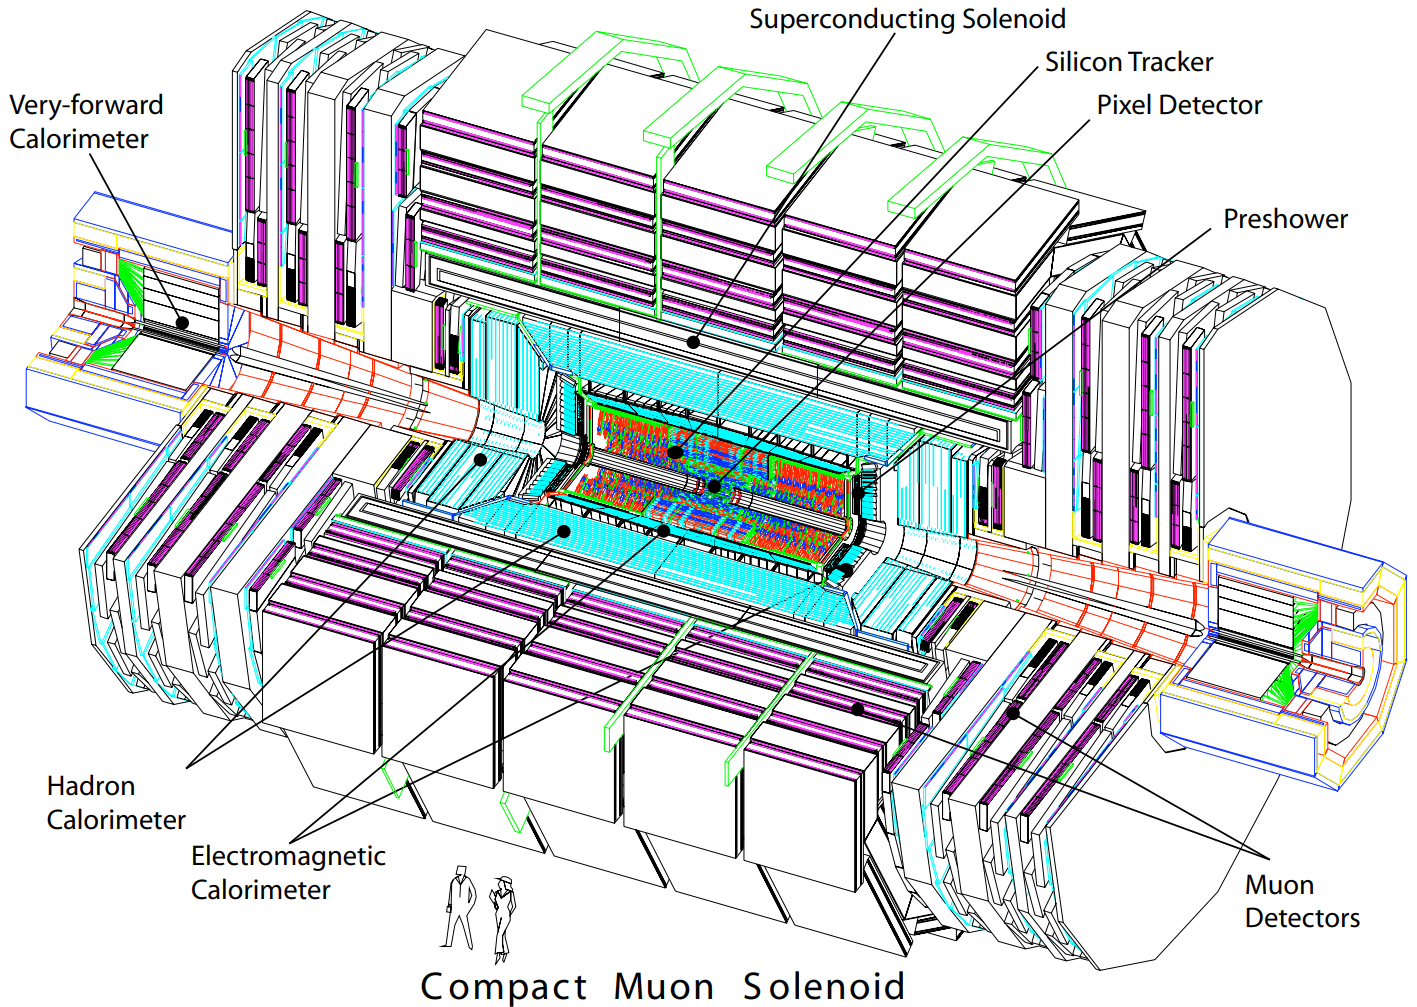
\includegraphics[width=0.98\textwidth]{Images/CMS.png}
	\captionof{figure}{Diagram of the CMS detector showing inner components (retrieved from~\parencite{Collaboration_2008})}\label{fig_cms}
\end{center}

The different sub-detectors are located concentrically in layers~\parencite{Collaboration_2008}. The inner most layer has a pixel detector made out of silicon, used for the reconstruction of primary and secondary vertices from electrically charged particles that decay promptly within this sub-detector volume. The pixel detector is followed by a sub-detector made of silicon strips, known as the tracker detector, used for the reconstruction of trajectories of electrically charged particles. Following the tracker detector, are found the electromagnetic (ECAL) and hadron (HCAL) calorimeters, used to measure both energy and direction of the particles undergoing electromagnetic and strong interactions, respectively. The ECAL detector is a modular device composed of lead-tugsten crystals, highly efficient to produce electromagnetic showers after interacting with charged particles. The emerging photons from the showers are measured using photo-diodes, that collect the light produced from the signal and convert it into an electric signal. This signal is then used by software tools to detect the energy and direction of the corresponding particles~\parencite{Collaboration_2008}. The ECAL is made of non magnetic materials such as copper and steel, which are characterized by heavy nuclei favoring strong interactions. Following a similar functioning as ECAL, hadronic particles enter the calorimeter, interact with the non-magnetic layers producing hadronic showers. These showers are then detected by plastic scintillators and their signals are transformed into electric pulses. These signals are then analyzed to estimate the energy and direction of the original particles~\parencite{Collaboration_2008}.

The next layer of the detector consists of a superconducting solenoid, which surrounds the previous sub-detectors. This solenoid is made of a niobum-titanium alloy that is refrigerated to $2 \mathrm{~K}$ by using liquid helium, producing a uniform magnetic field of $3.8 \mathrm{~T}$ inside the barrel~\parencite{Collaboration_2008}. This magnetic field is used to measure the momentum of electrically charged particles as it induces curvatures in their trajectories.

Finally, the last set sub-detectors conform the muon detector system. This system is made of three different detector technologies, that allow to reconstruct the trajectory of the muons with a fast trigger response, and are alternated with iron returning yokes of steel to enclose the magnetic field produced by the solenoid. The trigger is a date-filtering system composed of hardware and software algorithms, designed to collect interesting events from the proton-proton collisions. The muon detectors have a total of 1400 chambers distributed in 250 drift tubes, 540 cathode strip chambers that track the position of a muon and provide a trigger, as well as 610 resistive plate chambers that give a redundant trigger, which quickly decide over the event storage~\parencite{Collaboration_2008}.

% To do: ADD related with aceptance and efficiency in the barrel and endcaps.

Due to its cylindrical geometry, the CMS detector is divided into a central barrel region and two forward endcaps, which define the detector acceptance in terms of the pseudorapidity. The barrel region provides coverage for $|\eta| \lesssim 1.5$, while the endcap regions extend the acceptance up to $1.5\lesssim|\eta| \lesssim 2.5$ for most subsystems~\parencite{Collaboration_2008}. 

This geometrical segmentation impacts the overall detection efficiency. For example, the pixel and silicon strip trackers are more efficient in the barrel, where multiple tracking layers are crossed perpendicularly by particles. In the endcaps, particles cross detector layers at shallow angles, leading to reduced hit multiplicity and, consequently, lower tracking efficiency and resolution. Similar considerations apply to the ECAL and HCAL subsystems, where the granularity and material budget have been optimized to compensate for the non-uniform geometry, maintaining energy resolution across $\eta$.

Muon identification and momentum reconstruction also exhibit regional differences. The drift tubes (DTs), which offer high spatial resolution, are only installed in the barrel, while cathode strip chambers (CSCs) and resistive plate chambers (RPCs) cover the endcap regions. The combination of technologies ensures redundancy and robust triggering throughout the full detector acceptance. However, due to the higher background levels and increased radiation in the endcaps, the performance of muon reconstruction tends to be better in the barrel. For muons (electrons), the assumed identification efficiency is 95\% (85\%), with a 0.3\% (0.6\%) mis-identification rate~\parencite{CMS-PAS-FTR-13-014,CMS_MUON_17001,CMS_EGM_17001}.

Following reference~\parencite{CMS_BTV2016}, we use a flat identification efficiency for $\bq$ jets of 70\% across the entire $\pt$ spectrum with misidentification rate of 1\%. These values correspond with the  ``medium working point'' of the CMS algorithm to identify $\bq$ jets, known as DeepCSV. We also explored the ``Loose'' (``Tight'') working point using an efficiency of 85\% (45\%) and mis-identification rate of 10\% (0.1\%). 

For the performance of $\tau_{\textrm{h}}$ identification in DELPHES, we consider the latest technique described in~\parencite{CMS_DeepTau}, which is based on a deep neural network (i.e. DeepTau) that combines variables related to isolation and $\tau$-lepton lifetime as input to identify different $\tau_{\textrm{h}}$ decay modes. Following~\parencite{CMS_DeepTau}, we consider three possible DeepTau ``working points'': (i) the ``Medium'' working point of the algorithm, which gives a 70\% $\tau_{\textrm{h}}$-tagging efficiency and 0.5\% light-quark and gluon jet mis-identification rate; (ii) the ``Tight'' working point, which gives a 60\% $\tau_{\textrm{h}}$-tagging efficiency and 0.2\% light-quark and gluon jet mis-identification rate; and (iii) the ``VTight'' working point, which gives a 50\% $\tau_{\textrm{h}}$-tagging efficiency and 0.1\% light-quark and gluon jet mis-identification rate. Similar to the choice of $\textrm{b}$-tagging working point, the choice of $\tau_{\textrm{h}}$-tagging working point is determined through an optimization process which maximizes discovery reach. The ``Medium'' working point was ultimately shown to provide the best sensitivity and therefore chosen for this study. 

\section{Phenomenological Pipeline}
For the study of hypothetical signals for these new models and their feasibility of observation in experiments such as the LHC, one of the most widely used methods is the generation of events in colliders via Monte Carlo computational simulations. Monte Carlo simulation (MC) are used to predict what we expect to see under certain conditions:

\begin{itemize}
	\item To perform calculations in an automated way, such as, cross sections and disintegration widths.
	\item To perform studies before having the data.
	\item To compute event selection efficiency / acceptance.
	\item To predict the amount of background events.
	\item To distinguish different signals.
\end{itemize}

Today, there is a wide set of independent and modular tools that simulate the different experimental stages and that allow us to calibrate and contrast with relative ease the simulated results with the experimental ones. For pp collision simulations, the use of MadGraph5\_aMC@NLO (MadGraph)~\parencite{Alwall_2014} framework is widespread.

MadGraph is a modular working environment, that is, simulation occurs in several stages. First MadGraph receives the information with the Feynman rules of a specific model in a format known as Universal Feynman Output (UFO) (which is generated from the Lagrangian in Wolfram Mathematica with the use of the FeynRules library~\parencite{ALLOUL20142250}), along with a parameter card with the numerical values of the free parameters of the Lagrangian. 

With this information MadGraph creates a directory with all the diagrams and amplitudes of a given process (Output folder). Then a subroutine known as MadEvent is run that generates \textit{hard scatter events} and creates a known output in LHE format with the information of the four vectors of each particle of the final state. Normally, to optimize the generation with MadEvent, we can modify the so-called run\_card such that the output partons are in a state to be subsequently reconstructed in the detector. If we generate events whose partons will be ignored by the detector we are wasting computational power. 

Then, we can take the information from the LHE output to simulate the parton shower and the hadronization of the final state. This process is typically done with Pythia8 (Pythia)~\parencite{2203.11601}, which is possibly the most complete MC generator to simulate the parton shower and the hadronization. Here, we have the advantage that it is implemented to run automatically within MadGraph. 

Pythia output is in HepMC2 format. With this information we run a software, DELPHES~\parencite{de_Favereau_2014}, that performs a fast simulation of the detector response to interactions with particles. The output of DELPHES is in ROOT format ready for a data analysis in ROOT framework. From this point, the analysis is similar to that done in each of the experiments using the data delivered by the detector, although with an extra processing layer such as tagging processes of some particle candidates, such as light jets, b-jets, and hadronic taus.

\section{Measurement of the Power of an Analysis}
\label{sec:power_analysis}

The statistical power of an analysis quantifies its sensitivity to discriminate between signal and background processes. For binned data following Poisson statistics, we define the power $\kappa$ as:

\begin{equation}
\kappa = \frac{\sum_i s_i w_i}{\sqrt{\sum_i \left(s_i + b_i\right) w_i^2}},
\label{eq:kappa_definition}
\end{equation}

where:
\begin{itemize}
    \item $s_i$ and $b_i$ are the expected signal and background events in bin $i$
    \item $w_i$ is the optimal weight for bin $i$, given by:
    \begin{equation}
        w_i = \ln\left(1 + \frac{s_i}{b_i}\right)
        \label{eq:optimal_weights}
    \end{equation}
\end{itemize}

\subsection*{Special Case: Single Bin Analysis}
For a single bin with strong signal ($s \gg b$), Eq.~\ref{eq:kappa_definition} reduces to the Poisson significance:

\begin{equation}
\kappa \approx \frac{s}{\sqrt{s + b}},
\label{eq:single_bin_kappa}
\end{equation}

\subsection*{Incorporating Systematic Uncertainties}
The power calculation can be extended to include systematic uncertainties by modifying the denominator:

\begin{equation}
\kappa_{\text{sys}} = \frac{\sum_i s_i w_i}{\sqrt{\sum_i \left[(s_i + b_i) + \sigma^2_{\text{sys,signal},i} + \sigma^2_{\text{sys,bkg},i}\right] w_i^2}},
\label{eq:kappa_with_systematics}
\end{equation}

where $\sigma_{\text{sys}}$ terms represent the systematic uncertainties on signal and background predictions.
\chapter{LHC Observables, Experimental Searches, and Analysis Strategies}
\chapter{ Probing Light Scalars and Vector-like Quarks at the High-Luminosity LHC}

% \section{Introduction}
% \label{introduction}


The Standard Model (SM) of particle physics, despite its successful account of numerous experimental findings involving strong, electromagnetic, and weak interactions, confirmed by CERN's Large Hadron Collider (LHC) is regarded as a lower-energy manifestation of a more comprehensive theory. This perspective arises from unresolved questions regarding the origins of dark matter, electroweak symmetry breaking scales, lepton flavor universality, the anomalous muon magnetic moment~\parencite{PhysRevD.73.072003, g2cit,Davier2017,Davier2020,PhysRevLett.121.022003,PhysRevD.97.114025,PhysRevLett.124.132002,PhysRevD.100.076004}, discrepancies in the $R_{(D)}$ and $R_{(D^{*})}$ ratios from $\mathrm{b}$-meson decays~\parencite{ BaBar:2012obs,BaBar:2013mob, Huschle:2015rga,LHCb:2015gmp,Aaij:2015yra,Sato:2016svk, Hirose:2016wfn, Aaij:2017uff, Hirose:2017dxl,LHCb:2017rln,Abdesselam:2019dgh,Belle:2019rba,LHCb:2023zxo}, as well as theoretical conundrums about whether gravity should be quantized, how gauge interactions can be unified, and the fine-tuning problem associated with the Higgs boson mass. Furthermore, the SM offers no explanation for fermion family replication nor for the lack of CP violation in the strong sector. These theoretical gaps, coupled with the experimental observation of phenomena such as neutrino masses, dark matter, and the baryon asymmetry in the universe, which cannot be explained by the SM, reinforce the expectation for physics beyond the SM (BSM).

As a result, several theoretical models have been put forth to address the limitations of the SM over the past decade. Despite differing theoretical motivations and resulting implications, a common thread among these ideas is the introduction of new particles, that, depending on the model, might be probed via proton-proton $(\mathrm{pp})$ collisions at the  LHC. A myriad of ideas have been suggested to investigate BSM physics, driving a substantial amount of exploration at the LHC. Said research has significantly limited the scope of theories and established exclusion bounds, extending to multi-\textrm{TeV} ranges for the masses of newly predicted particles within certain models~\parencite{ParticleDataGroup:2024cfk, CMS:2018iye, CMS:2016ucr, CMS:2016xbv, CMS:2016fxb, CMS:2017xcw, CMS:2015jsu}. Possible reasons for the absence of evidence could be attributed to new particle masses being at the scale where they are too large to be produced at the LHC energies and likely with exceptionally low production rates. In the scenario where the masses of the new particles might be probed at the LHC, a vast amount of data might be needed, together with advanced analysis techniques, to enhance the probability of detection. Alternatively, it is conceivable that new physics diverges from the conventional assumptions made in many BSM theories and the associated explorations. As a result, these new physics phenomena could remain hidden in processes that have not yet been thoroughly examined.


Minimal extensions to the SM, considering new $U(1)_{\chi}$ symmetry groups, are among the most studied BSM scenarios. For example, the  $U(1)_{T^3_R}$ symmetry, where families of right-handed fermions of the SM and possible extensions, such as right-handed neutrinos, are charged, was originally studied in the context of left-right symmetry models~\parencite{PatiSalam1974, MohapatraPati1975, SenjanovicMohapatra1975}. In these studies, $U(1)_{T^3_R}$ is identified as the subgroup of $SU(2)_R$ defined by its diagonal (electric-charge neutral) generator, $T^3_R$. In addition, it is often suggested that  $U(1)_{T^3_R}$ is a subspecies of a $U(1)_{B-L}$ symmetry since the breaking of the $U(1)_{B-L} \times U(1)_{T^3_R}$ leads to the $ U(1)_Y$ symmetry. This naturally motivates the presence of a massive and electrically neutral $\textrm{Z}'$ gauge boson~\parencite{DiLuzio2018, Baker2019, Michaels:2020fzj, Dev:2021otb, Florez2023}. However, in the breaking of  $U(1)_{B-L} \times U(1)_{T^3_R} \rightarrow U(1)_Y$, it follows that the Higgs doublet $\mathrm{H}$, since it is a singlet of $U(1)_{B-L}$,  acquires its hypercharge by inheritance from a charge under $U(1)_{T^3_R}$. Consequently, the vacuum expectation value (VEV) of $\mathrm{H}$  couples both symmetry-breaking scales for $U(1)_Y$ and $U(1)_{T^3_R}$. Alternatively, these symmetry-breaking scales can be decoupled by adding an additional $U(1)_G$ group where fermions of the SM are singlets and $\mathrm{H}$ is not. Therefore, the hypercharge comes from $U(1)_G$ for the $\mathrm{H}$ and from $U(1)_{T^3_R}$ for fermions, \textit{i.e.} $Y=Q_{T^3_R}+\frac{1}{2}Q_{B-L} + Q_G$~\parencite{Dutta:2022qvn}. Moreover, one can ask for scenarios where the hypercharge is not related to the $U(1)_{T^{3}_{R}}$ charge. 

Recently, theoretical and phenomenological efforts have emerged around scenarios where the low-energy gauge symmetry of the SM is extended by appending the Abelian gauge group $U(1)_{T^{3}_{R}}$, whose spontaneous symmetry-breaking is not linked to the electroweak one~\parencite{Dutta2019, Dutta2020, Dutta2020b,Dutta2022, PhysRevD.107.095019, Dutta2023}. In these scenarios, the gauge boson of $U(1)_{T^3_R}$ is associated with a massive dark photon $A'$ whose longitudinal mode arises from a Higgs-like mechanism involving a complex scalar field, $\phi$. This field is a singlet under the SM group, with its CP-odd component associated with the $A'$ mass and the CP-even giving rise to a dark Higgs, $\phi'$. To cancel gauge anomalies, a right-handed $\nu_R$ neutrino must be included for each generation of the SM that couples to $U(1)_{T^3_R}$. Furthermore, to correctly explain the origin of fermion masses in a UV-complete theory, a set of new vector-like quarks $(\chi_\mathrm{u}, \chi_d,\chi_\ell, \chi_\nu)$ must be included. These new particles are singlets under $U(1)_{T^3_R}$ and charged like SM right-handed fermions, as in the universal see-saw mechanism~\parencite{Berezhiani, Chang1987, Davidson1987, Rajpoot1987, Babu1989, Babu1990}.

In this phenomenology study, we devise a LHC search strategy for the light \textrm{GeV}-scale scalar boson $\phi'$ produced in association with a heavy \textrm{TeV}-scale $\chi_\mathrm{u}$, the partner particle of the top quark, through a previously unexplored production and final state channel. Particularly, we explore the production of $\mathrm{pp}\to \mathrm{t}\chi_\mathrm{u} \phi'$, in contrast to $\mathrm{pp}\to \mathrm{T}\mathrm{T}\to \mathrm{t}\phi'\mathrm{t}\phi'$ with hadronic~\parencite{Bhardwaj_2022, Bhardwaj_2022_2, Bardhan_2023} di-photonic $\phi'$~\parencite{Banerjee_2016, Alves_2024} decays. Due to the non-trivial $\chi - \mathrm{t} -\phi'$ coupling, processes where the final state includes $ \mathrm{t}\chi_\mathrm{u} \phi'$ are allowed in \textrm{pp} colliders through the ${\chi_\mathrm{u}}{- \mathrm{t}}$ fusion, see Figure~\ref{fig:qqfusion}. Since the $\chi_\mathrm{u}$ couples to SM quarks and gluons, it can be produced in large quantities. Furthermore, its energetic decay products can be detected alongside the $\phi'$ mediator particle that has significant transverse momentum. Therefore, if the $\phi'$ decays into SM particles that are observable in the detector's central region, this strategy can be very effective at reducing the SM background, and thus improve the long-term LHC discovery reach for heavy top partners and~\textrm{GeV}-scale mediators, which are typically hard to detect using conventional methods at hadron colliders. Moreover, since it is possible to have $\chi_\mathrm{u} \to \mathrm{t}\,\phi'$ decays (and $\bar{\chi_\mathrm{u}} \to \bar{\mathrm{t}}\,\phi'$), the same $\mathrm{pp}\to \mathrm{t}\chi_\mathrm{u} \phi'$ state may arise from $\chi_\mathrm{u}\bar\chi_\mathrm{u}$ production diagrams with quantum chromodynamic (QCD) vertices, where one $\chi_\mathrm{u}$ decays to $\mathrm{t}\phi'$, 
as shown in Figure~\ref{fig:ggfusion}. As a consequence, the energetic products from $\chi_\mathrm{u}\bar\chi_\mathrm{u}$ decays can be readily detected, particularly when they occur alongside a mediator particle that carries substantial transverse momentum, providing greater sensitivity than that of searches where either $\chi_\mathrm{u}$ or $\phi'$ are considered in isolation. 

We probe the scenario where the scalar $\phi'$ has family non-universal fermion couplings, as was suggested in~\parencite{Dutta2020}, and thus can address several issues with the SM. 
We focus on the $\phi^{\prime}$ decay to a pair of muons since, at the experimental level, muons generally have high reconstruction and identification efficiencies, which allow for the development of relatively low $p_{\mathrm{T}}(\mu)$ triggers, and provide clean signatures to remove the copious QCD multijet SM background. A key component of this study is the development of an analysis strategy utilizing a machine learning (ML) algorithm based on Boosted Decision Trees (BDT)~\parencite{friedman_greedy_2001}. The event classifier's output is employed to conduct a profile-binned likelihood test, which is used to determine the overall signal significance for each model examined in the analysis. The effectiveness of BDTs and other ML algorithms has been validated in numerous experimental and phenomenological studies~\parencite{,Ai:2022qvs, ATLAS:2017fak, Biswas:2018snp,  Chung:2020ysf, Feng:2021eke, ttZprime, Chigusa:2022svv,  Florez2023, Arganda2024, Ajmal_2024, Dutta_2015}. Our findings indicate that the BDT algorithm significantly enhances signal significance.

The rest of this paper is structured as follows. Section~\ref{sec:model} discusses details of the minimal  $U(1)_{T_R^3}$ model. Section~\ref{sec:exp} provides an overview of current relevant results at the LHC. Section~\ref{sec:sims} explains how the Monte
Carlo (MC) simulation samples are produced for this study. In Section~\ref{sec:ML} we discuss the motivation and details of our machine learning workflow, and in Section~\ref{sec:results}, the main results are presented. We conclude with a short discussion in Section~\ref{sec:discussion}.
\begin{figure}
    \centering
    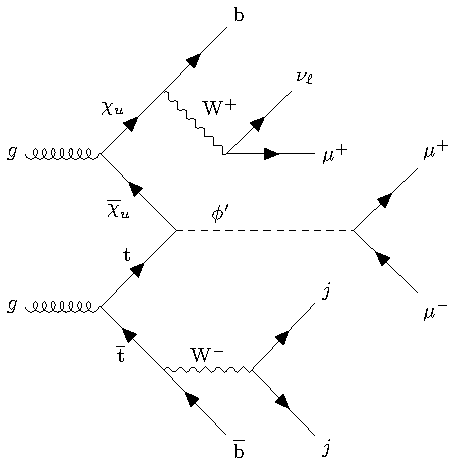
\includegraphics[width=0.85\linewidth]{Images/signal_qqfusion.pdf}
    \caption{Representative Feynman diagram for the production of a $\phi'$ boson in association with a $\chi_\mathrm{u}$ vector-like quark through the fusion of a top quark and $\chi_\mathrm{u}$ vector-like quark. Once again, the $\phi'$ decays to a pair of muons, the top quark decays fully hadronically, and the $\chi_\mathrm{u}$ decays semi-leptonically to muons, neutrinos and $b$-jets.\label{fig:qqfusion}}
\end{figure}

\begin{figure}
    \centering
    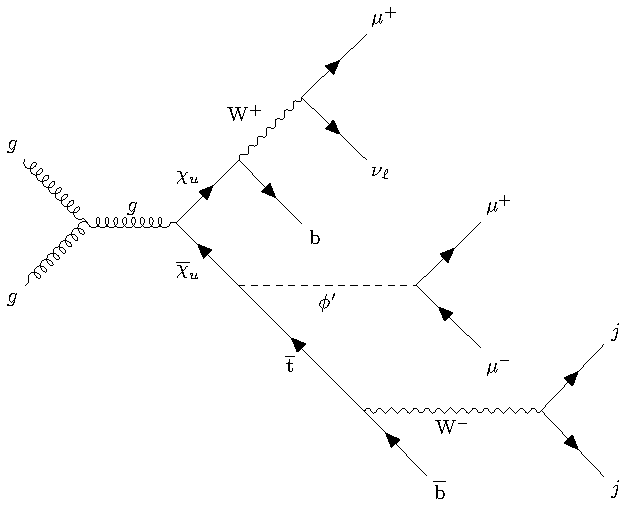
\includegraphics[width=0.85\linewidth]{Images/signal_ggfusion.pdf}
    \caption{Representative Feynman diagram for the production of a $\phi'$ boson in association with a $\chi_\mathrm{u}$ vector-like quark through the fusion of a gluon pair from incoming protons. The $\phi'$ decays to a pair of muons, the top quark that decays fully hadronically, and the $\chi_\mathrm{u}$ decay semi-leptonically to muons, neutrinos and jets.\label{fig:ggfusion}}
\end{figure}

\section{Experimental Considerations}\label{sec:exp}

The ATLAS and CMS collaborations at CERN have conducted various searches for heavy vector-like quarks (T). These searches utilized $\mathrm{pp}$ collisions at center-of-mass energies of $\sqrt{s} = 8$ and $13$ \textrm{TeV}. The studies primarily focused on T production through gluon-mediated QCD processes, either in pair production from quark-antiquark annihilation (Figure~\ref{fig:qcd_T_prod}) or in single-T production from electroweak processes involving associated quarks (Figure~\ref{fig:qed_T_prod}). 

\begin{figure}
\centering
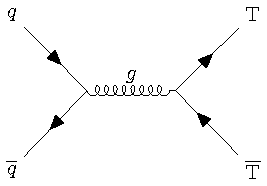
\includegraphics[width=0.65\linewidth]{Images/T_prod_qcd.pdf}
\caption{Representative Feynman diagram for T pair production via gluon-mediated QCD processes.\label{fig:qcd_T_prod}}
\end{figure}

\begin{figure}
\centering
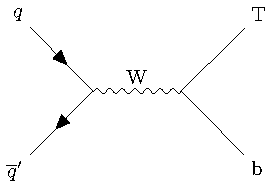
\includegraphics[width=0.65\linewidth]{Images/T_prod_qed.pdf}
\caption{Representative Feynman diagram for single T production via electroweak processes.\label{fig:qed_T_prod}}
\end{figure}


In those studies, \textrm{T} decays into $\mathrm{bW}$, $\mathrm{tZ}$, or $\mathrm{tH}$ have been considered. In the context of \textrm{T} pair production, $\mathrm{T}\bar{\mathrm{T}}$, via QCD processes, the cross sections are well-known and solely depend on the mass of the vector-like quark.  Assuming a narrow $\mathrm{T}$ decay width ($\Gamma / m(\mathrm{T}) < 0.05$ or 0.1) and a 100\% branching fraction to $\textrm{bW}$, $\textrm{tZ}$, or $\textrm{tH}$, these searches have set stringent bounds on $m(\mathrm{T})$, excluding masses below almost 1.5 \textrm{TeV} at 95\% confidence level~\parencite{CMS:2024bni,CMS:2024qdd,ATLAS:2022ozf,ATLAS:2023bfh,ATLAS:2022hnn,ATLAS:2022tla,ATLAS:2023pja,ATLAS:2024fdw}. The most recent analysis from the CMS collaboration probes T-quark production via $\mathrm{pp} \to \mathrm{T}\textrm{qb}$, in final states with $\mathrm{T} \to \textrm{tZ}$ or $\mathrm{T} \to \textrm{tH}$, considering scenarios with preferential couplings to third-generation fermions. The analysis sets 95\% confidence level upper limits of 68-1260 \textrm{fb} on the production cross section, for T masses ranging from 600-1200 \textrm{GeV}~\parencite{CMS:2024qdd}. The latest studies from ATLAS probe vector-like quarks using the single-T production mode with the $\mathrm{T} \to \textrm{tH}$ decay channel leading to a fully hadronic final state~\parencite{ATLAS:2022ozf}, the single-T production mode with the $\mathrm{T} \to \textrm{tZ}$ decay channel leading to a multileptonic final state~\parencite{ATLAS:2023bfh}, the TT pair production mode with various T decay channels leading to multileptonic final states~\parencite{ATLAS:2022hnn}, and the TT pair production mode with various T decay channels leading to a single lepton plus missing momentum final state~\parencite{ATLAS:2022tla,ATLAS:2023pja}. 
The multilepton search offers the greatest sensitivity in most of the phase space, but the missing transverse energy based search has better sensitivity for low branching fraction $\mathfrak{B}(\mathrm{T}\to \textrm{Wb})$ and high $\mathfrak{B}(\mathrm{T}\to \textrm{Ht})$. These searches have similar sensitivities for the singlet and doublet models, resulting in exclusion bounds for masses below about 1.25 \textrm{TeV} and 1.41 \textrm{TeV}, respectively. 


A key consideration in the model interpretations summarized above is that the $\mathrm{T}$ branching fractions depend on the chosen model. The excluded mass range is less restrictive for specific branching fraction scenarios, such as $\{\mathfrak{B}(\mathrm{T} \to \textrm{tZ})$, $\mathfrak{B}(\mathrm{T} \to bW)$, $\mathfrak{B}(\mathrm{T} \to \textrm{tH})\}= \{0.2, 0.6, 0.2\}$, excluding masses below about 0.95 \textrm{TeV}. Moreover, if the $\mathrm{T} \to \phi't $ decay is allowed, or if the branching fractions $\mathfrak{B}(\mathrm{T} \to \textrm{tH/bW})$ are lower, the limits previously quoted must be re-evaluated. The authors of Ref.~\parencite{Cacciapaglia:2019zmj} emphasize that bounds on $m(\mathrm{T})$ can be around 500 \textrm{GeV} when $\mathrm{T} \to \mathrm{t}\phi'$ decays are permitted. Therefore, to facilitate a comprehensive study, benchmark scenarios in this paper are considered down to $m(\chi_\mathrm{u}) = 500$ \textrm{GeV}.

\section{\boldmath The Minimal $U(1)_{T_R^3}$ Model}\label{sec:model}
\subsection{Scalar Potential}
In this model, the SM is extended by the Abelian gauge symmetry $U(1)_{T^3_R}$, where only right-handed fermions are charged. We assume two independent Higgs mechanisms, one with a Higgs doublet $\mathrm{H}$ for electroweak symmetry breaking and the other with a Higgs singlet $\phi$ for the $U(1)_{T^3_R}$ symmetry breaking. Both scalars have independent vacuum expectation values (VEVs), $\expval{H}=v_h/\sqrt2$ and $\expval\phi =v_\phi/\sqrt2$, allowing us to express the doublet and singlet Higgs fields, following a Kibble parametrization, as 
\begin{align}
    H & = \begin{pmatrix}
        G_{+} \\
        \frac{1}{\sqrt{2}}\left(v_h+\rho_0+i G_{0}\right)
    \end{pmatrix}\label{eq:higgskibblepara1}
    \\
    \phi & =\frac{1}{\sqrt{2}}\left(v_\phi + \rho_\phi+i G_{\phi}\right). \label{eq:higgskibblepara2}
\end{align}
In Eqs.\ref{eq:higgskibblepara1} and Eq.\ref{eq:higgskibblepara2}, $G_\pm$, $G_0$, and $G_\phi$ are the Goldstone bosons that allow the SM $\textrm{W}^\pm$ and $\textrm{Z}$ bosons and the dark photon $A'$, associated with the $U(1)_{T^3_R}$ symmetry, to acquire mass. The $\rho_h$ and $\rho_\phi$ are an orthogonal mixture of the SM Higgs boson and the dark Higgs
\begin{equation}
    \begin{pmatrix}
        h
        \\
        \phi'
    \end{pmatrix}
    =
    \begin{pmatrix}
        \cos\alpha & -\sin\alpha
        \\
        \sin\alpha & \cos\alpha
    \end{pmatrix}
    \begin{pmatrix}
        \rho_0
        \\
        \rho_\phi
    \end{pmatrix},
\end{equation}
that results from the diagonalization of the mass matrices arising from the gauge invariant potential
\begin{equation}
    \begin{aligned}
        \mathcal V(\phi,H)
    &= \mu_H^2 H^{\dagger} H 
    +\mu_\phi^2 \phi^* \phi
    \\
    &+\lambda\left(H^{\dagger} H\right)\left(\phi^* \phi\right)
    +\lambda_H\left(H^{\dagger} H\right)^2
    +\lambda_\phi\left(\phi^* \phi\right)^2.
    \end{aligned}
\end{equation}
The tadpole equations are given from the minimization of the potential as
\begin{align}
    \pdv{\mathcal V}{H} 
     &= \frac{v_h}{\sqrt2} \left( \mu_H^2 +\lambda_Hv_h^2 + \frac{1}{2} \lambda v_\phi^2 \right) = 0,
    \\
    \pdv{\mathcal V}{\phi}
    &= \frac{v_\phi}{\sqrt2} \left( \mu_\phi^2 +\lambda_\phi v_\phi^2 + \frac{1}{2} \lambda v_h^2 \right) = 0.
\end{align}
The masses of the scalar bosons can be written as
\begin{equation}
    \begin{aligned}
        m_{h,\phi'}^2 &= \frac{1}{2}\left( 
    \lambda_H v_h^2 + \lambda_\phi v_\phi^2
    \right)\\
    &\pm 
    \sqrt{
        \lambda^2 v_h^2 v_\phi^2
        +
        \left(
        \lambda_H v_h^2 - \lambda_\phi v_\phi^2
        \right)^2
    },
    \end{aligned}
\end{equation}
and the mixing angle $\alpha$ as
\begin{equation}
    \tan \alpha = \frac{-\lambda v_h v_\phi}{ \lambda_H v_h^2 - \lambda_\phi v_\phi^2 - \sqrt{\lambda^2 v_h^2 v_\phi^2 + \left(\lambda_H v_h^2 - \lambda_\phi v_\phi^2\right)^2}}.
\end{equation}

\subsection{The Universal Seesaw Mechanism}
In the model, each electrically charged SM fermion $f$ has a mass protected by both VEVs. In turn, they  acquire mass from the mixture with a vector-like fermion $\chi_f$, which is charged as the right-handed component of the respective SM fermion, in a UV complete theory. The terms in the Lagrangian density that contribute to the mass of physical fermions are,
\begin{equation}
    \begin{aligned}
        -\mathcal{L}&\supset 
    Y_{f_L} \bar{f}_L' \chi_{fR}' H 
    +Y_{f_R} \bar\chi_{fL}' f'_R  \phi^* 
    + m_{\chi_f'} \bar{\chi}_{f L}' \chi_{f R}'\\
&+\text { h.c.}
    \end{aligned}
\end{equation}
Therefore, in the vacuum, the mass matrix is
\begin{equation}
    M_f=
    \begin{pmatrix}
    0 & Y_{f_L} v_h /\sqrt2\\
    Y_{f_R} v_\phi /\sqrt2 & m_{\chi_f'}    
    \end{pmatrix}.
\end{equation}
The left- and right-handed components of the physical fermions $(f,\,\chi_f)$ are given by two rotations $\mathcal R(\theta_{f_{L,R}})$ as, 
\begin{equation}
    \begin{pmatrix}
        f_{L,R}
        \\
        \chi_{f_{L,R}}
    \end{pmatrix}
    =
    \begin{pmatrix}
        \pm\cos\theta_{f_{L,R}} & \mp \sin \theta_{f_{L,R}}
        \\
        \sin \theta_{f_{L,R}} & \cos\theta_{f_{L,R}}
    \end{pmatrix}
    \begin{pmatrix}
        f_{L,R}'
        \\
        \chi_{f_{L,R}}'
    \end{pmatrix},
\end{equation}
in a way that $\mathcal{R}(\theta_{f_L})M_f\mathcal{R}^{-1}(\theta_{f_R})=\text{diag}(m_f,m_{\chi_f})$ up to a phase. Assuming real parameters, the physical masses and the mixing angles are given by
\begin{gather}
    m_f m_{\chi_f}=\frac{ \left(Y_{f_{L}} v_h\right) \left(Y_{f_R} v_\phi\right)}{2}, \label{eq:prodmass}
     \\ 
    m_f^2 + m_{\chi_f}^2 = m_{\chi_f'}^2 + \frac{1}{2}\left(Y_{f_L}^2v_h^2+Y_{f_R}^2v_\phi^2\right),\label{eq:summass}
    \\
    \tan \theta_{f_{L,R}} =  \frac{\sqrt 2}{m_{\chi_f'}}\left(\frac{Y_{f_{L,R}}v_{h,\phi}}{2} - 
    \frac{m_f^2}{Y_{f_{L,R}}v_{h,\phi}} \right).
\end{gather}

\noindent The Yukawa interactions of the physical fermions with the scalar bosons have the form
\begin{equation}
    -\mathcal{L}_{\text{yuk}} 
    = h \bar\psi_{f_L} \mathcal{Y}_{h}\psi_{f_R} + \phi' \bar\psi_{f_L} \mathcal{Y}_{\phi}\psi_{f_R},
\end{equation} 
with $\psi_{f} = (f,\chi_{f})^T$, and the matrices $\mathcal{Y}_{f_{L,R}}$ given by
\begin{align}
    \mathcal{Y}_{h} &= \frac{1}{\sqrt{2}}
    \mathcal{R}(\theta_{f_L})
    \left(
        Y_{f_L}\sigma_+ \cos\alpha 
    - 
    Y_{f_R}\sigma_-\sin\alpha
    \right)
    \mathcal{R}^{-1}(\theta_{f_R})\label{eq:YukawaL}
    \\
    \mathcal{Y}_{\phi} &= \frac{1}{\sqrt{2}}
    \mathcal{R}(\theta_{f_L})
    \left(
    Y_{f_L}\sigma_+ \sin\alpha
    +
    Y_{f_R}\sigma_-\cos\alpha
    \right)
    \mathcal{R}^{-1}(\theta_{f_R}),\label{eq:YukawaR}
\end{align}
where $\sigma_{\pm}=(\sigma_1\pm i\sigma_2)/2$ are the ladder Pauli matrices.

\subsection{Minimal UV-complete theory}

The model must provide non-zero masses for all the SM fermions and be free of gauge anomalies. So, we must have at least one full generation of vector-like fermions $\{\chi_\mathrm{u}$, $\chi_\mathrm{d}$, $\chi_\mathrm{\ell}$, $\chi_\mathrm{\nu}\}$ and the right-handed component of the SM neutrinos, $\nu_R$, charged as shown in Table~\ref{tab:QMnumbers}. Therefore, the Yukawa interactions in the UV-complete theory must be of the form
\begin{equation}
    \begin{aligned}
        -\mathcal{L}
        \supset&\quad
        Y_{L u}^i \bar{q}_L^{\prime i} \chi_{u R}' \widetilde{H}
        + Y_{R u}^i \bar{\chi}_{u L}' u_R^{\prime i} \phi^*  
        + m_{\chi_\mathrm{u}} \bar{\chi}_{u L}' \chi_{u R}'
        \\&
        +Y_{L d}^i \bar{q}_L^{\prime i} \chi_{d R}' H 
        +Y_{R d}^i \bar{\chi}_{d L}' d_R^{\prime i} \phi
        +m_{\chi_d} \bar{\chi}_{d L}' \chi_{d R}'
        \\&
        +Y_{L \ell}^{i} \bar{\ell}_L^{\prime i} \chi_{\ell R}' H
        +Y_{R \ell}^{i} \bar{\chi}_{\ell L}' \ell_R^{\prime i} \phi
        +m_{\chi_\ell} \bar{\chi}_{\ell L}' \chi_{\ell R}'
        \\
        &
        +Y_{L \nu}^{i} \bar{\ell}_L^{\prime i} \chi_{\nu R}' \widetilde{H}
        +Y_{R \nu}^{i} \bar{\chi}_{\nu L}' \nu_R^{\prime i} \phi^*
        +m_{\chi_\nu} \bar{\chi}_{\nu L}' \chi_{\nu R}' \\
        &+\text { h.c., }
    \end{aligned}
\end{equation}
where the $i$ index runs over the three generations of fermions. The simultaneous diagonalization of the mass matrices of each fermion sector will have a similar structure to the one presented in Eqs.~\ref{eq:prodmass} and~\ref{eq:summass} and the Yukawa matrices will have a similar structure of Eqs.~\ref{eq:YukawaL} and~\ref{eq:YukawaR} but codifying the $CKM$ matrix. For the neutrino sector, the structure of the mass matrix will be more complicated due to the presence of the additional Majorana mass term for the vector-like neutrino $\chi_\nu'$.

\begin{table}[h]
    \centering
    \begin{tabular}{ccccc}
    \hline
    \hline
        Field & $SU(3)_C$  & $SU(2)_L$ & $U(1)_Y$ & $U(1)_{T^3_R}$ \\
    \hline\hline
        $q_L'$                    & \bf{3} & \bf{2} & 1/6 & 0\\
        $\ell_L'$                 & \bf{1} & \bf{2} & -1/2 & 0\\
        $H$                         & \bf{1} & \bf{2} & 1/2 & 0\\
        \hline
        $u_R^{\prime c}$          & \bf{3} & \bf{1} & -2/3 & -2\\
        $d_R^{\prime c}$          & \bf{3} & \bf{1} & 1/3 & 2\\
        $\ell_R^{\prime c}$       & \bf{1} & \bf{1} & 1 & 2\\
        $\nu_R^{\prime c}$        & \bf{1} & \bf{1} & 0 & -2\\
        $\phi$                      & \bf{1} & \bf{1} & 0 & 2\\
        \hline
        $\chi_{u_L}'$               & \bf{3} & \bf{1} & 2/3 & 0\\
        $\chi_{u_R}^{\prime c}$     & \bf{3} & \bf{1} & -2/3 & 0\\
        $\chi_{d_L}'$               & \bf{3} & \bf{1} & -1/3 & 0\\
        $\chi_{d_R}^{\prime c}$     & \bf{3} & \bf{1} & 1/3 & 0\\
        $\chi_{\ell_L}'$            & \bf{1} & \bf{1} & -1 & 0\\
        $\chi_{\ell_R}^{\prime c}$  & \bf{1} & \bf{1} & 1 & 0\\
        $\chi_{\nu_L}'$             & \bf{1} & \bf{1} & 0 & 0\\
        $\chi_{\nu_R}^{\prime c}$   & \bf{1} & \bf{1} & 0 & 0\\
    \hline
    \hline
    \end{tabular}
    \caption{Minimal field content of the model and their representations under the SM and $U(1)_{T^3_R}$ gauge groups.}
    \label{tab:QMnumbers}
\end{table}

\section{Samples and Simulation}\label{sec:sims}
The minimal $U(1)_{T^3_R}$ model described in Sec.~\ref{sec:model} is implemented into the \texttt{FeynRules} package~\parencite{Alloul:2013bka}, which generates the Feynman rules and exports them into a Universal \texttt{FeynRules} Output (\texttt{UFO})~\parencite{Degrande:2011ua}. The resulting \texttt{UFO} is utilized as input for a generator to produce the MC samples. Both signal and background events are generated with the \texttt{MadGraph5\_aMC@NLO} v3.2.0 program~\parencite{Alwall:2014hca,Alwall:2014bza} at leading order (LO) in QCD, considering \textrm{pp} beams colliding with a center-of-mass energy of $\sqrt{s} = 13.6$ \textrm{TeV}. Each signal and background sample is generated separately, with no interference effects between the signal and background considered. The impact of these interference effects has been evaluated, and for all values of $\chi_\mathrm{u}$ and $\phi'$ masses considered, the effect on the signal plus background cross section is found to be less than $<0.5$\%. Additionally, the effect on the shape of the b-jet $p_{T}$ distribution is less than 6\% for $p_{T} < 300$ GeV and less than 2\% for b-jet $p_{T} > 300$ GeV. We use the \texttt{NNPDF3.0~NLO}~\parencite{NNPDF:2014otw} set for parton distribution functions (PDFs) for all event generation. Parton-level events are then interfaced with \texttt{PYTHIA} (v8.2.44)~\parencite{Sjostrand:2014zea} to account for parton showering and hadronization processes. Finally, we use  \texttt{DELPHES} (v3.4.2)~\parencite{deFavereau:2013fsa} to simulate smearing and other detector effects using the CMS detector geometric configurations and parameters for particle identification and reconstruction, using the CMS input card with 140 average pileup interactions. All signal cross sections used in this analysis are obtained requiring the following kinematic criteria on leptons $\ell$, \textrm{b} quarks, and light-quark/gluon jets ($j$) at parton level in \texttt{MadGraph}: $p_{\mathrm{T}}(\ell) > 35$~\textrm{GeV}, $\abs{\eta (\mathrm{b})} < 2.5$, $\abs{\eta (\ell)} < 2.3$, $p_{\mathrm{T}}(j) > 20$~\textrm{GeV}, and $\abs{\eta (\mathrm{j})} < 5$. These parton-level selections were applied exclusively to the signal processes to restrict event generation to the relevant phase space regions. For background processes, these default parton level requirements in \texttt{MadGraph} were imposed:  $p_{\mathrm{T}}(\ell) > 10$~\textrm{GeV}, $\abs{\eta (\ell)} < 2.5$, $p_{\mathrm{T}}(j) > 20$~\textrm{GeV}, $\abs{\eta (\mathrm{j})} < 5$, and $\abs{\eta (\mathrm{b})} < 5$. This ensures that the phase space regions for the background near the analysis-level selection criteria are adequately described after parton showering since the pre-selections at the analysis level are more stringent than the parton-level requirements. Furthermore, we use the MLM algorithm for jet matching and jet merging. The parameters \texttt{xqcut} and \texttt{qcut} of the MLM algorithm are set to 30 and 45 respectively to ensure continuity of the differential jet rate as a function of jet multiplicity. Each simulated signal and background sample is produced separately at LO, with one million events at the generation level, neglecting potential interference effects between the signal and background due to the suppression caused by the different orders of magnitude in the coupling constants of the signal and background.

Signal samples are generated considering the production of a $\phi'$ boson, an associated $\chi_\mathrm{u}$ vector-like quark, and a top quark $(\mathrm{pp}\to \chi_\mathrm{u} \mathrm{t} \phi')$, inclusive in both $\alpha$ and $\alpha_s$ (see Figures~\ref{fig:qqfusion}-\ref{fig:ggfusion}). We have used the implementation of the $U(1)_{T^3_R}$ model in Ref.~\parencite{Dutta2023}. Signal samples were created considering coupling values of $Y_{\mathrm{t}_R}=Y_{\mathrm{t}_L}=2\sqrt{2}$ in the range of masses $m(\phi')\in\{5,10,50,100,325\}$~\textrm{GeV} for the dark higgs and $m(\chi_\mathrm{u})\in\{0.50, 0.75, 1.0, 1.5, 2.0, $ $ 2.5\}$~\textrm{TeV} for the vector-like quark $\chi_u$~\parencite{PhysRevD.108.095006}. The production cross section for $\mathrm{pp}\to \chi_\mathrm{u} \mathrm{t} \phi'$ is highly dependent on the choice of the Yukawa couplings in the Lagrangian. The ${\chi_\mathrm{u}}{- \mathrm{t}}$ fusion process shown in Figure~\ref{fig:qqfusion} is dominated by the $Y_{\mathrm{t}_R}$ coupling. However, the decay ${\chi_\mathrm{u}} \to \mathrm{t} \phi'$ shown in Figure~\ref{fig:ggfusion} is inversely proportional to the $Y_{\mathrm{t}_L}$ coupling. This effect is shown in Figure~\ref{fig:cross_section_by_lambdas}, which displays the total signal cross section, as a function of $Y_{\mathrm{t}_R}$ and $Y_{\mathrm{t}_L}$, for a benchmark point with $m(\phi')=100$~\textrm{GeV} and $m(\chi_\mathrm{u})=1.0$~\textrm{TeV}. 

\begin{figure}
    \centering
    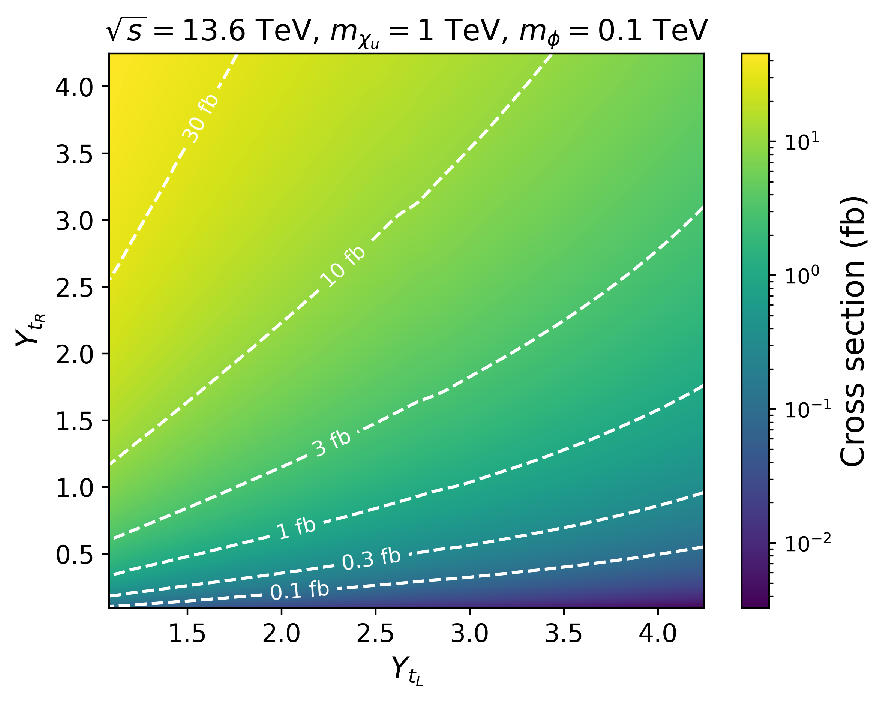
\includegraphics[width=0.85\linewidth]{Images/cross_section_by_lambdas.pdf}
    \caption{Signal production cross section, $ \mathrm{pp}\to \chi_\mathrm{u} \mathrm{t} \phi'$,  in the $Y_{\mathrm{t}_R}$ versus $Y_{\mathrm{t}_L}$ plane, for a benchmark point with $m(\phi')=100$~\textrm{GeV} and $m(\chi_\mathrm{u})=1.00$~\textrm{TeV}. The white-dashed contours show specific cross section values in the two dimensional plane.}
    \label{fig:cross_section_by_lambdas}
\end{figure}

We target signal events where the top quark decays hadronically into a bottom quark and two jets ($\mathrm{t} \to \mathrm{bW} \to \mathrm{b} q \bar{q}'$), the $\chi_\mathrm{u}$ decays semileptonically into a $b$ quark, lepton, and neutrino (via $\chi_\mathrm{u} \to \mathrm{bW}$ and $\mathrm{W}\to\mu\nu_{\mu}$), and the $\phi'$ produces two muons. We note that the scalar $\phi'$ particle could result from the mixture of the SM Higgs boson and additional scalar fields, and the Yukawas of the fermions could additionally arise from the mixing of the SM fermions with additional copies of the associated vector-like fermions. Therefore, the $\phi'$ branching ratios are dependent on the chosen mechanism and model by which this mixture occurs, see for example, Refs.~\parencite{Cacciapaglia_2023,Blankenburg:2012nx,Jones-Perez:2013oia,Calibbi:2009pv}. For the purpose of this work, and 
similar to Refs.~\parencite{Dutta2020,Dutta2023}, the considered benchmark signal scenarios have $\mathfrak{B}(\chi_\mathrm{u} \rightarrow \textrm{b W})$ of about 0.5 and $\mathfrak{B}(\phi' \rightarrow \mu^+\mu^-)=0.98$. Figure~\ref{fig:xs-plot} shows the production cross section in \textrm{fb}, as a function of $m(\phi')$ and $m(\chi_\mathrm{u})$ masses, assuming the aforementioned decays, branching ratios, and couplings.

We note that for the parameter space of focus in this paper, the total mass of the $t$-$\chi_\mathrm{u}$ system is larger than $m(\phi')$, thus the large rest energy of the $t$-$\chi_\mathrm{u}$ system is converted into potentially large momentum values for the $\phi'$. Similarly, the $t$-quark produced through the $\chi_\mathrm{u}$-$t$ fusion interaction can also have large momentum values, and thus in some cases the hadronic $t$ decay products cannot be fully reconstructed independently of each other. This results in three possible $t$ reconstruction scenarios: a fully merged scenario where the $\mathrm{W}\to jj$ system and the $\mathrm{b}$ quarks are very collimated and reconstructed as a single ``fat jet’’ (henceforth referred to as a FatJet, FJ); a partially merged scenario, where the decay products of the $\mathrm{W}$ boson form a single FatJet but the $\mathrm{b}$ quark can still be separately identified; and an un-merged scenario where all decay products can be independently identified. Jets are clustered using the anti-$k_t$ algorithm~\parencite{Cacciari_2008} using the \texttt{FastJet} (v3.4.2)~\parencite{Cacciari_2012} package with a distance parameter of $R = 0.4$ for standard jets and $R = 0.8$ for fat jet objects. Each scenario has an associated identification efficiency and misidentification rate, which depends on the choice of the boosted $t$/$W$ algorithm (our choice of efficiency and misidentification rates is described later). 

Based on the above details, the final state of interest in this paper consists of three muons (two from the $\phi'$ decay and one from the $\chi_\mathrm{u}$ decay), a (possibly boosted) top-tagged system, at least one $b$-tagged jet, and large missing transverse momentum ($\vec{p}_{T}^{\textrm{~miss}}$). For the partially merged and un-merged scenarios, there will be two $b$ quarks present in the final state (one of which is part of the top tagged system). 

We consider background sources from SM processes which can give similar objects in the final state as those expected for signal. Several background sources were considered and studied, such as QCD multijet events, production of vector boson pairs ($\mathrm{VV: WW, ZZ, WZ}$), vector boson triplets ($\mathrm{VVV: WWZ, WZZ, ZZZ, WWW}$), top-quark pairs in association with weak bosons ($\mathrm{t}\overline{\mathrm{t}}X$), and $\mathrm{t}\overline{\mathrm{t}}\mathrm{t}\overline{\mathrm{t}}$ processes. The  dominant sources of SM background events are from the $\mathrm{t}\overline{\mathrm{t}}X$, $\mathrm{ZZW}$, and $\mathrm{t}\overline{\mathrm{t}}\mathrm{t}\overline{\mathrm{t}}$ processes. The $\mathrm{t}\overline{\mathrm{t}}X$ background is primarily associated production of a $\mathrm{Z}/\gamma^{*}$ from $\mathrm{t}\bar{\mathrm{t}}$ fusion processes. The $\mathrm{ZZW}$ process becomes a background when one $\mathrm{Z}$ decays $\mathrm{b}\bar{\mathrm{b}}$, another $\mathrm{Z}$ decays to a pair of muons, and the W decays to a muon and a neutrino. 
Events from $\mathrm{ZZW}$ and $\mathrm{t}\overline{\mathrm{t}}\mathrm{t}\overline{\mathrm{t}}$ have been combined, after being weighted by their corresponding production cross section. The combination is presented as the ``$\mathrm{b} \overline{\mathrm{b}}\mu\mu\mu\nu$'' background in the remainder of this paper. The $\mathrm{t}\overline{\mathrm{t}}X$ process is presented as part of the ``$\mathrm{t}\overline{\mathrm{t}}\mu^{+}\mu^{-}$'' background. Table~\ref{tab:dominantbkgs} shows the production cross sections for the dominant background sources. The rest of the aforementioned background processes do not contribute meaningfully in our context, accounting for $\ll 1\%$ of the total expected background yield.

The identification of leptons, boosted top quarks, and bottom quarks plays an important role in the ability to identify signal events, the ability to minimize the rate of SM backgrounds, and thus also the discovery reach in the high-luminosity environment of the LHC. It is worth noting that the reconstruction and identification of leptons and the decay products of the top/bottom quarks may be non-trivial at the High-Luminosity LHC (HL-LHC) due to the presence of a potentially large number of secondary pp interactions (pileup). The impact of pileup on the new physics discovery reach, and the importance of pileup mitigation at CMS and ATLAS has been outlined in many papers, for example in Ref.~\parencite{CMS-PAS-FTR-13-014}. We note the expected performance of the upgraded ATLAS and CMS detectors for the HL-LHC is beyond the scope of this work; however, the studies presented here do attempt to provide reasonable expectations by conservatively assuming some degradation in lepton and hadron identification efficiencies, using Ref.~\parencite{CMS-PAS-FTR-13-014} as a benchmark, and considering the case of 140 average pileup interactions. 

For muons with $|\eta|< 1.5$, the assumed identification efficiency is 95\% with a 0.3\% misidentification rate~\parencite{CMS-PAS-FTR-13-014,CMS_MUON_17001}. The performance degrades linearly with $\eta$ for $1.5 < |\eta| < 2.5$, and we assume an identification efficiency of 65\% with a 0.5\% misidentification rate at $|\eta| = 2.5$. Similarly, the charged hadron tracking efficiency, which contributes to the jet clustering algorithm and missing transverse momentum ($\vec{p}_{T}^{\textrm{~miss}}$) calculation, is 97\% for $1.5 < |\eta| < 2.5$, and degrades to about 85\% at $|\eta| = 2.5$. These potential inefficiencies due to the presence of secondary pp interactions contribute to how well the lepton and top kinematics can be reconstructed. Following Refs.~\parencite{CMS:2020poo,ATLAS:2018wis}, we consider the ``Loose'' working point for the identification of the fully merged (partially merged) $\mathrm{t}$ decays, which results in 80-85\% top (W) identification efficiency and 11-25\% misidentification rate, depending on the FatJet transverse momentum ($p_{T}^{FJ}$). Following Ref.~\parencite{CMSbtag}, we consider the ``Loose'' working point of the DeepCSV algorithm~\parencite{Bols_2020}, which gives a 70-80\% b-tagging efficiency and 10\% light quark mis-identification rate. The choice of boosted $t$/$W$ and b-tagging working points is determined through an optimization process that maximizes discovery reach. It is noted the contribution from SM backgrounds with a misidentified boosted $t$/$W$ is negligible, and thus our discovery projections are not sensitive to uncertainties related to the boosted $t$/$W$ misidentification rates. 

\begin{figure}
    \centering
    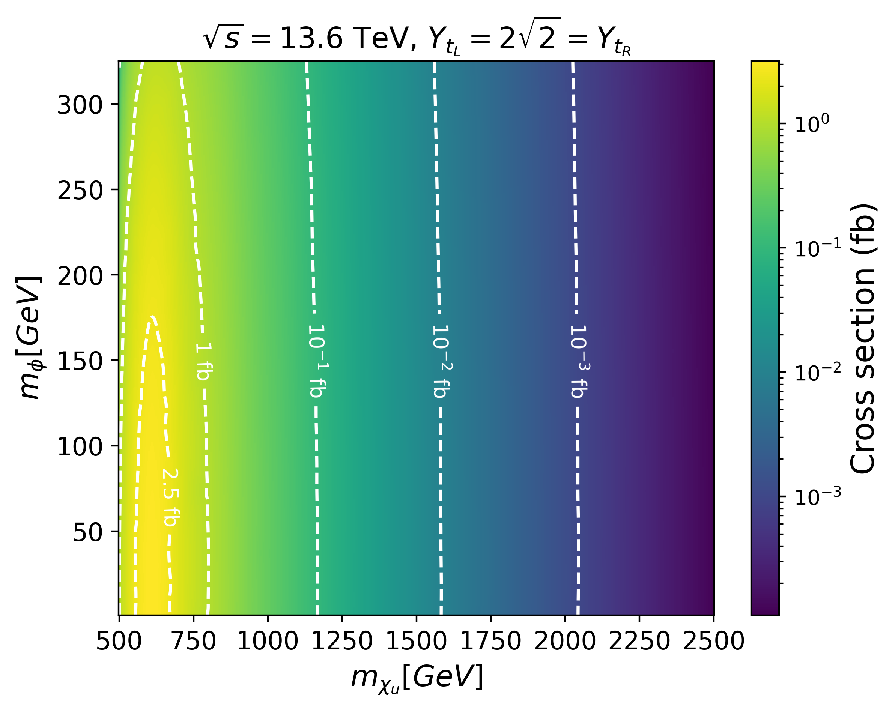
\includegraphics[width=0.85\linewidth]{Images/cross_section_by_masses.pdf}
    \caption{Projected cross section (fb) plot for $pp\to t \chi_\mathrm{u} \phi'$ and subsequent decay as a function of $m(\chi_\mathrm{u})$ and $m(\phi')$.}
    \label{fig:xs-plot}
\end{figure}

\begin{table}[]
  \begin{tabular}{l r}
    \hline
    {Background Process} & {Cross-Section $\sigma$ [\textrm{pb}]} \\
    \hline
   $\mathrm{pp} \to \mathrm{t} \overline{\mathrm{t}} \, \mu^+ \mu^-$ & $2.574\times 10^{-3}$  \\
    $\mathrm{pp} \to \mathrm{b}\overline{\mathrm{b}}\, \mu\mu\mu\nu $ & $4.692 \times 10^{-4}$ \\
    \hline
  \end{tabular}
  \centering
  \caption{A summary of dominant SM backgrounds produced by $\mathrm{pp}$ collisions and their cross sections in pb, as computed by \texttt{MadGraph} with $n = 10^6$ events.}
  \label{tab:dominantbkgs}
\end{table}

\begin{figure}[]
\centering
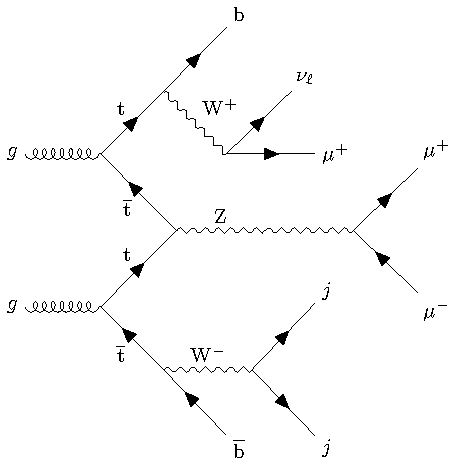
\includegraphics[width=.75\linewidth]{Images/bg_Z_full.pdf}
\caption{Representative Feynman diagram for a background event. A $Z$ boson is produced in association with a top quark through the fusion of a top, anti top pair from incoming protons. The $Z$ boson subsequently decays to a pair of muons and the two spectator top quarks decay semi-leptonically and purely hadronically to muons, neutrinos and jets, resulting in the same final states as the signal event.\label{fig:v}}
\end{figure}

\section{Data Analysis Using Machine Learning}\label{sec:ML}
The analysis of signal and background events is performed utilizing machine learning techniques. A machine learning-based approach offers sizeable advantages when compared to traditional event classification techniques. Unlike conventional methods, machine learning models have the capability to simultaneously consider all kinematic variables, allowing them to efficiently navigate the complex and high-dimensional space of event kinematics. Consequently, machine learning models can effectively enact sophisticated selection criteria that take into account the entirety of this high-dimensional space. This makes them ideal for high-energy physics applications.

The BDT method is a powerful machine learning technique that has proven its effectiveness in various applications, particularly in the field of collider physics. In this method, decision trees are trained greedily in a sequential manner, with each tree focusing on learning the discrepancies or residuals between its predictions and the expected values obtained from the previously trained tree. This iterative process aims to progressively minimize errors, making BDTs a particularly effective approach for enhancing model performance.

In the context of collider physics, BDTs have demonstrated their utility in addressing classification problems. In particular, BDTs can effectively discriminate between signal and background events, enabling accurate and efficient event classification. Their ability to handle subtle non-linear relationships within the data with high interpretability makes BDTs a valuable tool to handle large amounts of data with a large number of parameters for each event. 

The first step in our workflow involves the use of a specialized \texttt{MadAnalysis Expert Mode} C++ script~\parencite{CONTE2013222}. This script extracts essential kinematic and topological information from the simulated samples. The script will process the aforementioned variables contained within these files and transform them into a structured and informative CSV (Comma-Separated Values) format that can be used to train our machine learning models. These kinematic variables include crucial details about the events, such as particle momenta, energies, and topologies, providing the fundamental building blocks for our machine learning analysis. Figure~\ref{fig:feature_importance} shows the features that are used for training the machine learning models and their importance for a benchmark point.

To account for the differential significance of various events, we apply cross-section weighting. This ensures that the relative importance of signal and background events is appropriately balanced in the dataset. This weighting is crucial for addressing the varying likelihood of observing different types of events in high-energy physics experiments. The prepared and weighted datasets are then passed to our \texttt{MadAnalysis Expert Mode} C++ script, where the simulated signal and background events are initially filtered, before being passed to the CSV file for use by the machine learning algorithm. The filtering process requires at least one well-reconstructed and identified $\mathrm{b}$-jet candidate, at least one jet (regular or FJ) not tagged as a $\mathrm{b}$ jet, and exactly three identified muons. The filtering selections are motivated by experimental constraints, such as the geometric constraints of the CMS/ATLAS detectors, the typical kinematic thresholds for the reconstruction of particle objects, and the available lepton triggers which also drive the minimal kinematic thresholds. Selected jets must have $p_{\mathrm{T}} > 30$ $\textrm{GeV}$ and $|\eta(j)| < 5.0$, while $\mathrm{b}$-jet candidates with $p_{\mathrm{T}} > 20$ $\textrm{GeV}$ and $|\eta(\mathrm{b})| < 2.5$ are chosen. The $\mu$ object must pass a $p_{\mathrm{T}} > 35$ $\textrm{GeV}$ threshold and be within a $|\eta(\ell)| < 2.3$. We will refer to this filtering criteria as pre-selections. The efficiency of the pre-selections depends on $m(\phi')$ and $m(\chi_{\mathrm{u}})$, but is typically about 25-30\% for the signal samples. Events passing this pre-selection are used as input for the machine learning algorithm, which classifies them as signal or background, using a probability factor. 

\begin{figure}
\centering
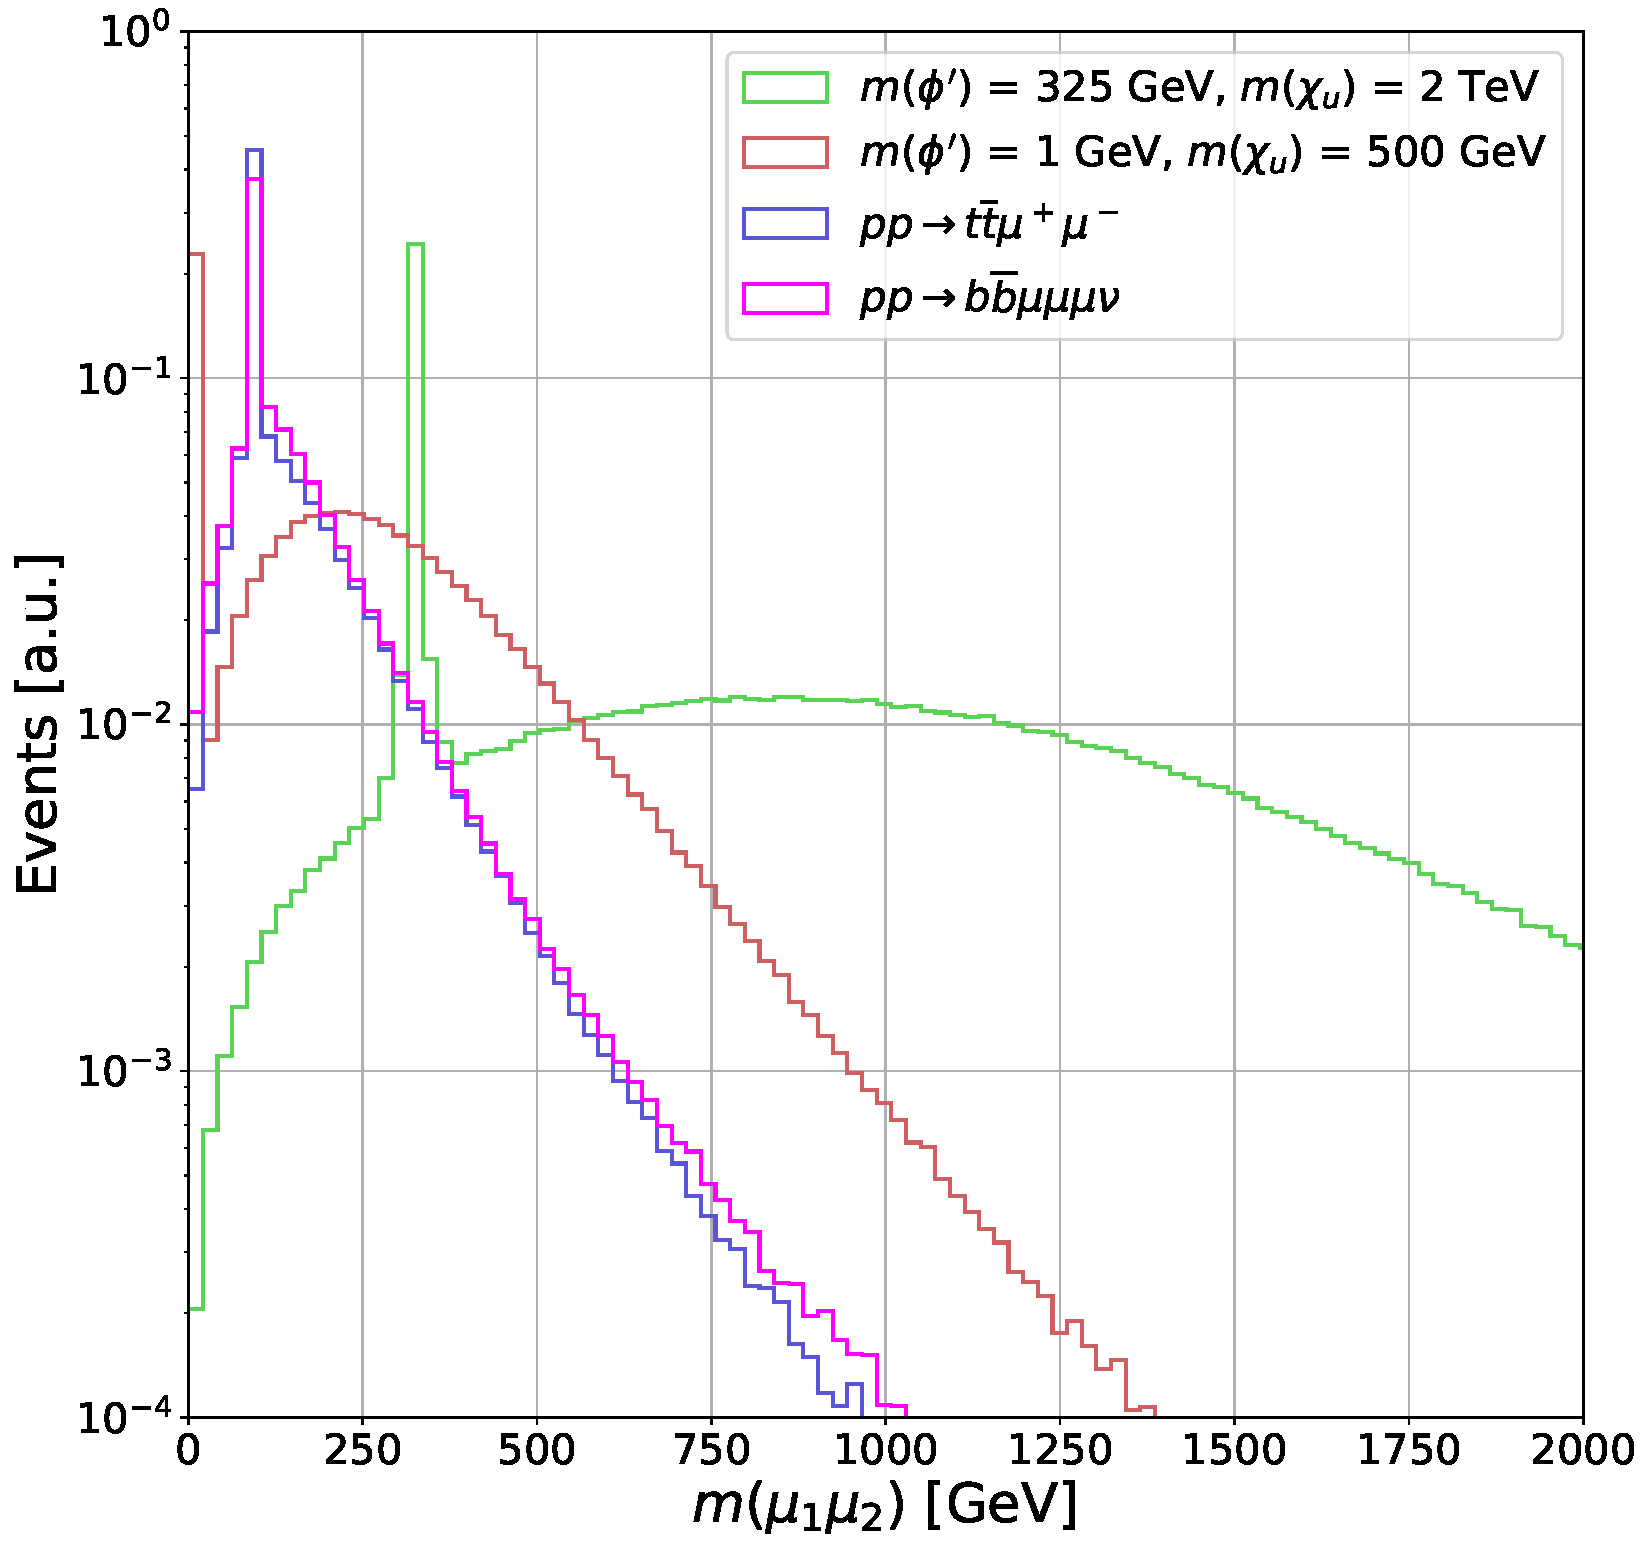
\includegraphics[width=.95\linewidth]{Images/M_mu_1_2.pdf}
\caption{Invariant mass distribution of the muon pair with the highest and second highest transverse momentum. The distributions are shown for the two main SM background processes and two signal benchmark points.\label{fig:_mu12}}
\end{figure}

We explore the performance of a diverse set of machine learning models, specifically three neural networks of differing architectures and a BDT algorithm. To ensure robust model assessment, we employed a standard 90-10 train-test split of the dataset, partitioning it into a 90\% portion for training and a 10\% portion for testing. This division allows us to gauge the generalization capabilities of our models on unseen data.  

The training and evaluation of the BDT were carried out in a high-performance computing environment. Specifically, an Nvidia A100 GPU was used. The canonical \texttt{PyTorch}~\parencite{paszke2019} deep learning framework was employed for configuring, training, and evaluating the neural networks. PyTorch is well-regarded for its flexibility and performance in deep learning applications.

For the BDT algorithm, we used hyperparameters $\eta=0.3$, $\gamma = 0$, and $\texttt{max\_depth} = 6$. The \texttt{XGBoost}~\parencite{chen_xgboost_2016} library was used for the implementation of the Boosted Decision Tree algorithm. It offers high efficiency, optimization, and interpretability, making it a suitable choice for this particular task. 

\begin{figure}
\centering
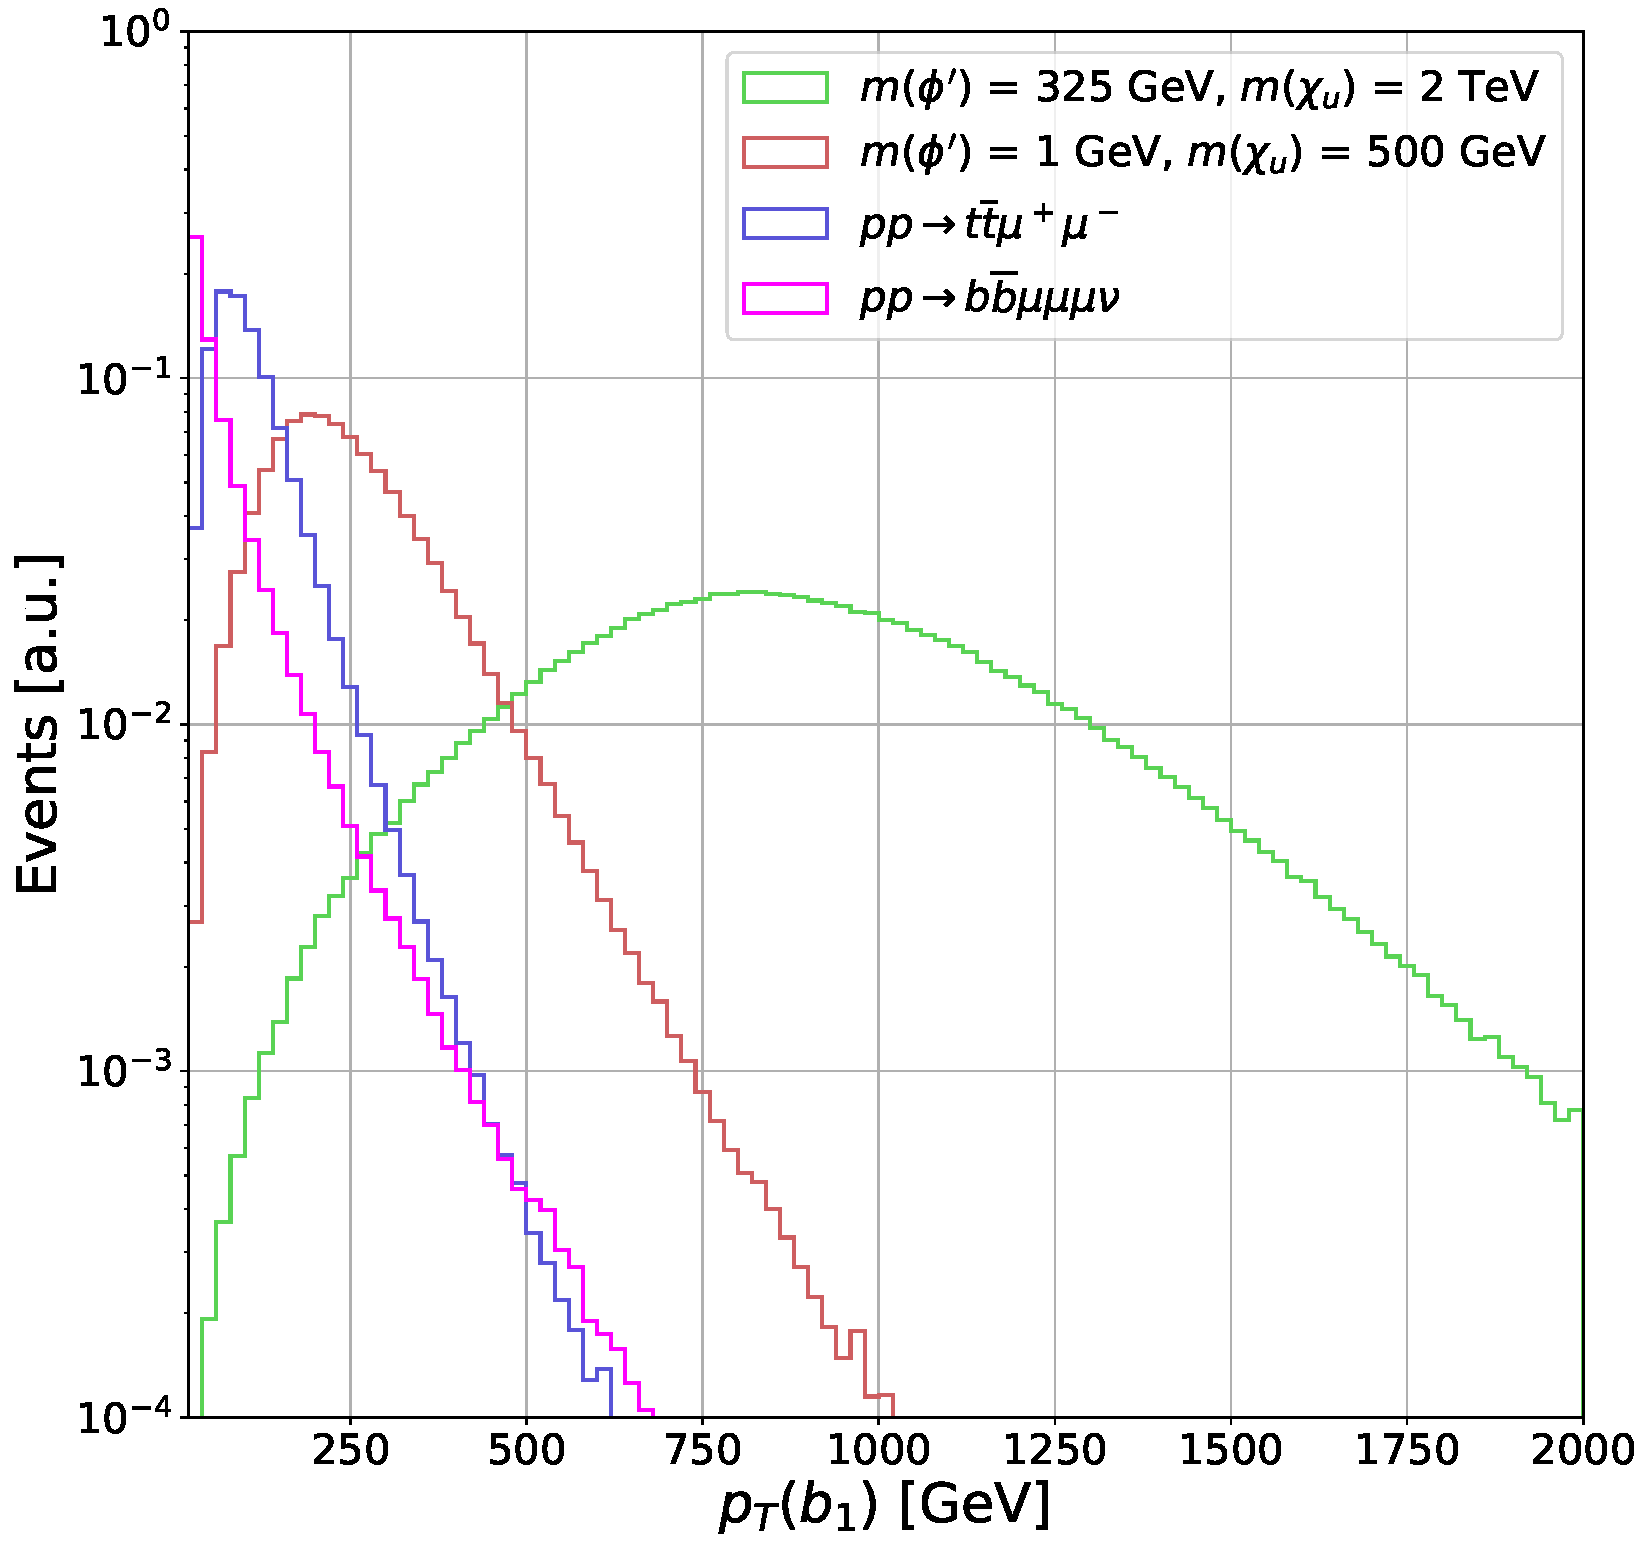
\includegraphics[width=.75\linewidth]{Images/PT_b1.pdf}
\caption{Transverse momentum distribution of the leading \textrm{b}-quark jet candidate. The distributions are shown for the two main SM background processes and two signal benchmark points.\label{fig:pTb1}}
\end{figure}

\begin{figure}
\centering
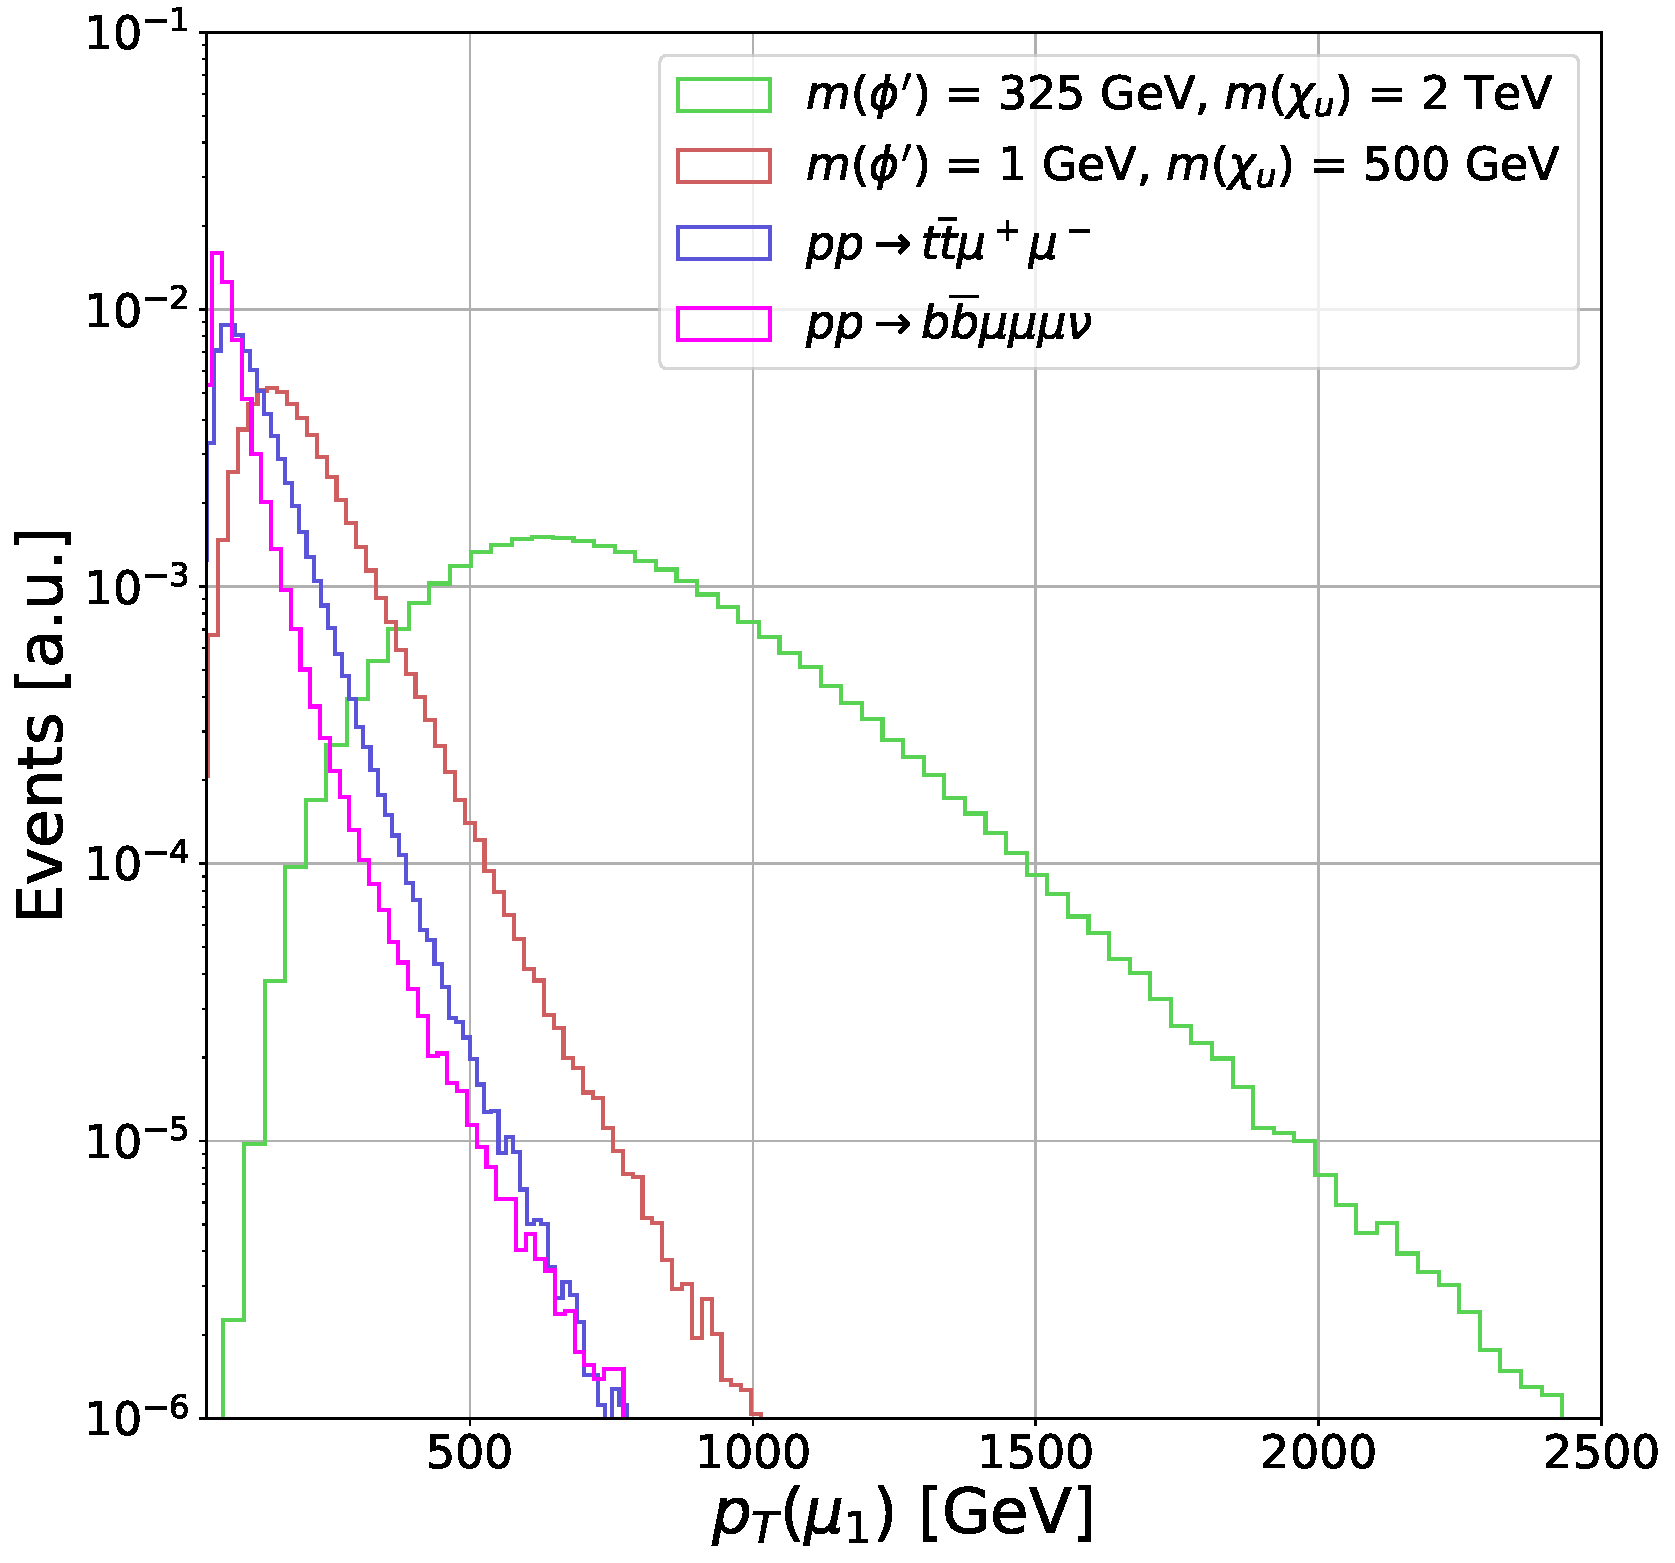
\includegraphics[width=.75\linewidth]{Images/PT_mu1_1.pdf}
\caption{Transverse momentum distribution of the leading muon candidate. The distributions are shown for the two main SM background processes and two signal benchmark points.\label{fig:pTmu1}}
\end{figure}

\begin{table}
    \centering
    \begin{tabular}{c  c  c}
    \hline
    { Model} & { Train/Test Acc. } & { Training Time} \\
    \hline
    \small
    BDT & N.A./0.9993  & 6s\\
    Neural Network 1 & 0.9999/0.9997 & 1h 58m \\
    Neural Network 2 & 0.9999/0.9998 & 2h 12m \\
    Neural Network 3 & 0.9999/0.9998 & 2h 32m\\
    \hline
    \end{tabular}
    \caption{Train/test results for the ML models.}
    \centering
\end{table}

It is worth mentioning that we experimented with deep neural networks of various architectures. Although we found that they yield similar signal sensitivity to the BDT, the complex nature of the studies in this
work (particle objects considered, experimental constraints in a high luminosity LHC, etc.) motivates the use of a BDT over a deep neural network because of its usefulness, efficiency, and simplicity in understanding the machine learning output in addition to significantly shorter training times. Therefore, we perform our proceeding analysis using the BDT. The outcomes of our model training and evaluation are presented in Table 3. 

\section{Results}\label{sec:results}
Figures~\ref{fig:_mu12},~\ref{fig:pTb1}, and~\ref{fig:pTmu1} show relevant kinematic distributions for two benchmark signal points and the dominant SM backgrounds, using the subset of events passing the pre-selections defined above. The signal benchmark points in these figures are $m(\phi^{'}) = 325 \, \mathrm{GeV}$, $m(\chi_{\mathrm{u}}) = 2\, \mathrm{TeV}$, and $m(\phi^{'}) = 1 \, \mathrm{GeV}$, $m(\chi_{\mathrm{u}}) = 500\, \mathrm{GeV}$. The distributions are normalized such that the area under the curve is unity. These distributions correspond to the reconstructed mass, $m(\mu_{1}, \mu_{2})$, between the two muon candidates with the highest transverse momentum ($\mu_{1}$ and $\mu_{2}$), 
the transverse momentum of the b-jet candidate with the highest transverse momentum $p_{\mathrm{T}}$ ($\mathrm{b_{1}}$), and the muon candidate with the highest transverse momentum $p_{\mathrm{T}}$ ($\mu_{1}$), respectively. 
These distributions are among the variables identified by the BDT algorithm with the highest signal to background discrimination power (see Figure~\ref{fig:feature_importance}).

As can be seen from Figure~\ref{fig:_mu12}, the $\phi'$ mass can be reconstructed through its associated muon decay pair, which is observed as a peak in the $m(\mu_{1}, \mu_{2})$ distribution around the expected $m(\phi')$ value, and has low- and high-mass tails which are a consequence of cases where the leading and/or subleading muon is not from the $\phi'$ decay, but rather from the associated $\mathrm{W}$ boson from the $\chi_{\mathrm{u}}$ decay. For the backgrounds, muons come from \textrm{Z} (\textrm{W}) decays. Therefore, the $m(\mu_{1}, \mu_{2})$ background distributions show a peak near $m_{\mathrm{W/Z}}$, combined with a broad distribution indicative of the combination of two muon candidates from different decay vertices. We note that the $\phi'\to\mu^{+}\mu^{-}$ decay width depends on the square of the $\phi'\to\mu^{+}\mu^{-}$ coupling and  $\frac{m_{\mu}^{2}}{m(\phi')^{2}}$ and is thus suppressed by the relatively small muon mass. For the new physics phase space considered in this paper, the $\phi'$ decay width is less than 1\% of the $\phi'$ resonant mass. Furthermore, as indicated previously, the signal/background interference effects are small and negligible compared to effects from experimental resolution. Therefore, the width of the $m(\mu_{1}, \mu_{2})$ signal distributions is driven by the experimental resolution in the reconstruction of the muon momenta, as well as the probability that the two leading muons are the correct pair from the $\phi'$ decay. Since the probability that the two highest-$p_{\mathrm{T}}$ muons are the correct pair from the $\phi'\to\mu^{+}\mu^{-}$ decay depends on $m(\phi')$ and $m(\chi_\mathrm{u})$, it is important to include all possible combinations of dimuon pairs (i.e., $m(\mu_{1}, \mu_{3})$ and $m(\mu_{2}, \mu_{3})$) in the training of the BDT. 

Figure~\ref{fig:pTb1} shows the  distribution for the \textrm{b}-jet candidate with the highest $p_{\mathrm{T}}$, $p_{\mathrm{T}}(\mathrm{b}_1)$, for the same simulated samples shown in Figure~\ref{fig:_mu12}. Based on the signal topology and our choice of parameter space (i.e., $m(\chi_\mathrm{u}) > m_{\mathrm{t}}$), it is expected that the leading $\mathrm{b}$-jet candidate comes from the $\chi_\mathrm{u}$ decay, with an average $p_{\mathrm{T}}$ close to $\frac{m(\chi_\mathrm{u}) - m_{\mathrm{W}}}{2}$, as observed in Figure~\ref{fig:pTb1}. For the $\mathrm{t} \overline{\mathrm{t}} \mu^{+}\mu^{-}$ background, the \textrm{b}-jet candidates come from top-quark decays. Therefore, their average transverse momentum is expected to be $\frac{m_{\mathrm{t}} - m_{\mathrm{W}}}{2} \approx 45$~\textrm{GeV}, as observed in Figure~\ref{fig:pTb1}. On the other hand, the \textrm{b}-jet candidates for the $\mathrm{b} \overline{\mathrm{b}}\mu\mu\mu\nu$ background can come from off-mass-shell $\mathrm{Z}^{*}/\gamma^{*}$, and thus typically have an even softer spectrum in comparison to the $\mathrm{t} \overline{\mathrm{t}} \mu^{+}\mu^{-}$ background.

Figure~\ref{fig:pTmu1} shows the  distribution for the muon candidate with the highest $p_{\mathrm{T}}$, $p_{\mathrm{T}}(\mu_{1})$. Similar to Figure~\ref{fig:pTb1}, when $m(\chi_\mathrm{u}) > m_{\mathrm{t}}$ it is expected that the leading muon candidate comes from the $\chi_\mathrm{u}$ decay, with an average $p_{\mathrm{T}}$ of approximately $\frac{m(\chi_\mathrm{u}) - m_{\mathrm{W}}}{4}$, as observed in Figure~\ref{fig:pTmu1}. For the major SM backgrounds, the muon candidates come from Z/W/$\gamma^{*}$ decays. Therefore, their average transverse momentum is expected to be much lower, $\frac{m_{\mathrm{Z/W}}}{4} \approx 40-45$~\textrm{GeV}. This kinematic feature provides a nice handle to discriminate high $m(\chi_\mathrm{u})$ signal events amongst the large SM backgrounds, which have lower average $p_{\textrm{T}}(\mu)$ constrained by the SM weak boson masses.

In addition to these aforementioned variables in Figures~\ref{fig:_mu12}-\ref{fig:pTmu1}, several other kinematic variables were included as inputs to the BDT algorithm. In particular, 27 such variables were used in total, and these included the momenta of $\mathrm{b}$ and muon candidates; invariant masses of pairs of muons; angular differences between $\mathrm{b}$ jets and between the muons. 

As mentioned above, the variables $m(\mu_{i}, \mu_{j})$ for $i, j \neq 1$ provide some additional discrimination between signal and background when the leading muons are not a $\phi'$ decay candidate. The angular separation variables, such as $\Delta R(\mu_{i}, \mu_{j})$, are designed to be sensitive to lower mass $\phi'$, since the low rest mass of those particles means they acquire more boost, and thus smaller angular separation $\Delta R$ between the muon candidates. The trained BDT returns the discriminating power of each of its inputs, and the feature importance for each variable is shown in Figure~\ref{fig:feature_importance} for a signal benchmark point with $m(\phi')=325\, \mathrm{GeV}$ and $m(\chi_\mathrm{u})=2000\, \mathrm{GeV}$.

\begin{figure}
\centering
  \centering  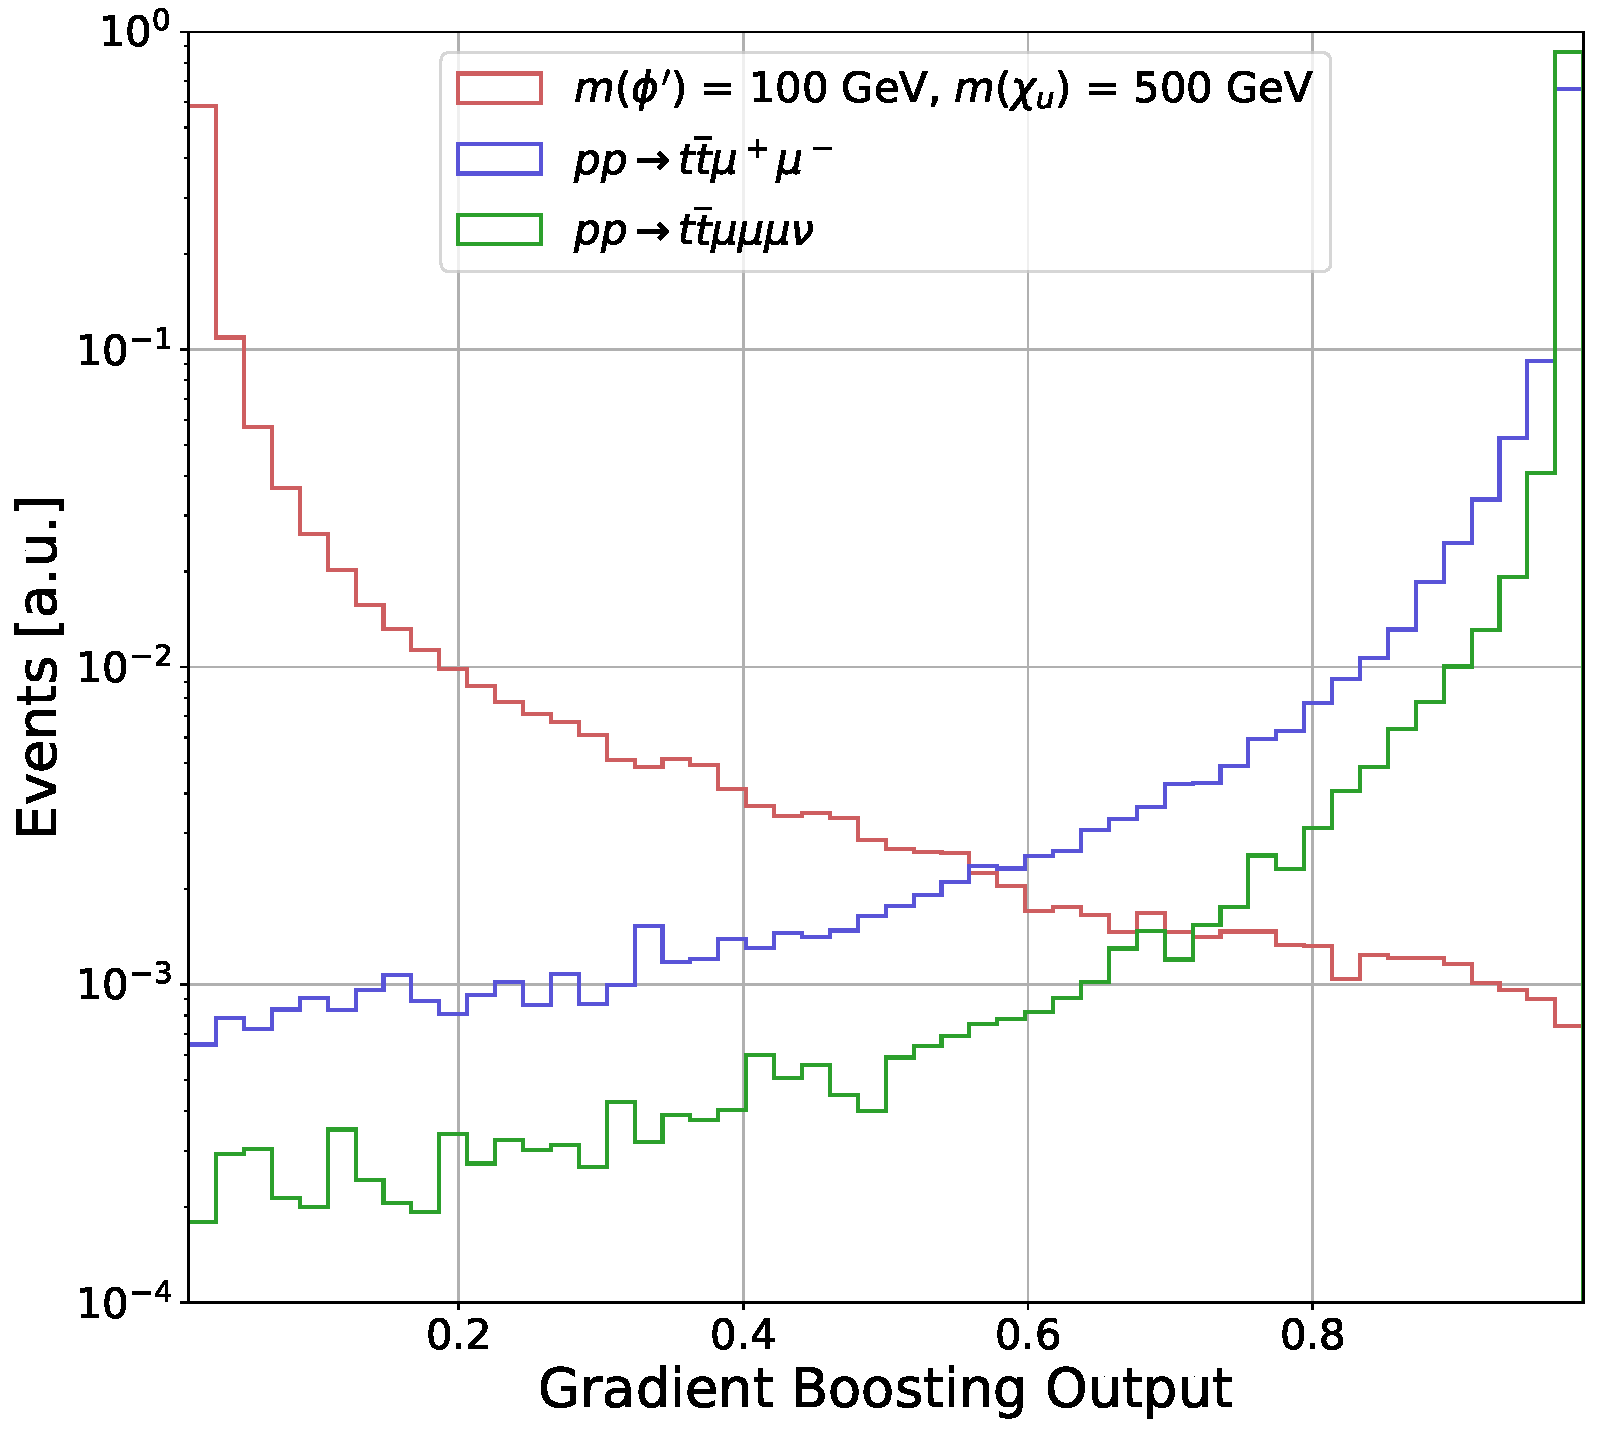
\includegraphics[width=.75\linewidth]{Images/XGB_output.pdf}
  \caption{Output of the gradient boosting algorithm for a benchmark $m(\phi') = 100$~\textrm{GeV} and $m(\chi_\mathrm{u}) = 500\, \mathrm{GeV}$ signal, and dominant backgrounds. The distributions are normalized to unity.}
  \label{fig:xgboostout}
\end{figure}

Figure~\ref{fig:xgboostout} shows  the distributions for the output of the BDT algorithm, normalized to unity, for the representative signal benchmark point of $m(\phi') = 1\, \mathrm{GeV}$, $m(\chi_\mathrm{u}) = 0.5\, \mathrm{TeV}$ and the two dominant backgrounds. The output of the BDT algorithm is a value between 0 and 1, which quantifies the likelihood that an event is either background-like (BDT output near 1) or signal-like (BDT output near 0). Figure~\ref{fig:ROC} illustrates the true positive rate (TPR), defined as the probability of correctly selecting signal events using the BDT output, plotted against the false positive rate (FPR), defined as the probability of incorrectly selecting background events. For example, for $m(\phi') = 100\, \mathrm{GeV}$ and $m(\chi_\mathrm{u}) = 500\, \mathrm{GeV}$, when signal events are selected at 65\% probability, the background is selected at about $10^{-3}$ probability. We note that the primary discriminating feature between the signal and background is the boosted b-jet $p_T$ coming from the $\chi_u$ vector-like quark. The $p_T$ of said b jet increases with $m(\chi_\mathrm{u})$, peaking at around $[m(\chi_\mathrm{u}) - m(\textrm{W})] / 2$. This enhanced boost increases the separation between signal and background, improving the performance of the BDT algorithm as $m(\chi_\mathrm{u})$ increases. 

\begin{figure}
\centering
  \centering
  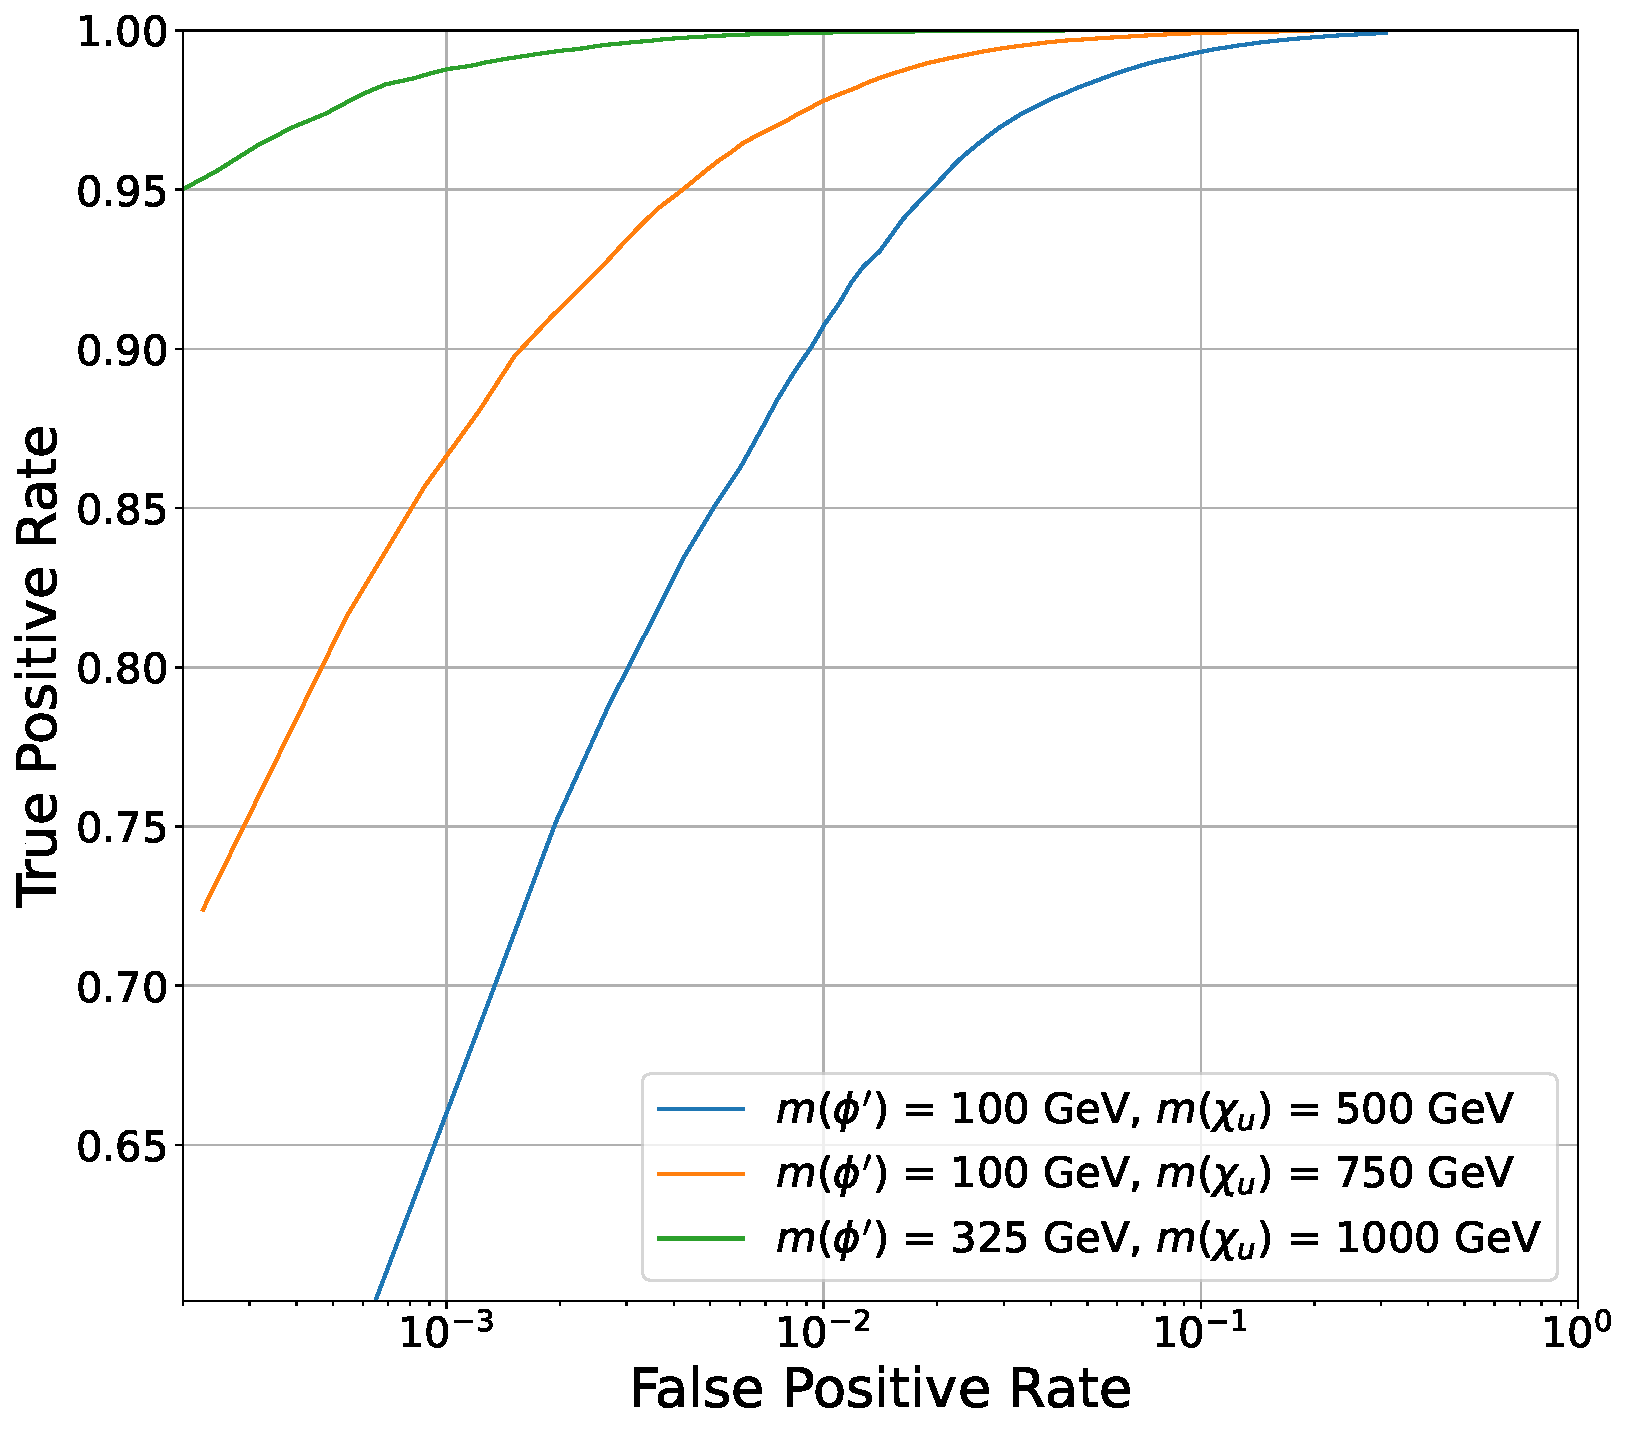
\includegraphics[width=.75\linewidth]{Images/ROC_Curve.pdf}
  \caption{Receiver operating characteristic curve of the BDT algorithm for three different signal benchmark scenarios.}
  \label{fig:ROC}
\end{figure}

\begin{figure}
\centering
  \centering
  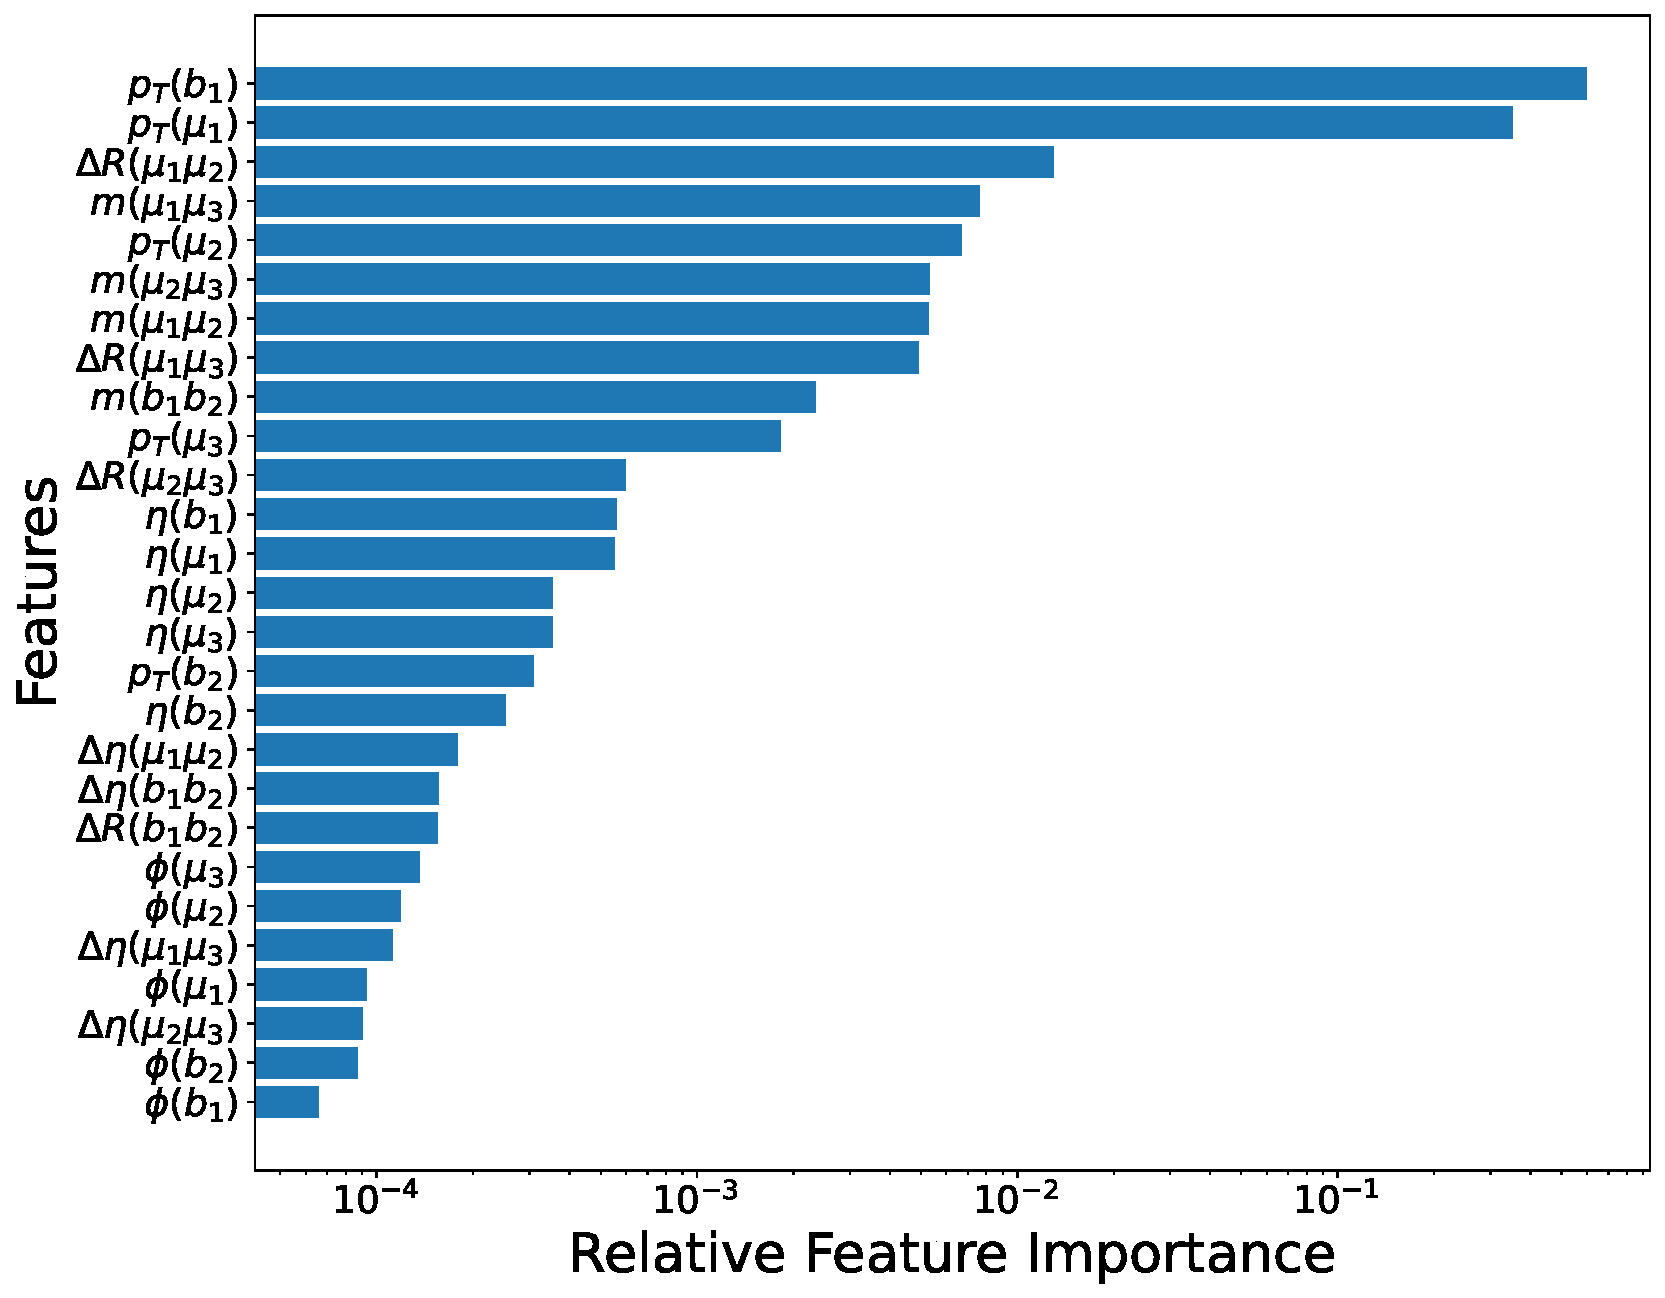
\includegraphics[width=.75\linewidth]{Images/feature_importance.pdf}
  \caption{Relative importance of features in training for a benchmark signal scenario with $m(\phi')=325\, \mathrm{GeV}$ and $m(\chi_\mathrm{u})=2000\, \mathrm{GeV}$.}
  \label{fig:feature_importance}
\end{figure}

The outputs from the BDT machine learning algorithm are used to perform a profile-bin likelihood analysis to estimate the signal significance for a luminosity of 3000 $\mathrm{fb^{-1}}$, corresponding to the expected amount of collected data by the end of the LHC era. For this purpose, the BDT distributions are normalized to cross section times pre-selection efficiency times luminosity for the different signal models. The significance is then calculated using the expected bin-by-bin yields of the BDT output distribution in a profile likelihood fit, using the ROOTFit~\parencite{Butterworth:2015oua} package developed by CERN. The expected signal significance $Z_\text{sig}$ is calculated using the probability of obtaining the same test statistic for the  signal plus background and the signal-null hypotheses, defined as the local $p$-value. Similar to Refs.~\parencite{Florez:2021zoo, Florez:2019tqr, Florez:2018ojp, Florez:2017xhf, VBFZprimePaper, Florez:2016lwi, Leonardi_2020}, the significance  corresponds to the point where the integral of a Gaussian distribution between $Z_\text{sig}$ and $\infty$ results in a value equal to the local $p$-value. The estimation of $Z_\text{sig}$ incorporates  systematic uncertainties. The uncertainty values have been included as nuisance parameters, considering lognormal priors for normalization and Gaussian priors for uncertainties associated with the modeling of the shapes similar to Refs.~\parencite{natalia2021longtermlhcdiscoveryreach, PhysRevD.103.095001}. 

The systematic uncertainties that have been included result from experimental and theoretical constraints.   A 1-5\% systematic uncertainty, depending on the simulated MC sample, has been included to account for the choice of Parton Distribution Function (PDF) set. The systematic uncertainty effect was incorporated following the PDF4LHC~\parencite{Butterworth:2015oua} recommendations. This systematic uncertainty has a small impact on the expected event yields for signal and background, but it does not affect the shape of the BDT output distribution. We additionally considered theoretical uncertainties related to the absence of higher-order contributions to the signal cross sections, which can change the pre-selection efficiencies and the shapes of kinematic variables used as inputs to the BDT algorithm. This uncertainty was calculated by varying the renormalization and factorization scales by $\times 2$, and studying the resulting change in the bin-by-bin yields of the BDT distributions. They are found to be at most 2\% in a given bin. 
%Additional theoretical uncertainties were taken into account, including the potential impact of higher-order contributions to the signal cross sections. These contributions can influence the pre-selection efficiency and shapes of kinematic distributions utilized by the BDT algorithm. The uncertainty associated with this is determined by adjusting the renormalization and factorization scales by a factor of two relative to the nominal value and considering the complete change in the bin-by-bin yields of the BDT output distribution. The maximum impact of these uncertainties in a given bin is found to be 1-3\%. 

Regarding experimental uncertainties, following experimental measurements from CMS on the estimation of the integrated luminosity, a conservative 3\% effect has been included~\parencite{lumiRef}. A 5\% systematic uncertainty associated with the reconstruction and identification of $\mathrm{b}$-quark jets has been included, independent of $p_\mathrm{T}$ and $\eta$ of the $\mathrm{b}$-jet candidates. According to Ref.~\parencite{CMSbtag}, this uncertainty is correlated between signal and background processes with genuine  \textrm{b}-jets and is also correlated across BDT bins for each process. For muons, we include a 2\% uncertainty associated with the reconstruction, identification, and isolation requirements, and a 3\% systematic uncertainty to account for scale and resolution effects on the momentum and energy measurement. 
%For muon reconstruction, identification, and isolation requirements, there is a 1-2\% uncertainty, while a 1-3\% systematic uncertainty is applied to variations in energy/momentum scale and resolution. 
We consider jet energy scale uncertainties ranging from 2-5\%, contingent on $\eta$ and $p_\mathrm{T}$, resulting in shape-based uncertainties on the BDT output distribution. Jet energy scale uncertainties were assumed to range from 1-5\%, contingent on $\eta$ and $p_\mathrm{T}$. These assumptions lead to shape-based uncertainties on the BDT output distribution, varying from 1-2\%. Additionally, we include  a 10\% systematic uncertainty to account for errors in the signal and background predictions. Considering all the various sources of systematic uncertainties, our conservative  estimate yields a total effect of about 20\%. 

Figure~\ref{fig:/significance_3000} shows the expected signal significance considering an integrated luminosity of 3000 $\mathrm{fb^{-1}}$. The significance is shown as a heat map in a two-dimensional plane for different $\phi'$ and $\chi_{\mathrm{u}}$ masses. The x-axis corresponds to $m(\chi_\mathrm{u})$, the y-axis to $m(\phi')$, and the heat map to log$_{10}(\mathrm{Z}_{sig})$. The white dashed lines are contours of constant signal significances of $1.69 \sigma$,  $3\sigma$ and  $5\sigma$ to represent regions of possible exclusion, evidence of new physics, and discovery, respectively. Under these conditions, $\phi'$ ($\chi_{\mathrm{u}}$) masses ranging from 1 to 325 \textrm{GeV} (500 to 1800 \textrm{GeV}) can be probed. The range for a discovery with $5\sigma$ signal significance varies from $\chi_{\mathrm{u}}$ masses from $m(\chi_{\mathrm{u}}) = 770$-1100 \textrm{GeV}, depending  $m(\phi^{'})$. For large $m(\chi_\mathrm{u})$, the significance is almost independent of $m(\phi')$ because the primary discriminating feature—the boosted $b$-quark originating from $\phi'$—is driven predominantly by the large $m(\chi_\mathrm{u})$, with the kinematic impact of $m(\phi')$ being relatively negligible.


\begin{figure}[]
\centering
  \centering
  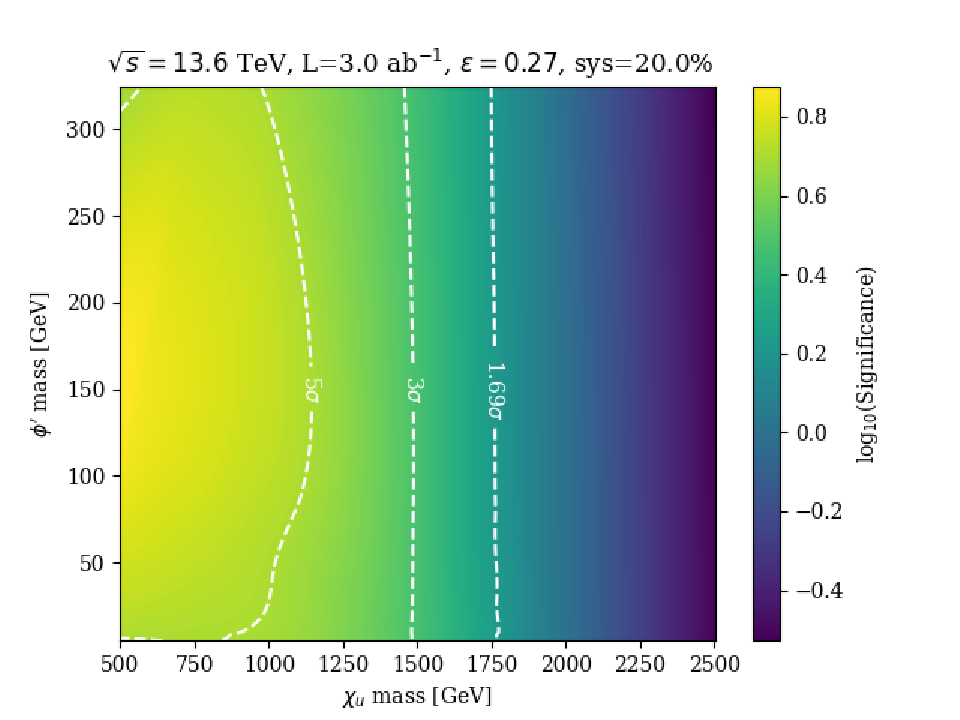
\includegraphics[width=.85\linewidth]{Images/significance.pdf}
  \caption{Signal significance for the high luminosity LHC era, considering with 3000  $\mathrm{fb}^{-1}$ of collected data.}
  \label{fig:/significance_3000}
\end{figure}

\section{Discussion}\label{sec:discussion}

The LHC will continue to run with pp collisions at $\sqrt{s} = 13.6$~\textrm{TeV} for the next decade. Given the increase in the integrated luminosity expected from the high-luminosity program, it is important to consider unexplored new physics phase space that diverges from the conventional assumptions made in many BSM theories, and which could have remained hidden in processes that have not yet been thoroughly examined. It is additionally crucial to explore advanced analysis techniques, in particular the use of artificial intelligence algorithms, to enhance the probability of detecting these rare corners where production cross sections are lower and discrimination from SM backgrounds is difficult. 

In this work, we examine a model based on a $U(1)_{T^3_R}$ extension of the SM, which can address various conceptual and experimental issues with the SM, including the mass hierarchy between generations of fermions, the thermal dark matter abundance, and the muon $g - 2$, $R_{(D)}$, and $R_{(D^*)}$ anomalies. This model contains a light scalar boson $\phi'$, with potential masses below the electroweak scale, and~\textrm{TeV}-scale vector-like quarks $\chi_\mathrm{u}$. We consider the scenario where the scalar $\phi'$ has family non-universal fermion couplings and $m(\phi') \ge 1$~\textrm{GeV}, as was suggested in Ref.~\parencite{Dutta2020}, and thus the $\phi^{\prime}$ can primarily decay to a pair of muons. Previous works in Refs.~\parencite{Dutta2023, Banerjee_2016} considered scenarios motivating a search methodology with a merged diphoton system from $\phi' \to \gamma\gamma$ decays. The authors of Ref~\parencite{Dutta2023}, in which $m(\phi') < 1$~\textrm{GeV},  indeed pointed out that if the $\phi'$ is heavier than about 1~\textrm{GeV}, then decays to $\mu^+ \mu^-$ can become the preferable mode for discovery, which is the basis for the work presented in this paper. We further note that the final state topology studied in this paper would represent the most important mode for discovery at $m(\phi') < 2 m_{\mathrm{t}}$ where the $\phi' \to \mathrm{t\bar{t}}$ decay is kinematically forbidden. 

The main result of this paper is that we have shown that the LHC can probe the visible decays of new bosons with masses below the electroweak scale, down to the~\textrm{GeV}-scale, by considering the simultaneous production of heavy QCD-coupled particles, which then decay to the SM particles that contain large momentum values and can be observed in the central regions of the CMS and ATLAS detectors. The boosted system combined with innovative machine learning algorithms allows for the signal extraction above the lower-energy SM background. The LHC search strategy described here can be used to discover the prompt decay of new light particles.  An important conclusion from this paper is that the detection prospects for low-mass particles are enhanced when it is kinematically possible to simultaneously access the heavy degrees of freedom which arise in the UV completion of the low-energy model.  This specific scenario in which the couplings of the light scalars are generationally dependent, with important coupling values to the top quark, is an ideal example which would be difficult to directly probe at low energy beam experiments.

The proposed data analysis represents a competitive alternative 
to complement searches already being conducted at the LHC, allowing us to probe $\phi'$ masses from 1 to 325 \textrm{GeV}, for $m(\chi_{\mathrm{u}})$ values up to almost 2~\textrm{TeV}, at the HL-LHC. Therefore, we strongly encourage the ATLAS and CMS Collaborations to consider the proposed analysis strategy in future new physics searches. 
\chapter{Discussion and results}

\appendix
\renewcommand{\theequation}{{\Alph{chapter}.\arabic{equation}}}
\renewcommand{\thefigure}{{\Alph{chapter}.\arabic{figure}}}
\renewcommand{\thetable}{{\Alph{chapter}.\arabic{table}}}
\chapter{Publications}
\lipsum
\newpage
\phantomsection
\addcontentsline{toc}{section}{On the sensitivity reach of vectorial leptoquark production with preferential couplings to third generation fermions at the LHC}
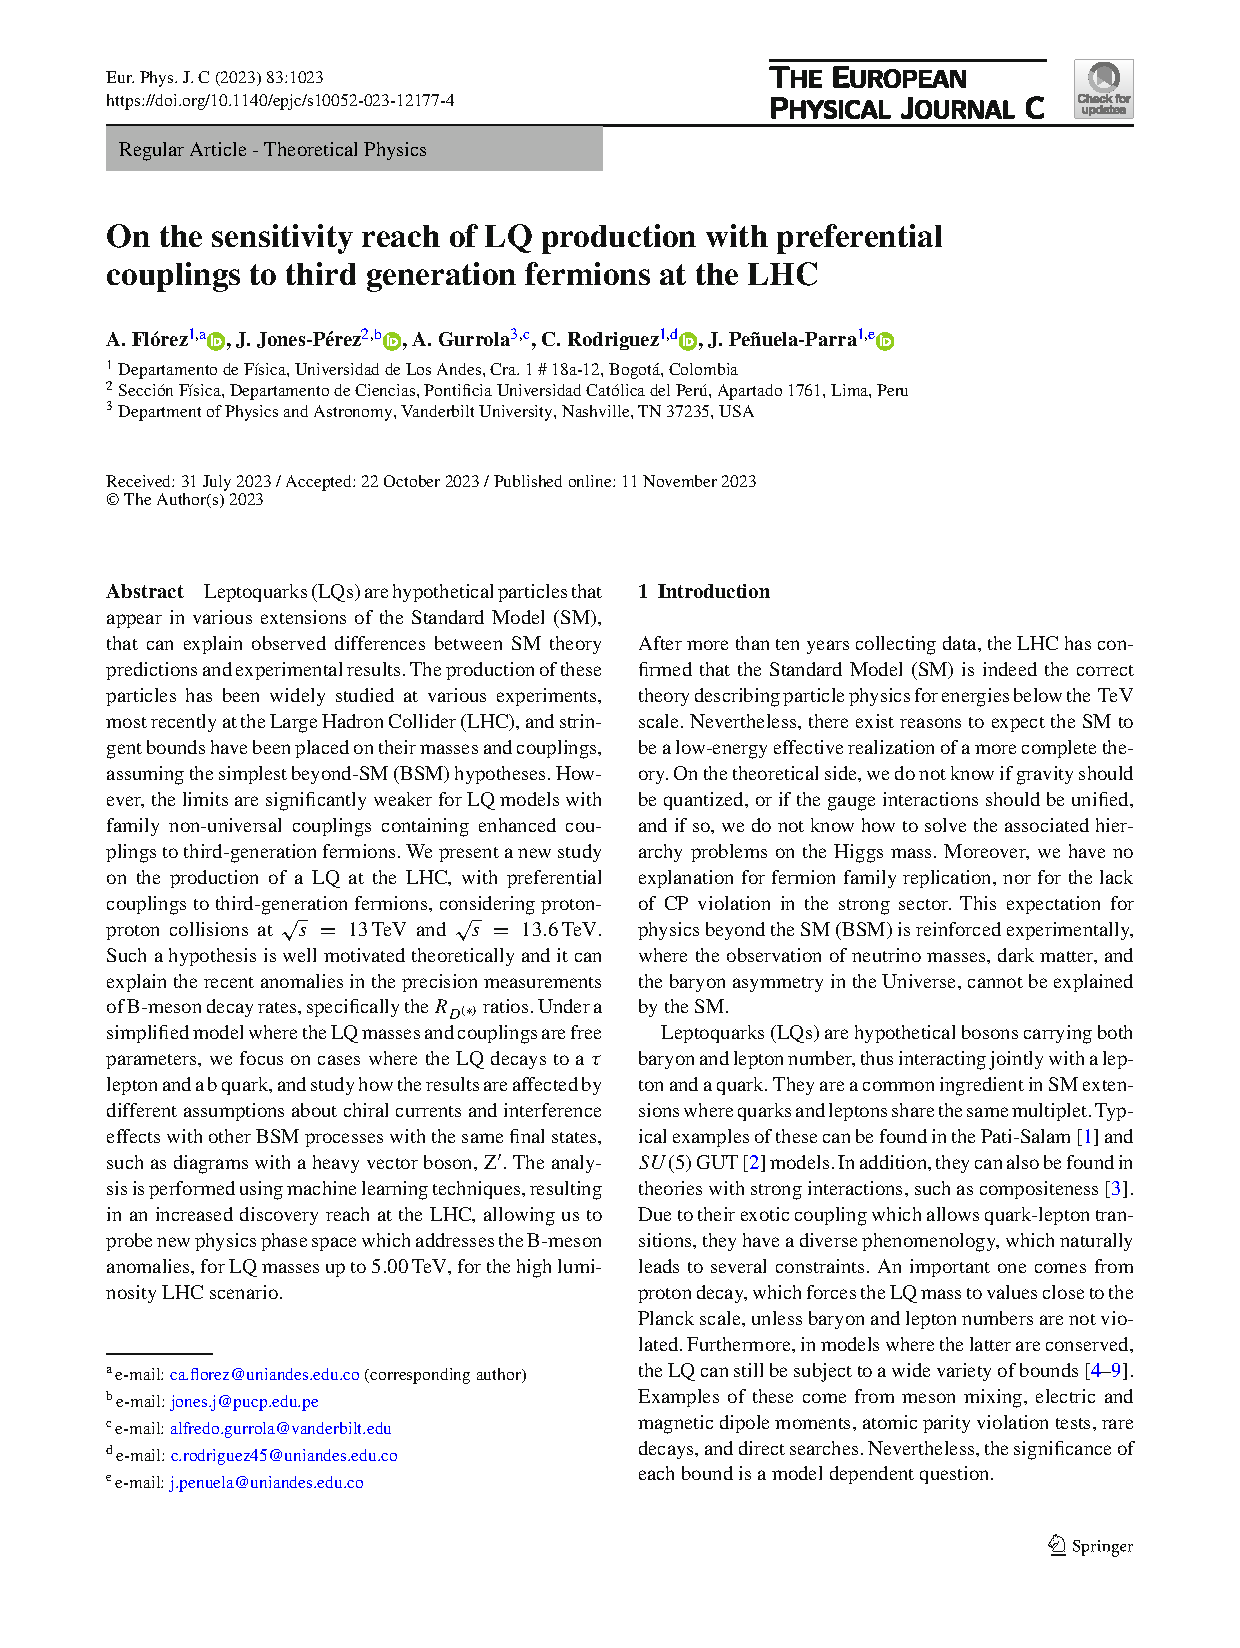
\includepdf[pages=-,offset= 16 0]{papers/s10052-023-12177-4.pdf}
$ $
\newpage
\phantomsection
\addcontentsline{toc}{section}{Probing light scalars and vector-like quarks at the high-luminosity LHC}
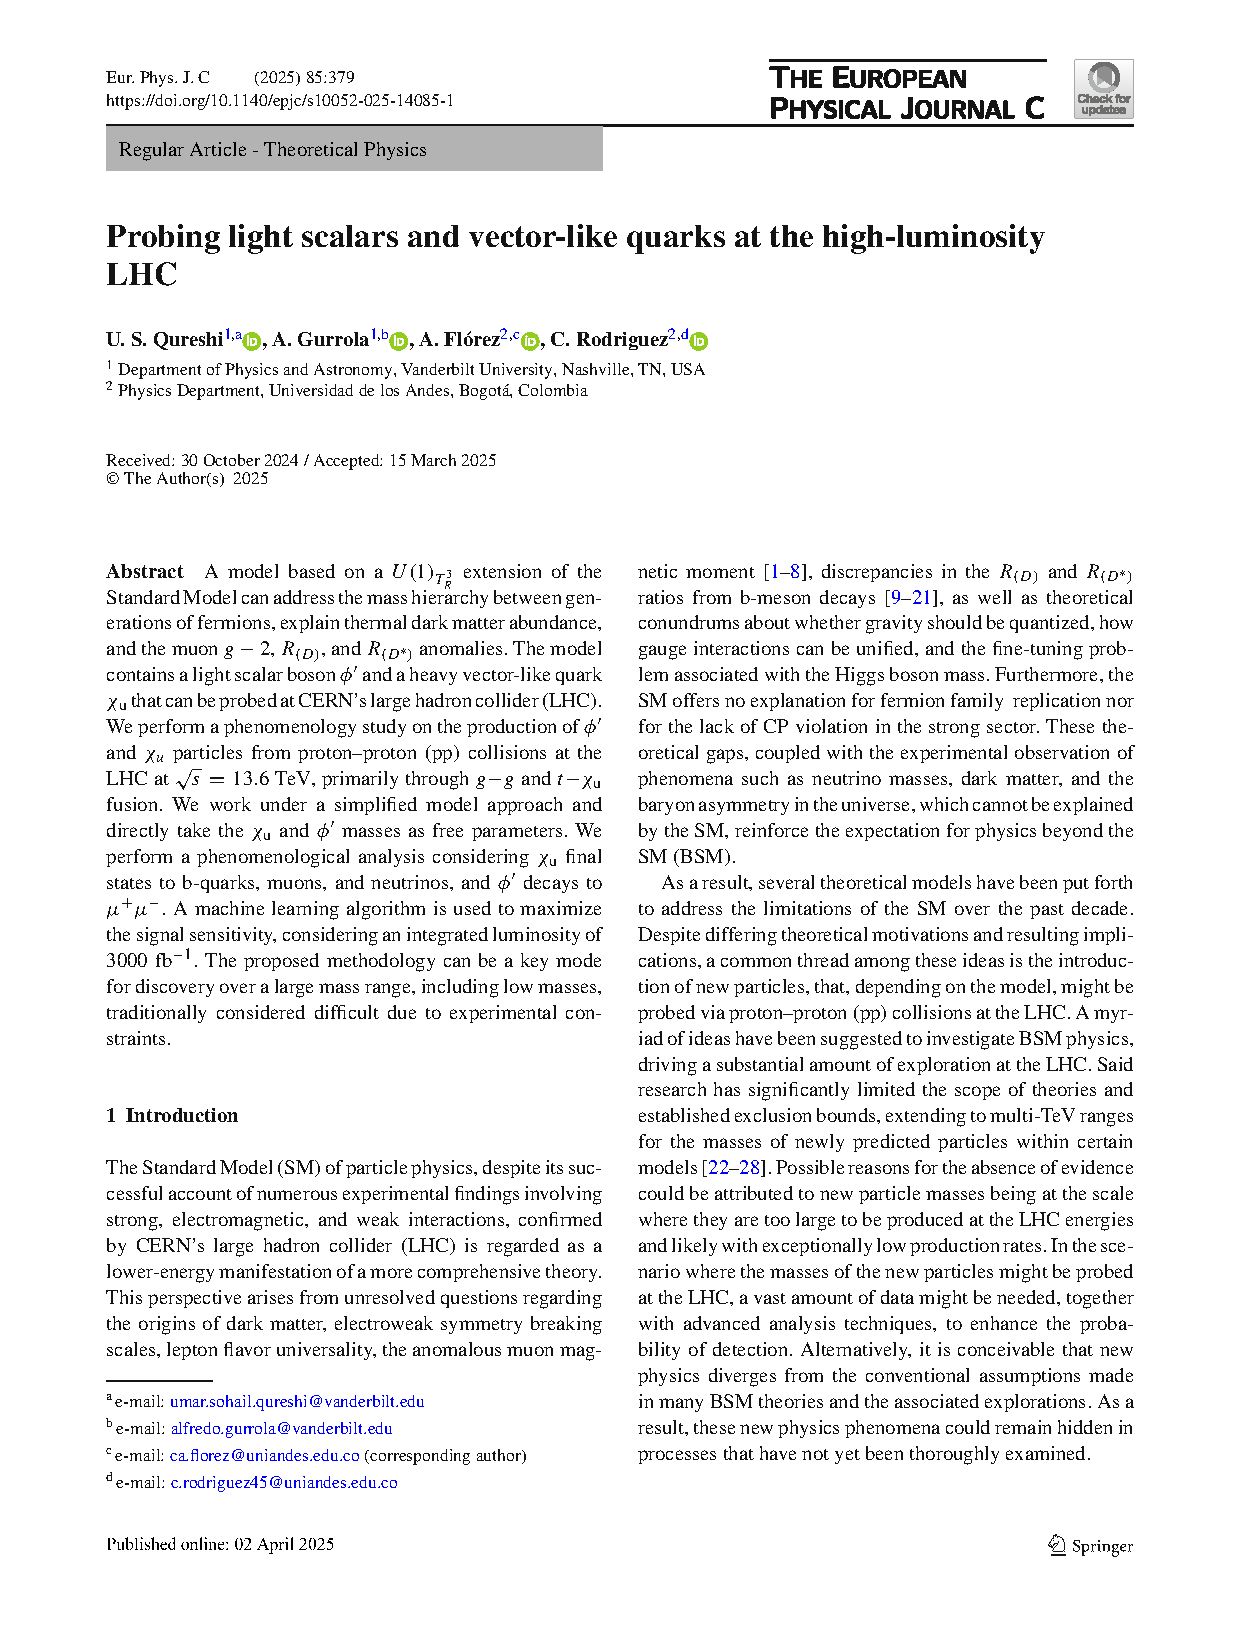
\includepdf[pages=-,offset= 16 0]{papers/s10052-025-14085-1.pdf}
\chapter{The CMS Detector and Physical Observables}
\lipsum
\chapter{Standard Model Simulation}
\lipsum

\chapter{Principle of maximum likelihood and hypothesis testing}
\lipsum
\chapter{Supervised Learning}
\lipsum

\section{The Classification Problem}
\lipsum

\section{The Regression Problem}
\lipsum
\chapter{Framework}
\chapter{Madgraph Scripts}

\section{Background Scripts}

\begin{tcolorbox}[title=Background MadGraph Script]
    \lstinputlisting{scripts/bkg_outputs.mg5}
\end{tcolorbox}
\lipsum

\end{document}
